% !TeX program = xelatex
% Compile với XeLaTeX (Overleaf: Menu > Compiler > XeLaTeX)
% BẢN RÚT GỌN 45 PHÚT (41 slide) — copy & tinh chỉnh từ bộ slide gốc 190 slide trong ../ (KHÔNG xoá bản gốc)
\documentclass[aspectratio=169,9pt]{beamer}

\usepackage{fontspec}
\setmainfont{Noto Serif}
\setsansfont{Noto Sans}
\usepackage{polyglossia}
\setmainlanguage{vietnamese}

\usepackage{amsmath,amssymb}
\usepackage{graphicx}
\usepackage{booktabs}
\usepackage{tikz}
\usetikzlibrary{arrows.meta,positioning,shapes,fit}
\usepackage{caption}
\captionsetup{font=scriptsize,labelfont=bf}
\usepackage{etoolbox}
\AtBeginEnvironment{itemize}{\setlength{\itemsep}{1pt}\setlength{\parskip}{0pt}\setlength{\topsep}{1pt}}
\AtBeginEnvironment{enumerate}{\setlength{\itemsep}{1pt}\setlength{\parskip}{0pt}\setlength{\topsep}{1pt}}
\setlength{\abovedisplayskip}{4pt}
\setlength{\belowdisplayskip}{4pt}
\setlength{\abovedisplayshortskip}{2pt}
\setlength{\belowdisplayshortskip}{2pt}

\usetheme{Madrid}
\usecolortheme{seahorse}
\setbeamertemplate{navigation symbols}{}
\setbeamertemplate{footline}[frame number]
\setbeamerfont{footnote}{size=\tiny}
\setbeamerfont{section in toc}{size=\tiny}
\setbeamerfont{subsection in toc}{size=\tiny}

\title[SADGS: 3DGS \& Tăng tốc (45 phút)]{Quy trình Render 3D Gaussian Splatting\\và Cải tiến SADGS (SADGS)}
\subtitle{Bản rút gọn 45 phút — Từ nền tảng đến Adaptive Density Control}
\author{Digital Twin GS}
\date{\today}

% Thư mục ảnh vẫn trỏ về figures/ gốc (Slides67/figures), vì file này nằm trong Slides67/Slides45min/
\graphicspath{{../figures/}{../../BOOK/fastergs_merge_figures/}{../../BOOK/adc_figures/}}

\begin{document}

% Lưu ý: KHÔNG đặt \titlepage ở đây — Slide 1 (trang bìa) đã nằm sẵn
% trong part45_01.tex để tránh trùng lặp trang bìa.

% ===================== 41 SLIDE RÚT GỌN, CHIA 10 FILE CHO 10 BOT =====================
% part45_01.tex : Slide 1-4   (Bìa/agenda, Động lực, 3D Gaussian là gì)
% part45_02.tex : Slide 5-8   (Hiệp phương sai, Màu SH, Pipeline render, EWA splatting)
% part45_03.tex : Slide 9-12  (Compact Box, Alpha blending, Tổng kết render, Loss)
% part45_04.tex : Slide 13-16 (Gradient biên, Tổng kết training loop, ADC tổng quan, Tích luỹ gradient)
% part45_05.tex : Slide 17-20 (Gradient cancellation, Clone, Split, Prune multi-view)
% part45_06.tex : Reset opacity, Sơ đồ quyết định densify
% part45_07.tex : Slide 25-28 (Top-k vs Multinomial, Toy model, So sánh ADC, Kết quả 3 kịch bản)
% part45_08.tex : Slide 29-32 (Tổng kết 5 cải tiến, Vì sao 3DGS chậm, 3 đòn bẩy, Thác nước)
% part45_09.tex : Slide 33-38 (Cơ chế lõi structure-aware/eta [MỚI], Tổng kết 3DGS→SADGS,
%                  Colab T4, Bảng 1, Bảng 3, Giới hạn phép đo)
% part45_11.tex : Slide C (Bảng so sánh 3DGS gốc/SADGS)
%                  -- chèn giữa part45_09 và part45_10 theo thứ tự \input bên dưới
% part45_10.tex : Slide 39-42 (RAM vs VRAM, Tổng kết pipeline, Tổng kết cải tiến, Cảm ơn/Q&A)

% ===================== CẤU TRÚC 5 PHẦN (\section không sinh thêm trang) =====================
% Số trang giữ nguyên; \section chỉ tạo mốc điều hướng / bookmark trong PDF.

\section{Nền tảng \& Render}
% ===== FILE 1/9: Bìa, Động lực, 3D Gaussian, Hiệp phương sai, Scale khởi tạo, Scene extent, Màu SH, Lịch tăng bậc SH =====

% --- Slide: Bìa ---
\begin{frame}
\titlepage
\end{frame}

% --- Slide: Động lực ---
\begin{frame}{Vì sao 3D Gaussian Splatting?}
\footnotesize
\begin{itemize}
    \item \textbf{Bài toán đặt ra:} cho một tập ảnh chụp một cảnh từ nhiều góc, cùng camera pose ước lượng sẵn bởi
    SfM/COLMAP, hãy dựng lại một biểu diễn 3D sao cho có thể \textbf{render lại ảnh từ bất kỳ góc nhìn mới nào}
    (novel view synthesis) một cách chân thực.
    \item \textbf{NeRF (2020)} giải bài này bằng một mạng MLP ẩn ánh xạ (vị trí, hướng nhìn) $\to$ (màu, mật độ), rồi
    \textbf{ray-marching}: bắn hàng trăm điểm mẫu dọc mỗi tia sáng, gọi mạng hàng trăm lần cho mỗi pixel. Chất lượng
    cao nhưng cực chậm --- train mất hàng giờ/ngày, render cũng mất giây/khung hình vì phải lặp lại forward pass qua mạng cho từng điểm mẫu.
    \item \textbf{3D Gaussian Splatting} (Kerbl, Kopanas, Leimkühler, Drettakis --- SIGGRAPH 2023) đổi hẳn cách biểu diễn:
    thay mạng ẩn bằng \textbf{hàng trăm nghìn tới hàng triệu "Gaussian 3D" tường minh}, mỗi Gaussian là một đối tượng
    có tham số cụ thể $\{\mu,\Sigma,\alpha,c\}$ (Slide sau). Render không cần mạng nơ-ron, không cần ray-marching --- chỉ
    cần \textbf{chiếu (project) và tô (rasterize)} trực tiếp các Gaussian lên màn hình, giống hệt cách GPU vẽ tam giác
    trong đồ hoạ game truyền thống. Kết quả: train nhanh hơn nhiều lần, và quan trọng nhất --- render \textbf{thời gian thực}
    (hàng chục--hàng trăm khung hình/giây) sau khi train xong.
    \item \textbf{Nhưng còn một vấn đề chưa giải quyết trọn vẹn:} số lượng Gaussian $N$ cần bao nhiêu, đặt ở đâu, kích
    thước ra sao --- không biết trước, phải \textbf{tự động điều chỉnh trong lúc train} (đây gọi là \emph{Adaptive Density
    Control}, viết tắt ADC). Cơ chế ADC gốc chỉ dựa vào \textbf{gradient} để quyết định thêm/bớt Gaussian --- và đây
    chính là chỗ \textbf{SADGS} (Structure-Aware Densification for Gaussian Splatting) can thiệp: bổ sung thêm một tín
    hiệu đo trực tiếp \textbf{cấu trúc tần số cục bộ} của ảnh, để quyết định "đúng chỗ, đúng lúc, đúng trục" hơn.
\end{itemize}
\vspace{2pt}
\footnotesize\textbf{Lộ trình bài giảng:} (1) Biểu diễn Gaussian \& pipeline render $\to$ (2) Loss, gradient, ADC nguyên
bản của 3DGS $\to$ (3) SADGS: xây dựng tín hiệu tần số $\eta$ từ đầu, cơ chế densify/prune mới $\to$ (4) Nhìn lại một
cách trung thực: cái gì đang thật sự chạy, so sánh với bản gốc.
\end{frame}

% --- Slide: 3D Gaussian là gì ---
\begin{frame}{3D Gaussian: đơn vị biểu diễn cơ bản}
\scriptsize
Toàn bộ cảnh được biểu diễn bằng một \textbf{tập hợp các Gaussian 3D} --- mỗi Gaussian là một hàm mật độ liên tục
trong không gian, tâm tại $\mu\in\mathbb{R}^3$, "độ loang" theo ma trận hiệp phương sai $\Sigma\in\mathbb{R}^{3\times3}$:
\[
\boxed{\;G(x)=\exp\!\Big(-\tfrac12(x-\mu)^\top\Sigma^{-1}(x-\mu)\Big)\;}
\]
Có thể hình dung mỗi Gaussian như một \textbf{"cục mây mờ" hình ellipsoid}: đậm đặc nhất ở tâm $\mu$, mờ dần ra biên
theo hình dạng do $\Sigma$ quyết định. Mỗi Gaussian mang theo $4$ nhóm tham số \textbf{học được bằng gradient descent}
(tổng $59$ số thực: xyz 3 $+$ scaling 3 $+$ rotation 4 $+$ opacity 1 $+$ \texttt{f\_dc} 3 $+$ \texttt{f\_rest} 45):
\begin{itemize}\itemsep1pt
    \item $\mu$ --- vị trí tâm trong không gian 3D (3 số).
    \item $\Sigma$ --- hình dạng và hướng của ellipsoid, không lưu trực tiếp mà tham số hoá qua scale $s\in\mathbb{R}^3$
    và quaternion (hướng quay) $q\in\mathbb{R}^4$ --- lý do tại sao xem ở slide tiếp theo.
    \item $\alpha\in(0,1)$ --- độ mờ đục (opacity): Gaussian "đặc" hay "trong suốt", lưu dưới dạng logit rồi đi qua sigmoid để luôn nằm trong khoảng hợp lệ.
    \item $c$ --- màu sắc, nhưng \textbf{không phải một màu RGB cố định} mà biểu diễn bằng hệ số Spherical Harmonics
    (Slide sau) để màu có thể \emph{đổi theo góc nhìn} --- mô phỏng hiệu ứng phản chiếu, ánh kim, specular thực tế.
\end{itemize}
\begin{center}
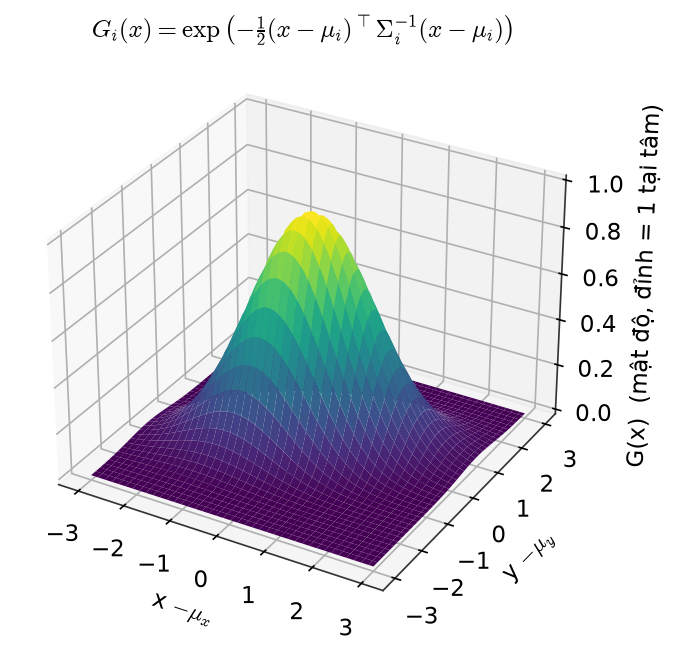
\includegraphics[width=0.4\linewidth]{ch2_gaussian_bump.png}
\end{center}
\end{frame}

% --- Slide: Tham số hoá hiệp phương sai ---
\begin{frame}{Tham số hoá hiệp phương sai: luôn xác định dương}
\scriptsize
Về mặt toán học, $\Sigma$ phải \textbf{đối xứng và xác định dương} mới là một ma trận hiệp phương sai hợp lệ (nếu
không, $G(x)$ ở trên có thể phát tán vô nghĩa). Nếu tối ưu trực tiếp $6$ số độc lập của $\Sigma$ bằng gradient descent,
rất dễ trong quá trình huấn luyện đi lệch khỏi vùng hợp lệ. Giải pháp của 3DGS là \textbf{phân rã} $\Sigma$ thành tích
của một ma trận quay và một ma trận scale:
\[
\boxed{\;\Sigma=RSS^\top R^\top\;},\qquad S=\mathrm{diag}(s_x,s_y,s_z),\qquad R=R\!\left(\frac{q}{\lVert q\rVert}\right)
\]
\begin{itemize}\itemsep1pt
    \item $S$: ma trận đường chéo với $s=\exp(\texttt{\_scaling})$ --- vì hàm mũ luôn dương, $s$ \textbf{tự động dương}
    với mọi giá trị thực của \texttt{\_scaling}, không cần ràng buộc (constraint) nào thêm khi tối ưu.
    \item $R$: ma trận quay $3\times3$ dựng từ quaternion $q$ đã \textbf{chuẩn hoá về độ dài 1} --- luôn là ma trận trực giao hợp lệ.
    \item Nhờ vậy $\Sigma=RSS^\top R^\top$ \textbf{tự động} đối xứng, xác định dương với \emph{bất kỳ} $s,q$ nào --- ta có
    thể tối ưu $s,q$ tự do bằng gradient descent mà không sợ vi phạm ràng buộc toán học.
    \item Về mặt hình học: ellipsoid của Gaussian có \textbf{bán trục theo mỗi hướng chính $= s_j$} (không phải trị riêng
    của $\Sigma$ --- trị riêng thực ra là $s_j^2$, vì $\Sigma$ là bình phương của $S$ sau khi quay).
\end{itemize}
\end{frame}

% --- Slide: Scale khởi tạo ---
\begin{frame}{Khởi tạo (1/2): scale ban đầu theo mật độ điểm SfM}
\scriptsize
Trước khi train, mỗi Gaussian được đặt \textbf{đúng tại vị trí} một điểm 3D thưa mà SfM/COLMAP đã tái dựng được từ các
ảnh input (\emph{sparse point cloud}). Nhưng vị trí thôi chưa đủ --- cần một \textbf{kích thước ban đầu hợp lý} cho mỗi
Gaussian: quá nhỏ thì để hở nhiều khoảng trống giữa các điểm, quá to thì các Gaussian chồng lấn nhau ngay từ đầu, làm
nhiễu tín hiệu học. Giải pháp: lấy khoảng cách tới các điểm lân cận làm thước đo mật độ cục bộ:
\[
\tilde s = \log\sqrt{\overline{d^2_{\mathrm{knn3}}}}
\]
tức là: với mỗi điểm, tính khoảng cách bình phương tới $3$ điểm gần nhất (knn3), lấy trung bình, rồi căn bậc hai --- ra
một ước lượng "khoảng cách điển hình giữa các điểm lân cận" tại vị trí đó. Lấy \texttt{log} vì scale được lưu và tối
ưu trong không gian log (nhất quán với $s=\exp(\texttt{\_scaling})$ ở slide trước). Kết quả: vùng point cloud dày đặc
(nhiều chi tiết hình học) sẽ có Gaussian khởi tạo \textbf{nhỏ}, vùng thưa sẽ có Gaussian khởi tạo \textbf{to} hơn ---
một cách tự nhiên để phủ kín cảnh mà không cần biết trước hình dạng vật thể.
\begin{center}
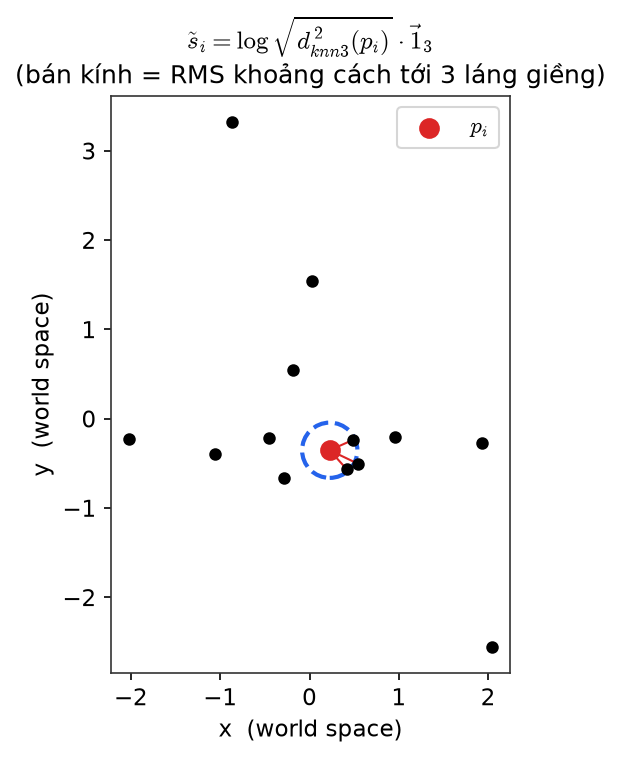
\includegraphics[width=0.42\linewidth]{ch1_scale_init.png}
\end{center}
\end{frame}

% --- Slide: Scene extent ---
\begin{frame}{Khởi tạo (2/2): scene extent --- thước đo "to/nhỏ" dùng xuyên suốt}
\scriptsize
Nhiều quyết định sau này trong ADC (Adaptive Density Control) cần biết "Gaussian này to hay nhỏ \textbf{so với quy mô
của cả cảnh}" --- ví dụ ngưỡng \texttt{percent\_dense}$\times$\texttt{extent} để phân biệt clone/split (sẽ nói ở phần
sau). Đại lượng dùng làm đơn vị đo lường này là \textbf{scene extent}, tính \textbf{một lần duy nhất} lúc khởi tạo:
\[
\boxed{\;\mathrm{extent}=1.1\cdot\max_v\lVert c_v-\bar c\rVert\;}
\]
với $c_v$ là vị trí của camera train thứ $v$, $\bar c$ là tâm trung bình của tất cả camera train. Nói cách khác, đây là
\textbf{bán kính} (nhân thêm hệ số an toàn $1.1$) của một khối cầu tưởng tượng bao quanh toàn bộ vị trí các camera ---
\textbf{không phải} đường chéo của hộp bao (bounding box) quanh point cloud như đôi khi bị hiểu nhầm. Vì cảnh thường
được quay quanh một đối tượng trung tâm, "bán kính vòng camera" là một ước lượng hợp lý cho kích thước tổng thể của cảnh.
\begin{center}
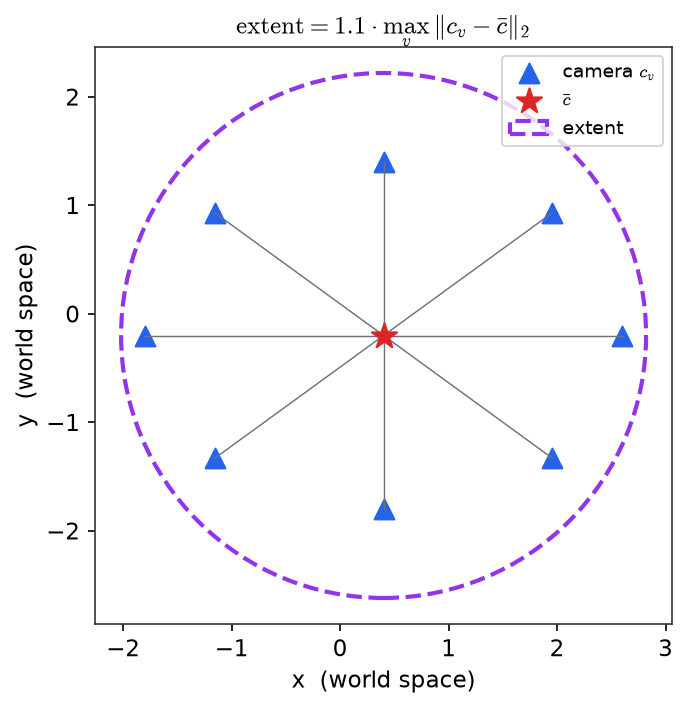
\includegraphics[width=0.42\linewidth]{ch1_extent.png}
\end{center}
\end{frame}

% --- Slide: Màu qua Spherical Harmonics ---
\begin{frame}{Màu phụ thuộc góc nhìn: hệ số Spherical Harmonics}
\scriptsize
Vật liệu thực tế (kim loại, nước, sứ bóng...) phản chiếu ánh sáng khác nhau tuỳ góc nhìn --- một màu RGB cố định không
mô phỏng được hiệu ứng này. 3DGS giải quyết bằng cách biểu diễn màu như một \textbf{hàm của hướng nhìn} $d$, khai triển
theo cơ sở \textbf{Spherical Harmonics} (SH) --- một họ hàm trực giao trên mặt cầu, tương tự chuỗi Fourier nhưng cho dữ
liệu định nghĩa trên hình cầu thay vì trên một đường thẳng:
\[
c(d)=\sum_{\ell=0}^{D}\sum_{m=-\ell}^{\ell} k_{\ell m}\,Y_{\ell}^{m}(d)
\]
mỗi Gaussian lưu các \textbf{hệ số} $k_{\ell m}$ (học được), không lưu trực tiếp màu.
\begin{itemize}\itemsep1pt
    \item Hệ số bậc $0$ ($\ell=0$, gọi là \textbf{hệ số DC}) chính là \textbf{màu trung bình theo mọi góc nhìn}: khởi tạo
    $k_{00}=\mathrm{RGB2SH}(c)=(c-0.5)/C_0$ với hằng số chuẩn hoá $C_0=\tfrac{1}{2\sqrt\pi}\approx0.282$.
    \item Các hệ số bậc cao hơn ($\ell\ge1$) mã hoá \textbf{độ thay đổi màu theo hướng nhìn} --- càng nhiều bậc, hiệu ứng
    phản chiếu/specular càng chi tiết, nhưng cũng càng nhiều tham số phải học.
    \item Tổng số hệ số cần học nếu dùng tới bậc $D$: $(D+1)^2$ hệ số cho mỗi kênh màu; với $D=3$ (giá trị dùng phổ biến)
    là $16$ hệ số/kênh $\times3$ kênh $=48$ số ($3$ số DC $+$ $45$ số bậc cao, tên biến \texttt{f\_rest}).
\end{itemize}
\begin{center}
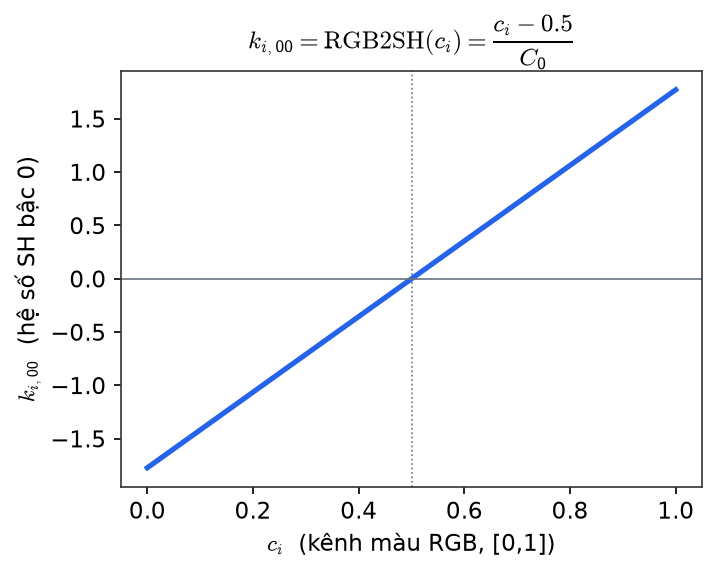
\includegraphics[width=0.30\linewidth]{ch1_rgb2sh.png}
\end{center}
\end{frame}

% --- Slide: Lịch tăng bậc SH ---
\begin{frame}{Lịch tăng bậc SH: vì sao không học bậc cao ngay từ đầu?}
\scriptsize
Học ngay $48$ hệ số SH từ những iteration đầu tiên, khi vị trí/hình dạng Gaussian còn rất chưa ổn định, dễ làm mô hình
"khớp" (overfit) vào những biến thiên màu do \textbf{sai vị trí hình học} gây ra, chứ không phải phản chiếu thật ---
gây nhiễu và bất ổn cho quá trình tối ưu. Giải pháp: \textbf{tăng bậc SH dần dần}, để hình học ổn định trước, chi tiết
phản chiếu học sau. Trong code (\texttt{train.py:216--217}):
\[
\texttt{if iteration \% 1 == 0: gaussians.oneupSHdegree()}
\]
tức bậc \textbf{tăng thêm 1 sau mỗi iteration}, cho tới khi chạm bậc tối đa $D_{\max}=3$ --- nghĩa là chỉ sau \textbf{3
iteration đầu tiên} của cả quá trình train ($30\,000$ iteration), toàn bộ Gaussian đã dùng bậc SH tối đa. Đây là một
điểm dễ hiểu lầm: nhiều tài liệu khác về 3DGS mô tả lịch tăng bậc là "mỗi vài nghìn iteration tăng 1 bậc" --- con số đó
\textbf{không khớp} với đoạn code thực tế của chính pipeline này.
\begin{center}
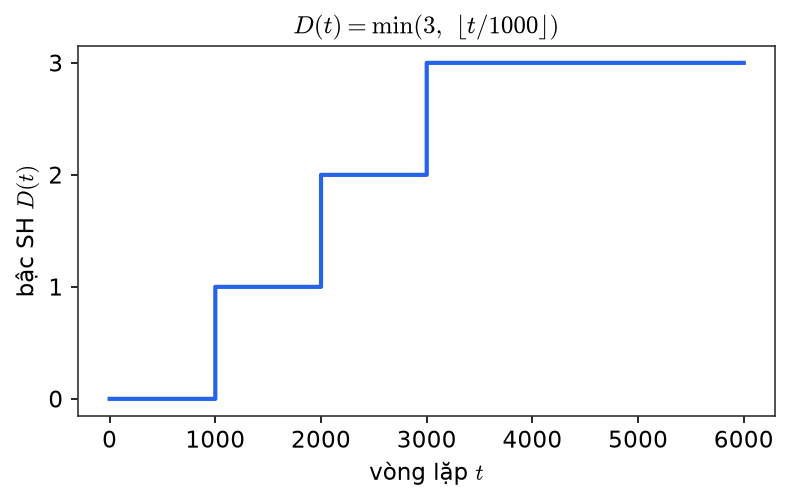
\includegraphics[width=0.42\linewidth]{ch2_sh_degree_schedule.png}
\end{center}
\end{frame}
   % Slide 1-4   Bìa/agenda, Động lực, 3D Gaussian là gì
% ===== FILE 2/9: Pinhole, EWA projection, Compact box, Trường alpha, Alpha blending, Transmittance decay =====

% --- Slide: Chiếu camera pinhole ---
\begin{frame}{Chiếu điểm 3D lên màn hình: mô hình pinhole}
\scriptsize
Để vẽ một Gaussian 3D lên ảnh 2D, bước đầu tiên là biết \textbf{tâm của nó rơi vào pixel nào}. Camera pinhole (mô hình
camera tiêu chuẩn trong thị giác máy tính) chiếu một điểm $(x,y,z)$ trong hệ toạ độ camera thành pixel $(u,v)$ theo
phép chiếu phối cảnh cổ điển:
\[
\boxed{\;u=f_x\frac{x}{z}+c_x,\qquad v=f_y\frac{y}{z}+c_y\;}
\]
với $(f_x,f_y)$ là tiêu cự tính theo đơn vị pixel (phụ thuộc độ phân giải ảnh và góc nhìn của camera), $(c_x,c_y)$ là
\textbf{điểm chính} (thường là chính giữa ảnh, $W/2,H/2$).
\begin{itemize}\itemsep1pt
    \item Đây là phép chiếu \textbf{phi tuyến} vì có phép chia cho $z$ (độ sâu) --- vật càng xa càng nhỏ lại, đúng như
    cảm nhận thị giác thông thường.
    \item Vấn đề: Gaussian không phải một điểm mà là cả một \textbf{ellipsoid 3D} --- phép chiếu phi tuyến của cả một
    khối hình không cho ra một ellipse đẹp một cách chính xác. Giải pháp thực dụng: \textbf{tuyến tính hoá cục bộ} quanh
    tâm Gaussian bằng ma trận Jacobian $J$ (đạo hàm riêng của phép chiếu tại đúng điểm đó):
\end{itemize}
\[
J=\begin{pmatrix} f_x/z & 0 & -f_x x/z^2\\ 0 & f_y/z & -f_y y/z^2\end{pmatrix}
\]
Ma trận $J$ này sẽ được dùng lại ở \textbf{cả hai nơi}: chiếu hiệp phương sai sang 2D ngay sau đây, và chiếu trục
Gaussian của cơ chế SADGS về sau.
\begin{center}
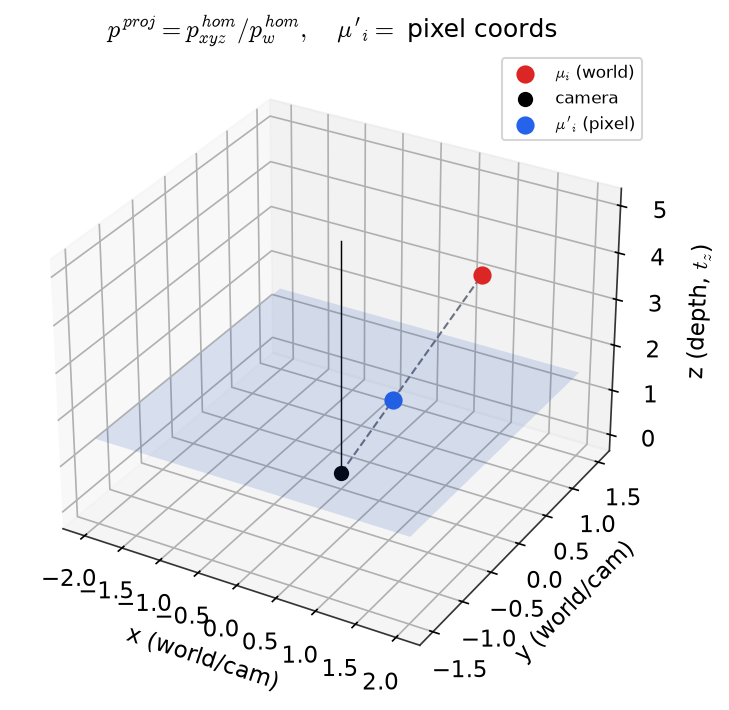
\includegraphics[width=0.34\linewidth]{ch3_pinhole_projection.png}
\end{center}
\end{frame}

% --- Slide: EWA covariance projection ---
\begin{frame}{EWA splatting: chiếu ellipsoid 3D thành ellipse 2D}
\scriptsize
Dùng Jacobian $J$ ở slide trước, ta xấp xỉ tuyến tính phép chiếu của toàn bộ hiệp phương sai $\Sigma$ (kỹ thuật
\emph{Elliptical Weighted Average}, Zwicker et al. 2001 --- nền tảng toán học cho mọi hệ splatting hiện đại):
\[
\boxed{\;\Sigma' = \big[\,J\,W\,\Sigma\,W^\top J^\top\,\big]_{2\times2} + \kappa\, I\;}
\]
$W$ là ma trận quay world$\to$camera; $[\cdot]_{2\times2}$ nghĩa là chỉ giữ lại khối $2{\times}2$ trên-trái của kết quả
(bỏ chiều depth, vì ta chỉ cần ellipse trên mặt phẳng ảnh).
\begin{itemize}\itemsep1pt
    \item \textbf{Vì sao cần $+\kappa I$?} Khi Gaussian ở rất xa camera hoặc bị nhìn gần như từ cạnh, ellipse chiếu ra
    có thể suy biến thành một đường gần như không có bề rộng --- gây chia cho $0$ và alias (răng cưa). Cộng thêm
    $\kappa I$ đảm bảo ellipse luôn rộng \textbf{ít nhất khoảng 1 pixel} theo mọi hướng --- một bộ lọc low-pass đơn giản, \textbf{luôn được áp dụng}, không phải tuỳ chọn.
    \item Trong CUDA kernel thực tế của repo này (\texttt{cuda\_rasterizer/forward.cu:113--117}), $\kappa=0.1$ --- khác
    với con số $0.3$ vẫn thường thấy trong một số tài liệu 3DGS khác.
    \item Vì "phồng" hiệp phương sai làm sai lệch tổng năng lượng của Gaussian, renderer nhân bù ngược một \textbf{hệ số
    hiệu chỉnh} $\mathrm{coef}=\sqrt{\det\Sigma'_{\text{trước}}/\det\Sigma'_{\text{sau}}}$ vào $\alpha$ để giữ năng lượng gần đúng.
\end{itemize}
\begin{center}
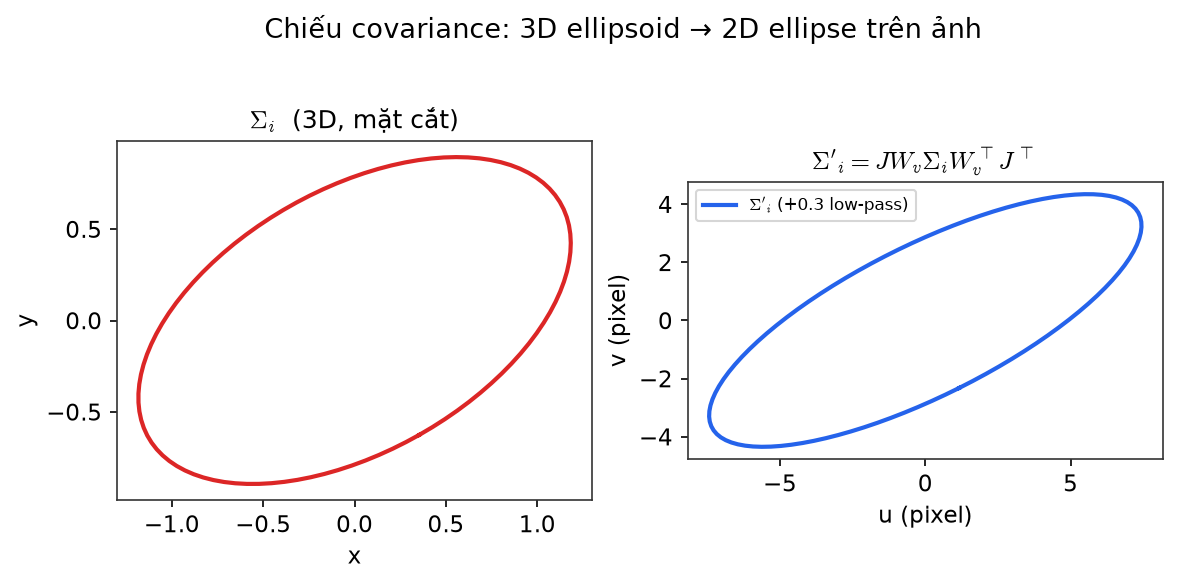
\includegraphics[width=0.34\linewidth]{ch3_ewa_projection.png}
\end{center}
\end{frame}

% --- Slide: Compact box ---
\begin{frame}{Compact box: xác định Gaussian phủ những tile nào}
\scriptsize
Sau khi có ellipse 2D, renderer cần biết nó \textbf{chạm tới những tile $16\times16$ pixel nào} trên màn hình --- đây
là bước quyết định renderer nhanh hay chậm (Gaussian chạm càng nhiều tile, càng tốn công xử lý). Repo này dùng kỹ thuật
\textbf{SnugBox} (\texttt{cuda\_rasterizer/auxiliary.h:313--340}, kỹ thuật kế thừa từ dòng nghiên cứu Taming/Speedy-Splat,
\textbf{không phải điểm mới của SADGS}) --- thay vì bao Gaussian bằng một hình vuông cố định $3\sigma$ như 3DGS gốc,
SnugBox dựng một hộp bao \textbf{khít sát theo đúng hình dạng ellipse thật}, tại ngưỡng nơi $\alpha\cdot G=1/255$ (dưới
mức này coi như không nhìn thấy được nữa), có thể siết chặt hơn nữa bằng một hệ số điều chỉnh \texttt{mult}:
\[
\boxed{\;t=\texttt{mult}\cdot 2\ln(255\,\alpha)\;}\qquad(\texttt{mult}=0.7\text{ mặc định}, \texttt{arguments/\_\_init\_\_.py:114})
\]
\begin{itemize}\itemsep1pt
    \item $\texttt{mult}=1$: khớp đúng ngưỡng $1/255$ gốc (SnugBox nguyên bản, không cắt xén thêm gì).
    \item $\texttt{mult}<1$: cắt \textbf{sớm hơn} $1/255$ --- ngưỡng cắt thật trở thành $\alpha_{\text{biên}}=\sigma_o(255\sigma_o)^{-\texttt{mult}}>1/255$, nghĩa là đánh đổi một phần đuôi Gaussian \emph{vẫn còn nhìn thấy được} để lấy tốc độ (ít tile hơn/Gaussian $\Rightarrow$ ít công tính hơn).
\end{itemize}
\begin{center}
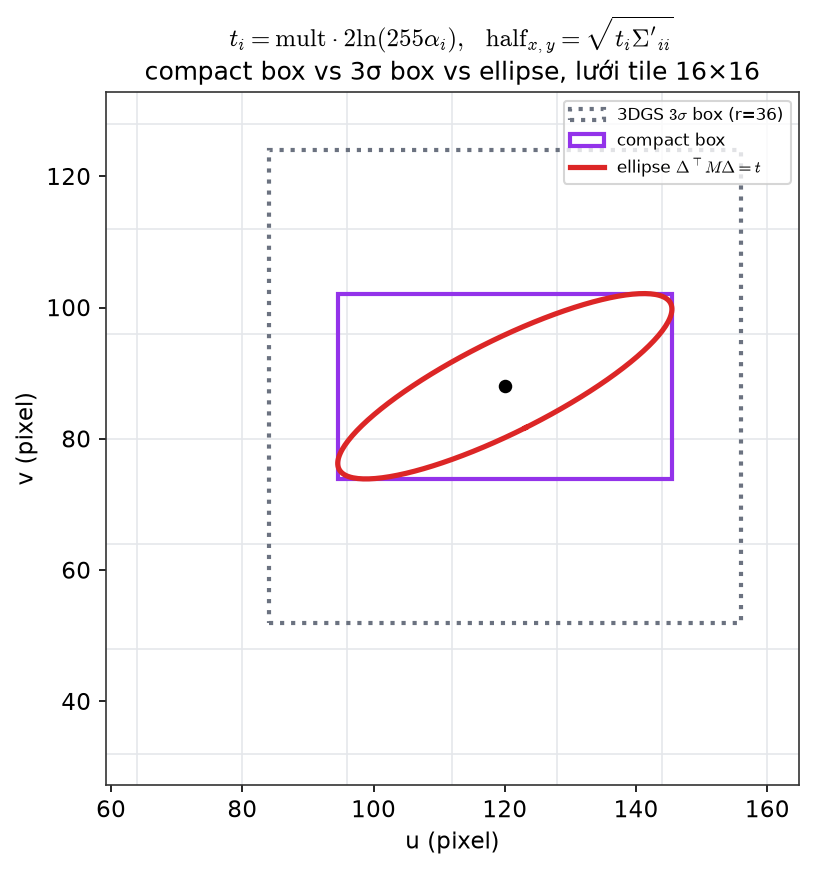
\includegraphics[width=0.30\linewidth]{ch3_compact_box.png}
\end{center}
\end{frame}

% --- Slide: Trường alpha ---
\begin{frame}{Trường alpha: mỗi Gaussian che phủ pixel bao nhiêu?}
\scriptsize
Một Gaussian không "đặc" đều --- độ che phủ giảm dần từ tâm ra biên theo đúng hàm $G(x)$. Tại một pixel cụ thể $x$
trên màn hình, độ mờ đục hiệu dụng của Gaussian thứ $n$ là:
\[
\boxed{\;\alpha_n(x)=\min\big(0.99,\ \alpha_n\, G_n(x)\big)\;}
\]
\begin{itemize}\itemsep1pt
    \item $\alpha_n$ (tham số học được, cố định cho cả Gaussian) nhân với $G_n(x)$ (giá trị hàm Gaussian 2D đã chiếu,
    \textbf{thay đổi theo từng pixel} $x$ --- cao nhất tại tâm ellipse, giảm dần ra ngoài).
    \item Chặn trên $0.99$ (không phải $1.0$): tránh một Gaussian duy nhất "che kín hoàn toàn" khiến gradient của mọi
    Gaussian phía sau nó biến mất hẳn --- luôn để lại một khe hở rất nhỏ cho tín hiệu gradient lan truyền.
    \item Đây chính là đại lượng $\alpha_n(x)$ sẽ được dùng trong công thức alpha blending ở slide tiếp theo --- lưu ý nó
    phụ thuộc pixel, khác với $\alpha_n$ hằng số của riêng Gaussian.
\end{itemize}
\begin{center}
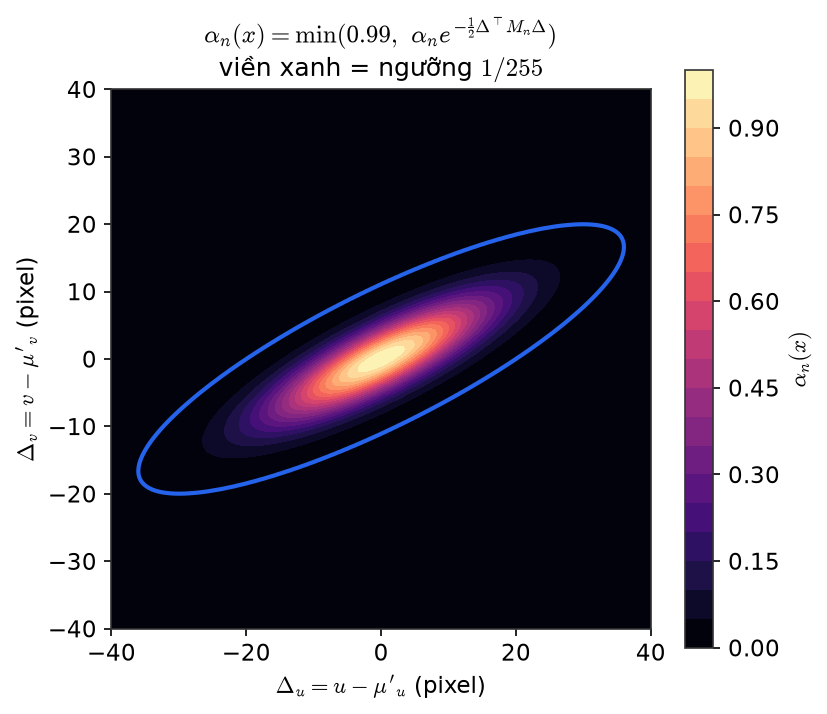
\includegraphics[width=0.36\linewidth]{ch4_alpha_field.png}
\end{center}
\end{frame}

% --- Slide: Alpha blending ---
\begin{frame}{Alpha blending: trộn nhiều lớp Gaussian theo thứ tự trước-sau}
\scriptsize
Tại một pixel, có thể có \textbf{nhiều Gaussian} chồng lên nhau theo chiều sâu. Màu cuối cùng là kết quả trộn tuần tự
từ Gaussian gần camera nhất ra xa nhất (front-to-back alpha blending, giống cách vẽ các lớp trong suốt chồng lên nhau):
\[
\boxed{\;C(x)=\sum_{n} c_n\,\alpha_n(x)\,T_n(x) \;+\; T_{\text{final}}(x)\,C_{bg}\;},\qquad
T_n(x)=\prod_{j<n}\big(1-\alpha_j(x)\big)
\]
\begin{itemize}\itemsep1pt
    \item $T_n$ (\textbf{transmittance}): tỉ lệ ánh sáng \emph{còn lại}, chưa bị các Gaussian phía trước "hấp thụ" ---
    Gaussian thứ $n$ chỉ đóng góp đúng phần ánh sáng nó nhận được sau khi đã đi qua $n-1$ lớp trước nó.
    \item Số hạng $T_{\text{final}}C_{bg}$ (màu \textbf{nền}) là bắt buộc, không được bỏ qua: nếu tổng $\alpha_n(x)$ dọc
    một tia không phủ hết $1$ (ví dụ vùng thưa Gaussian), phần còn thiếu phải được lấp bằng màu nền, nếu không ảnh sẽ bị
    tối sai so với thực tế.
\end{itemize}
\begin{center}
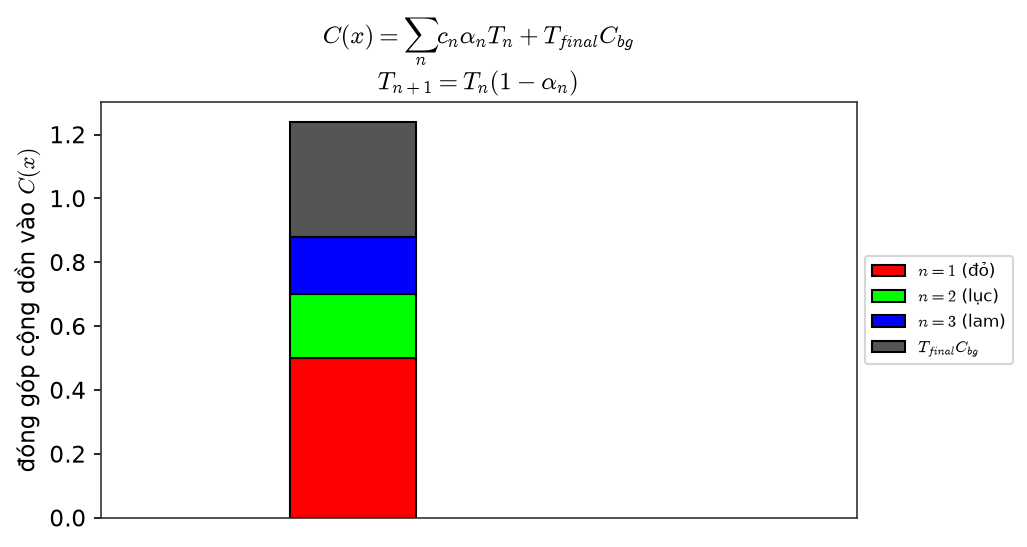
\includegraphics[width=0.36\linewidth]{ch4_alpha_blend_stack.png}
\end{center}
\end{frame}

% --- Slide: Transmittance decay & early stop ---
\begin{frame}{Transmittance suy giảm: cơ sở cho việc dừng sớm}
\scriptsize
Vì $T_n=\prod_{j<n}(1-\alpha_j(x))$ là tích của các thừa số $\le1$, $T_n$ \textbf{giảm dần theo cấp số nhân} khi đi qua
ngày càng nhiều lớp Gaussian (đặc biệt rõ khi từng $\alpha_j(x)$ đều đáng kể). Sau một số lớp đủ nhiều, $T_n$ trở nên
cực nhỏ --- các Gaussian tiếp theo dù có màu gì cũng gần như \textbf{không còn ảnh hưởng} tới $C(x)$ nữa vì bị nhân với
một hệ số gần $0$.
\begin{itemize}\itemsep1pt
    \item Renderer tận dụng điều này để \textbf{dừng sớm} (early termination): ngay khi $T\cdot(1-\alpha)<10^{-4}$ tại
    một pixel, ngừng xử lý thêm Gaussian cho pixel đó --- tiết kiệm đáng kể thời gian tính toán mà hầu như không ảnh
    hưởng chất lượng ảnh (sai số dưới ngưỡng nhận biết được).
    \item Đây cũng là lý do vì sao \textbf{thứ tự depth} (Gaussian nào gần camera hơn) rất quan trọng: nếu sắp sai thứ
    tự, dừng sớm có thể bỏ lỡ một Gaussian đáng lẽ vẫn còn đóng góp đáng kể.
\end{itemize}
\begin{center}
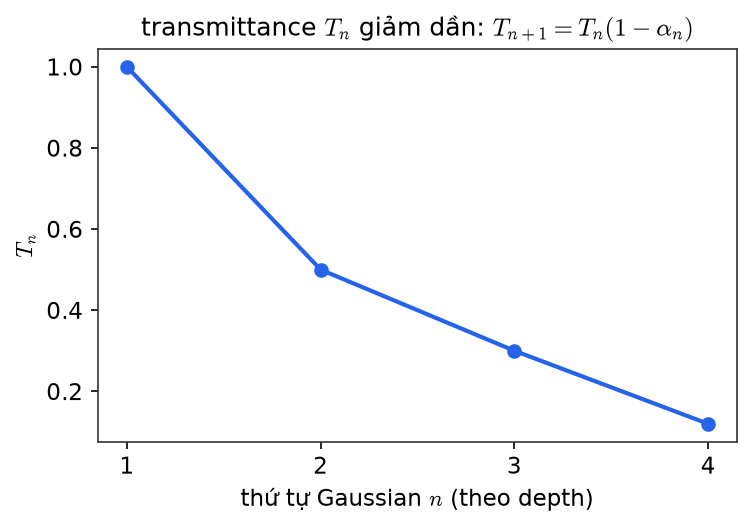
\includegraphics[width=0.36\linewidth]{ch4_transmittance_decay.png}
\end{center}
\end{frame}
   % Slide 5-8   Hiệp phương sai, Màu SH, Pipeline render, EWA splatting
% ===== FILE 3/9: Tile rasterizer, Loss, PSNR, SSIM, Score tổng hợp =====

% --- Slide: Tile-based rasterizer ---
\begin{frame}{Kiến trúc rasterizer theo tile: vì sao render nhanh}
\scriptsize
Với hàng triệu Gaussian và hàng triệu pixel, việc lặp "cho mỗi pixel, quét qua mọi Gaussian" là bất khả thi về tốc độ.
3DGS giải quyết bằng kiến trúc \textbf{song song hoá theo tile}, chia màn hình thành các ô $16\times16$ pixel:
\begin{enumerate}\itemsep2pt
    \item \textbf{Xác định phạm vi:} với mỗi Gaussian, dùng compact box (slide trước) để biết nó phủ tới những tile
    nào $\Rightarrow$ sinh ra các cặp khoá $(\text{chỉ số tile}, \text{độ sâu})$ --- một Gaussian phủ nhiều tile thì sinh
    nhiều cặp khoá, mỗi cặp ứng với một tile.
    \item \textbf{Sắp xếp một lần duy nhất:} toàn bộ danh sách cặp khoá được sắp theo $(\text{tile}, \text{depth})$ ---
    đây là bước tốn kém nhất về mặt lý thuyết, nhưng chỉ thực hiện \textbf{một lần cho cả khung hình}, không phải một
    lần riêng cho từng pixel như cách làm ngây thơ.
    \item \textbf{Xử lý song song theo tile:} mỗi \emph{thread block} trên GPU phụ trách đúng một tile; vì danh sách đã
    sắp sẵn theo depth, mỗi thread chỉ cần blend tuần tự (công thức alpha blending, slide trước) theo đúng thứ tự, dừng
    sớm khi $T$ đủ nhỏ.
\end{enumerate}
\textbf{Kết quả:} tổng chi phí gần với $O(N\cdot K)$, với $K$ là số tile trung bình mà mỗi Gaussian chạm tới (bị chi
phối trực tiếp bởi \texttt{mult} của compact box) --- thay vì $O(N\cdot H\cdot W)$ nếu phải quét toàn ảnh cho mỗi
Gaussian. Đây là lý do cốt lõi giúp 3DGS render \textbf{thời gian thực}.
\end{frame}

% --- Slide: Hàm mất mát ---
\begin{frame}{Hàm mất mát: so khớp ảnh render với ảnh thật}
\scriptsize
Sau khi render ra ảnh $I_{\text{render}}$, cần một hàm đo "khác biệt" với ảnh thật $I_{gt}$ để lấy gradient huấn luyện.
Trong repo này (\texttt{train.py:256--259}):
\[
\boxed{\;\mathcal{L} = (1-\lambda_{\text{dssim}})\,L_1 + \lambda_{\text{dssim}}\,(1-\mathrm{SSIM}) + \lambda_{L2}\,L_2\;}
\]
với $\lambda_{\text{dssim}}=0.2$, $\lambda_{L2}=2.0$ --- so với 3DGS gốc (chỉ có hai số hạng đầu), bản này \textbf{cộng
thêm} một số hạng $L_2$ (bình phương sai số theo pixel, \texttt{utils/loss\_utils.py:25}).
\begin{itemize}\itemsep1pt
    \item $L_1=\overline{|I_{\text{render}}-I_{gt}|}$: ổn định, ít bị kéo lệch bởi vài pixel ngoại lệ (outlier) --- một
    vài pixel sai rất nhiều (do noise, occlusion...) không làm gradient tổng thể "hoảng loạn".
    \item $\mathrm{SSIM}$ (Structural Similarity, cửa sổ Gaussian $11\times11$, $\sigma=1.5$): so khớp \textbf{cấu trúc
    cục bộ} --- độ tương phản, độ chói theo từng vùng nhỏ --- gần với cảm nhận thị giác con người hơn so sánh từng pixel riêng lẻ.
    \item $L_2$ (bình phương): phạt \textbf{nặng hơn} với sai số lớn, giúp mô hình hội tụ nhanh ở giai đoạn đầu khi ảnh
    render còn rất khác ảnh thật.
    \item \textbf{Ghi chú quan trọng:} \texttt{loss\_utils.py} còn định nghĩa hai hàm \texttt{tone\_curve\_loss} và
    \texttt{frequency\_loss} (dựa trên structure tensor sẽ nói ở phần SADGS) --- nhưng \textbf{không có dòng nào trong
    \texttt{train.py} gọi tới hai hàm này}. Đây là \emph{dead code}: tồn tại trong file nhưng không ảnh hưởng gì tới
    loss thật sự đang được tối ưu.
\end{itemize}
\begin{center}
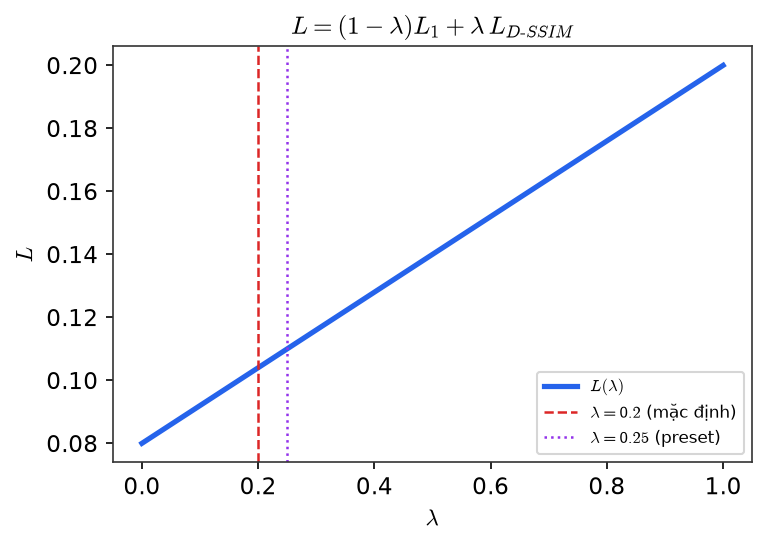
\includegraphics[width=0.34\linewidth]{ch5_loss_mix.png}
\end{center}
\end{frame}

% --- Slide: PSNR ---
\begin{frame}{Đánh giá chất lượng (1/3): PSNR}
\scriptsize
Sau khi train xong, cần các chỉ số \textbf{độc lập với loss} để đánh giá khách quan chất lượng render trên tập test
(ảnh chưa dùng để train). Chỉ số đầu tiên và đơn giản nhất là \textbf{PSNR} (Peak Signal-to-Noise Ratio):
\[
\mathrm{PSNR}=10\log_{10}\!\left(\frac{1}{\mathrm{MSE}}\right)\quad\text{(dB, với ảnh chuẩn hoá về }[0,1]\text{)}
\]
\begin{itemize}\itemsep1pt
    \item PSNR càng \textbf{cao} nghĩa là sai số bình phương trung bình theo pixel càng \textbf{thấp} --- là thang đo
    logarit nên chênh lệch vài dB đã tương ứng với chênh lệch sai số đáng kể.
    \item \textbf{Hạn chế:} PSNR đối xử với mọi pixel như nhau, không phân biệt "sai ở vùng chi tiết phức tạp" hay "sai ở
    vùng phẳng đơn giản" --- hai ảnh có cùng PSNR có thể trông rất khác nhau về mặt cảm nhận thị giác (một ảnh mờ đều,
    một ảnh có vài vệt lỗi rõ rệt nhưng phần còn lại rất sắc nét).
    \item Vì hạn chế này, PSNR thường được báo cáo \textbf{cùng với} SSIM và LPIPS (hai slide tiếp theo), không dùng một mình.
\end{itemize}
\begin{center}
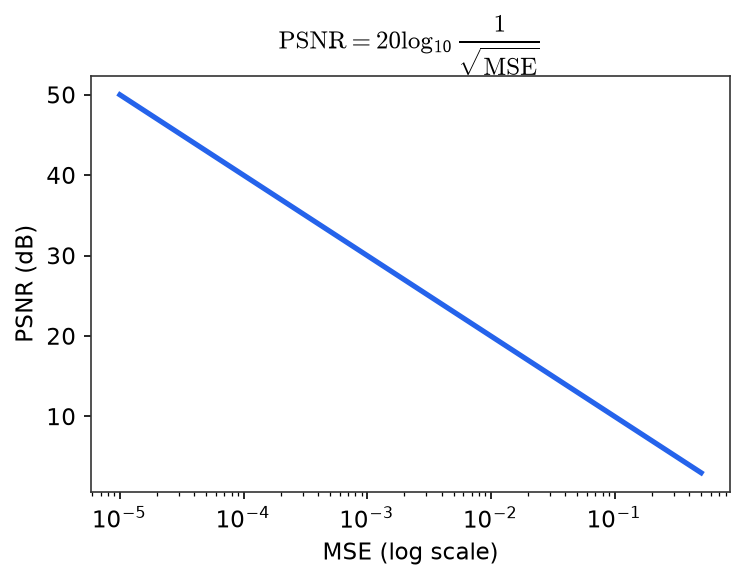
\includegraphics[width=0.36\linewidth]{ch5_psnr.png}
\end{center}
\end{frame}

% --- Slide: SSIM ---
\begin{frame}{Đánh giá chất lượng (2/3): SSIM}
\scriptsize
\textbf{SSIM} (Structural Similarity Index) --- cùng công thức đã dùng làm một phần của loss (slide trước) --- nhưng ở
đây dùng để \textbf{đánh giá}, không phải để lấy gradient. So sánh ảnh theo \textbf{cửa sổ trượt cục bộ} (Gaussian
$11\times11$, $\sigma=1.5$), kết hợp ba thành phần: độ chói (luminance), độ tương phản (contrast), và cấu trúc
(structure) giữa hai ảnh trong mỗi cửa sổ.
\begin{itemize}\itemsep1pt
    \item Giá trị nằm trong $[-1,1]$ (thường báo cáo trong $[0,1]$ với ảnh tự nhiên), $1$ là khớp hoàn hảo.
    \item Vì so sánh theo \textbf{vùng cục bộ} thay vì từng pixel riêng lẻ, SSIM nhạy với sai lệch về \textbf{cấu trúc}
    (đường nét, hoạ tiết bị mờ/lệch) hơn là sai lệch nhỏ về độ sáng tổng thể --- gần với cách mắt người đánh giá "ảnh này
    có giống ảnh kia không" hơn PSNR thuần.
    \item Trong 3DGS, SSIM đóng vai trò \textbf{kép}: vừa là một phần của hàm loss lúc train (khuyến khích khớp cấu
    trúc), vừa là chỉ số đánh giá lúc test.
\end{itemize}
\begin{center}
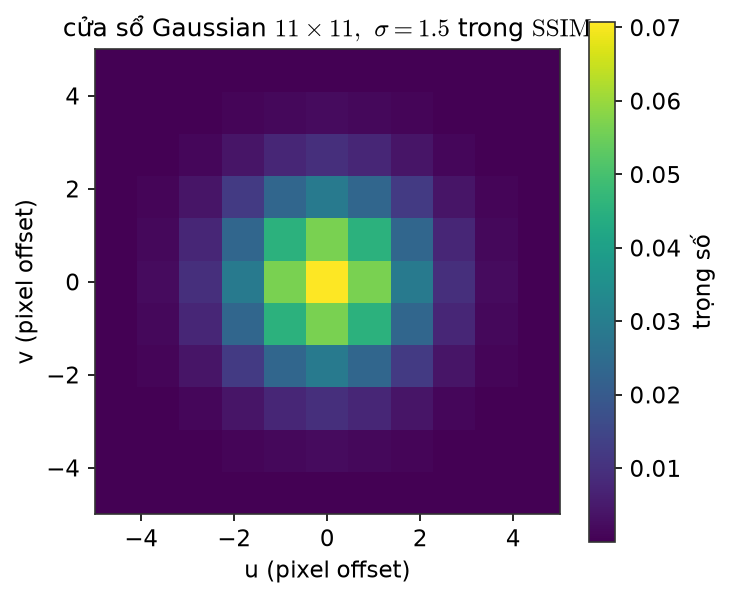
\includegraphics[width=0.36\linewidth]{ch5_ssim_window.png}
\end{center}
\end{frame}

% --- Slide: Score tổng hợp ---
\begin{frame}{Đánh giá chất lượng (3/3): kết hợp nhiều chỉ số}
\scriptsize
Ba chỉ số PSNR, SSIM, và \textbf{LPIPS} (Learned Perceptual Image Patch Similarity --- khoảng cách giữa hai ảnh đo
trong không gian đặc trưng của một mạng CNN đã huấn luyện trước trên dữ liệu thị giác con người) đo những khía cạnh
\textbf{khác nhau và bổ sung cho nhau}:
\begin{itemize}\itemsep1pt
    \item PSNR: sai số pixel thô, dễ tính, dễ hiểu, nhưng ít tương quan với cảm nhận thị giác.
    \item SSIM: cấu trúc cục bộ, tương quan tốt hơn với cảm nhận, nhưng vẫn là một công thức toán học tường minh, không "học" từ dữ liệu thị giác người.
    \item LPIPS: học trực tiếp từ dữ liệu đánh giá của con người, bắt được các khác biệt "nhìn thấy rõ" mà PSNR/SSIM có
    thể bỏ sót (ví dụ: một chi tiết bị làm mờ nhẹ nhưng vẫn giữ đúng cấu trúc trung bình).
    \item Không chỉ số nào là "đủ một mình" --- một báo cáo kết quả nghiêm túc nên nêu \textbf{cả ba}, kèm rõ scene,
    checkpoint (số iteration), và cấu hình đo, để tránh so sánh khập khiễng giữa các thiết lập khác nhau.
\end{itemize}
\begin{center}
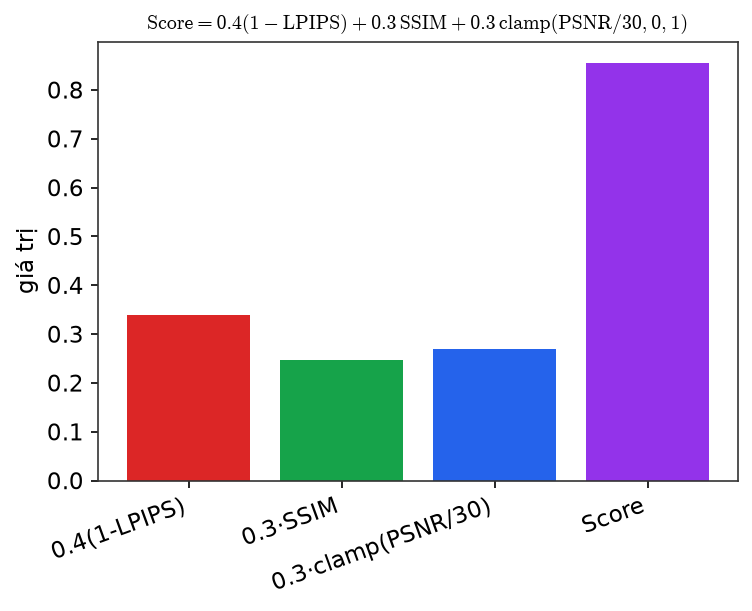
\includegraphics[width=0.36\linewidth]{ch5_score_decomp.png}
\end{center}
\end{frame}
   % Slide 9-12  Compact Box, Alpha blending, Tổng kết render, Loss

\section{Training \& Gradient}
% ===== FILE 4/9: Lan truyền gradient, Tích luỹ gradient, Triệt tiêu gradient, ADC tổng quan, Clone =====

% --- Slide: Lan truyền gradient ---
\begin{frame}{Lan truyền gradient: từ loss ngược về từng tham số Gaussian}
\scriptsize
Toàn bộ pipeline vừa trình bày --- chiếu, EWA, alpha blending --- là một chuỗi phép toán \textbf{khả vi} (differentiable),
nên PyTorch có thể tự động tính đạo hàm của loss theo bất kỳ tham số nào bằng quy tắc chuỗi (chain rule):
\[
\frac{\partial\mathcal{L}}{\partial\theta}=\sum_{x}\frac{\partial\mathcal{L}}{\partial C(x)}\cdot\frac{\partial C(x)}{\partial\theta},
\qquad \theta\in\{\mu, s, q, \alpha, k_{\ell m}\}
\]
\begin{itemize}\itemsep1pt
    \item Với mỗi pixel $x$ mà một Gaussian có góp mặt, đạo hàm $\partial C(x)/\partial\theta$ lan ngược qua đúng chuỗi
    các bước đã tính thuận: alpha blending $\to \alpha_n(x)=\min(0.99,\alpha_nG_n(x)) \to G_n(x) \to \Sigma',\mu'$ (EWA)
    $\to \Sigma,\mu$ (không gian 3D) $\to s,q$ (tham số hoá hiệp phương sai).
    \item \textbf{Quan sát then chốt cho phần sau:} gradient của \textbf{vị trí chiếu} $\partial\mathcal{L}/\partial\mu'$
    (trong không gian màn hình) có xu hướng \textbf{tập trung mạnh ở vùng biên} của Gaussian trong ảnh --- nơi cường độ
    ảnh thay đổi nhanh nhất --- chứ không rải đều khắp cả footprint. Điều này hợp lý về trực giác: ở vùng phẳng, sai một
    chút vị trí Gaussian không ảnh hưởng nhiều tới màu render; ở biên/cạnh sắc, một sai lệch nhỏ về vị trí gây thay đổi
    màu đáng kể ngay lập tức.
    \item Chính đại lượng $\partial\mathcal{L}/\partial\mu'$ này là \textbf{tín hiệu} mà Adaptive Density Control dùng để
    quyết định "Gaussian này có đang thiếu/thừa hình học không" (2 slide sau) --- nhưng bản thân tín hiệu này cũng ẩn
    chứa một vấn đề tinh vi, sẽ nói ngay sau đây.
\end{itemize}
\begin{center}
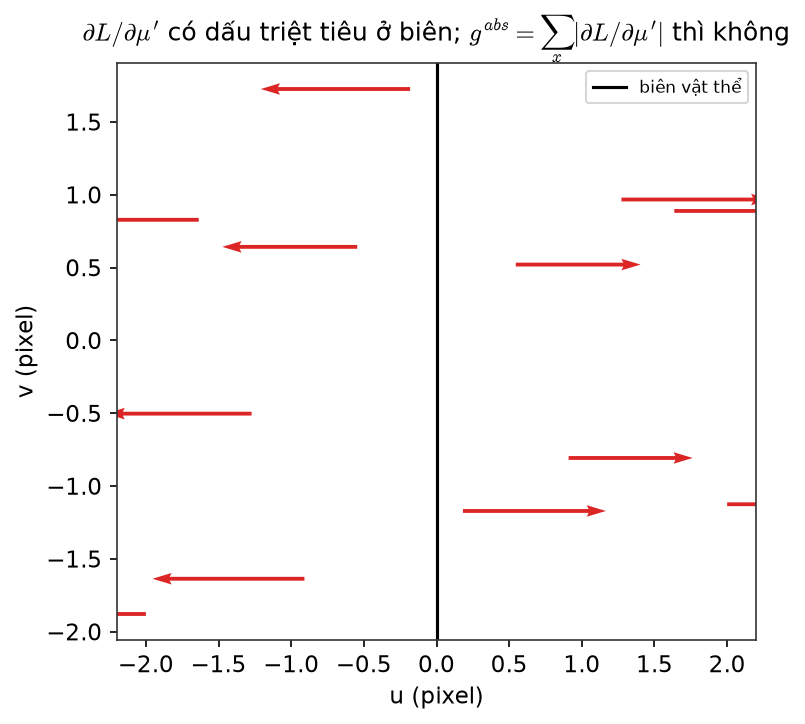
\includegraphics[width=0.36\linewidth]{ch6_edge_gradient.png}
\end{center}
\end{frame}

% --- Slide: Tích luỹ gradient view-space ---
\begin{frame}{Tích luỹ gradient qua nhiều view: lấy CHUẨN trước, cộng sau}
\scriptsize
Một Gaussian thường được camera train nhìn thấy từ \textbf{nhiều góc khác nhau} trong một epoch (một lượt qua hết mọi
camera). Để quyết định densify, cần tổng hợp gradient thu được từ tất cả các lần render đó. Hàm
\texttt{add\_densification\_stats} (\texttt{scene/gaussian\_model.py:1054--1057}) làm điều này như sau:
\[
\boxed{\;\texttt{xyz\_gradient\_accum}_i \mathrel{+}= \big\lVert \nabla_{\mu'_i}\mathcal{L}\big\rVert_{2}\;},\qquad
\bar g_i=\frac{\texttt{xyz\_gradient\_accum}_i}{\texttt{denom}_i}
\]
với \texttt{denom}$_i$ là số lần Gaussian $i$ được nhìn thấy (và cộng dồn) tính tới thời điểm đó.
\begin{itemize}\itemsep1pt
    \item \textbf{Điểm mấu chốt cần nhớ:} phép \textbf{lấy chuẩn} $\lVert\cdot\rVert$ diễn ra \textbf{ngay tại mỗi lần
    render} (mỗi view), \textbf{trước khi} cộng dồn qua \texttt{denom} --- không phải cộng các \emph{vector} gradient
    của nhiều view lại với nhau rồi mới lấy chuẩn một lần ở cuối.
    \item Hệ quả trực tiếp: vì mỗi số hạng được cộng vào \texttt{xyz\_gradient\_accum} luôn là một \textbf{số không âm}
    (chuẩn của một vector luôn $\ge0$), gradient từ các view \textbf{khác nhau tuyệt đối không thể triệt tiêu lẫn nhau}
    trong phép cộng này.
    \item Repo này còn tích luỹ song song một kênh \textbf{trị tuyệt đối} riêng biệt, \texttt{xyz\_gradient\_accum\_abs}
    --- dùng làm tín hiệu cho ngưỡng \texttt{grad\_abs\_thresh} khi quyết định \textbf{split}, tách biệt hoàn toàn với
    ngưỡng \texttt{grad\_thresh} dùng cho \textbf{clone}. Vì sao cần tới hai kênh gradient khác nhau --- xem slide kế tiếp.
\end{itemize}
\begin{center}
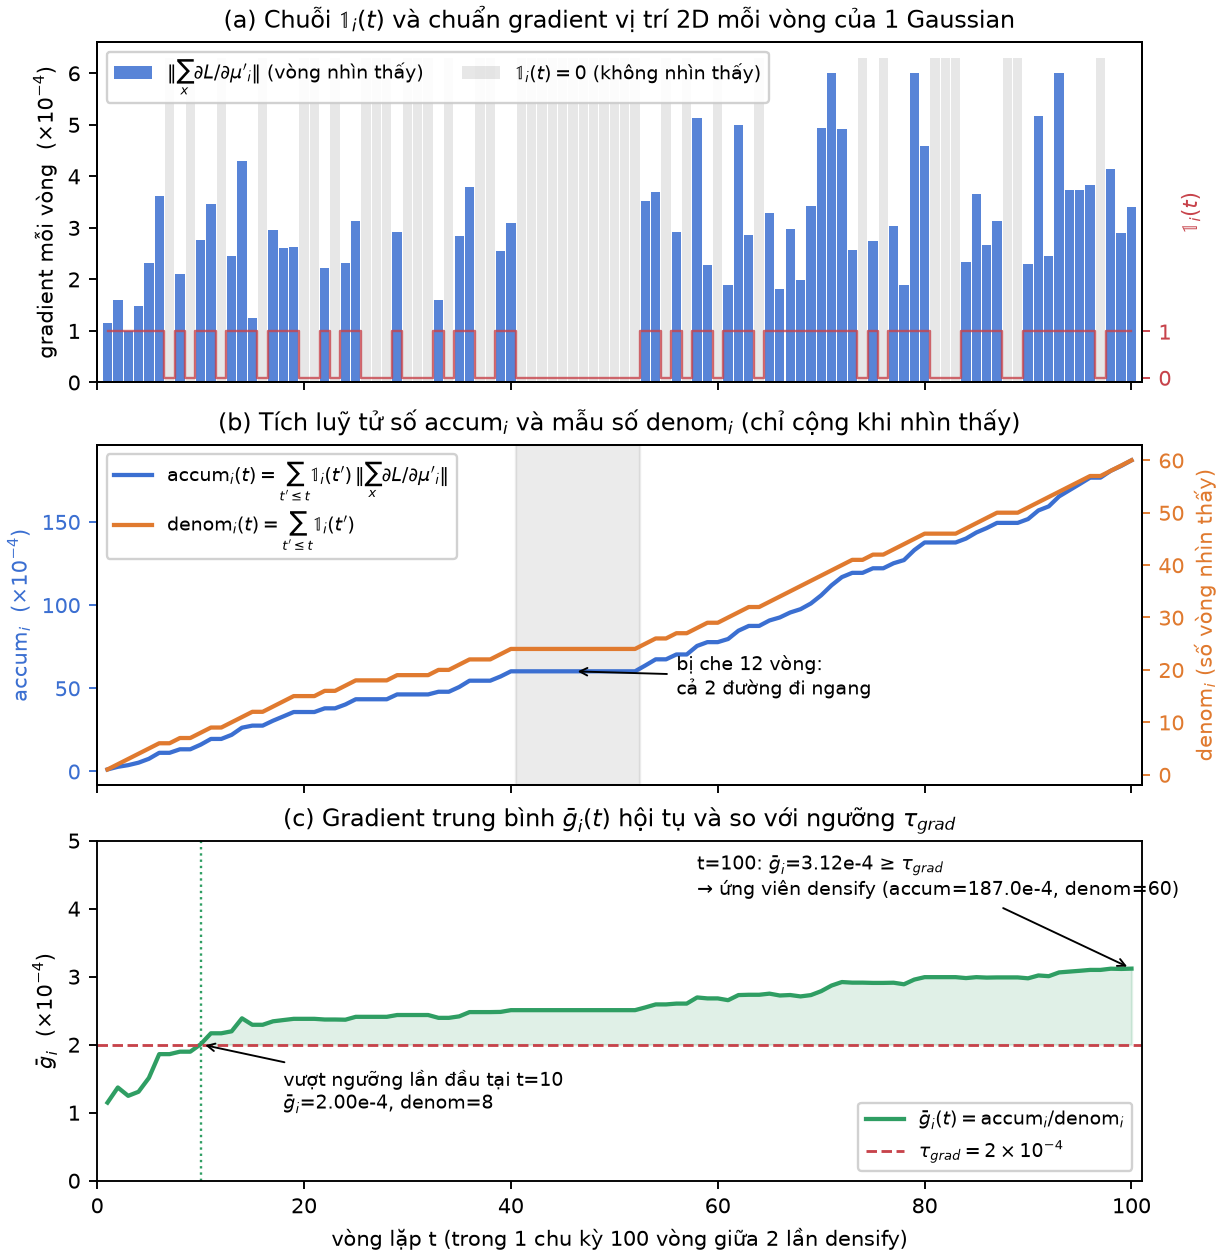
\includegraphics[width=0.36\linewidth]{fig_02_accum_denom.png}
\end{center}
\end{frame}

% --- Slide: Triệt tiêu gradient ---
\begin{frame}{Vấn đề "triệt tiêu gradient": xảy ra GIỮA CÁC PIXEL, không phải giữa các view}
\scriptsize
\textbf{Cách hiểu sai thường gặp:} "gradient từ các camera khác nhau kéo ngược chiều nhau nên triệt tiêu lẫn nhau".
Cách hiểu này \textbf{sai} với chính pipeline đã trình bày --- vì chuẩn $\lVert\cdot\rVert$ đã được lấy \textbf{trước
khi} cộng qua các view (slide trước), phép cộng \emph{giữa các view} không thể nào cho ra một tổng nhỏ hơn từng số hạng.
\begin{itemize}\itemsep1pt
    \item \textbf{Sự thật:} hiện tượng triệt tiêu thật sự xảy ra \emph{bên trong một lần render duy nhất}, \textbf{giữa
    các pixel} thuộc cùng footprint của \textbf{một} Gaussian. Ví dụ: nếu ảnh thật có một cạnh chạy ngang qua giữa
    Gaussian, nửa pixel bên trái có thể "kéo" $\mu'$ sang trái để khớp tốt hơn, nửa bên phải lại "kéo" sang phải ---
    khi \textbf{cộng vector gradient của từng pixel lại} (trước khi lấy chuẩn, ngay trong một lần render), hai lực kéo
    ngược chiều này có thể gần như \textbf{triệt tiêu nhau}, cho ra một vector tổng rất nhỏ dù bản thân mỗi pixel đều có
    gradient đáng kể.
    \item \textbf{Hệ quả nguy hiểm:} một Gaussian đang thực sự "dưới tái tạo" (thiếu chi tiết hình học ở đó) nhưng đối
    xứng theo một trục nào đó có thể bị đánh giá nhầm là "gradient thấp $\Rightarrow$ không cần densify" --- một điểm mù
    của cơ chế chỉ dùng gradient có dấu.
    \item \textbf{Cách khắc phục (kỹ thuật AbsGS):} renderer CUDA tính thêm, ngay trong backward pass, một kênh gradient
    \textbf{trị tuyệt đối theo từng pixel} \emph{trước khi} các dấu đối lập có cơ hội triệt tiêu nhau --- chính là kênh
    \texttt{xyz\_gradient\_accum\_abs} đã nhắc ở slide trước.
\end{itemize}
\begin{center}
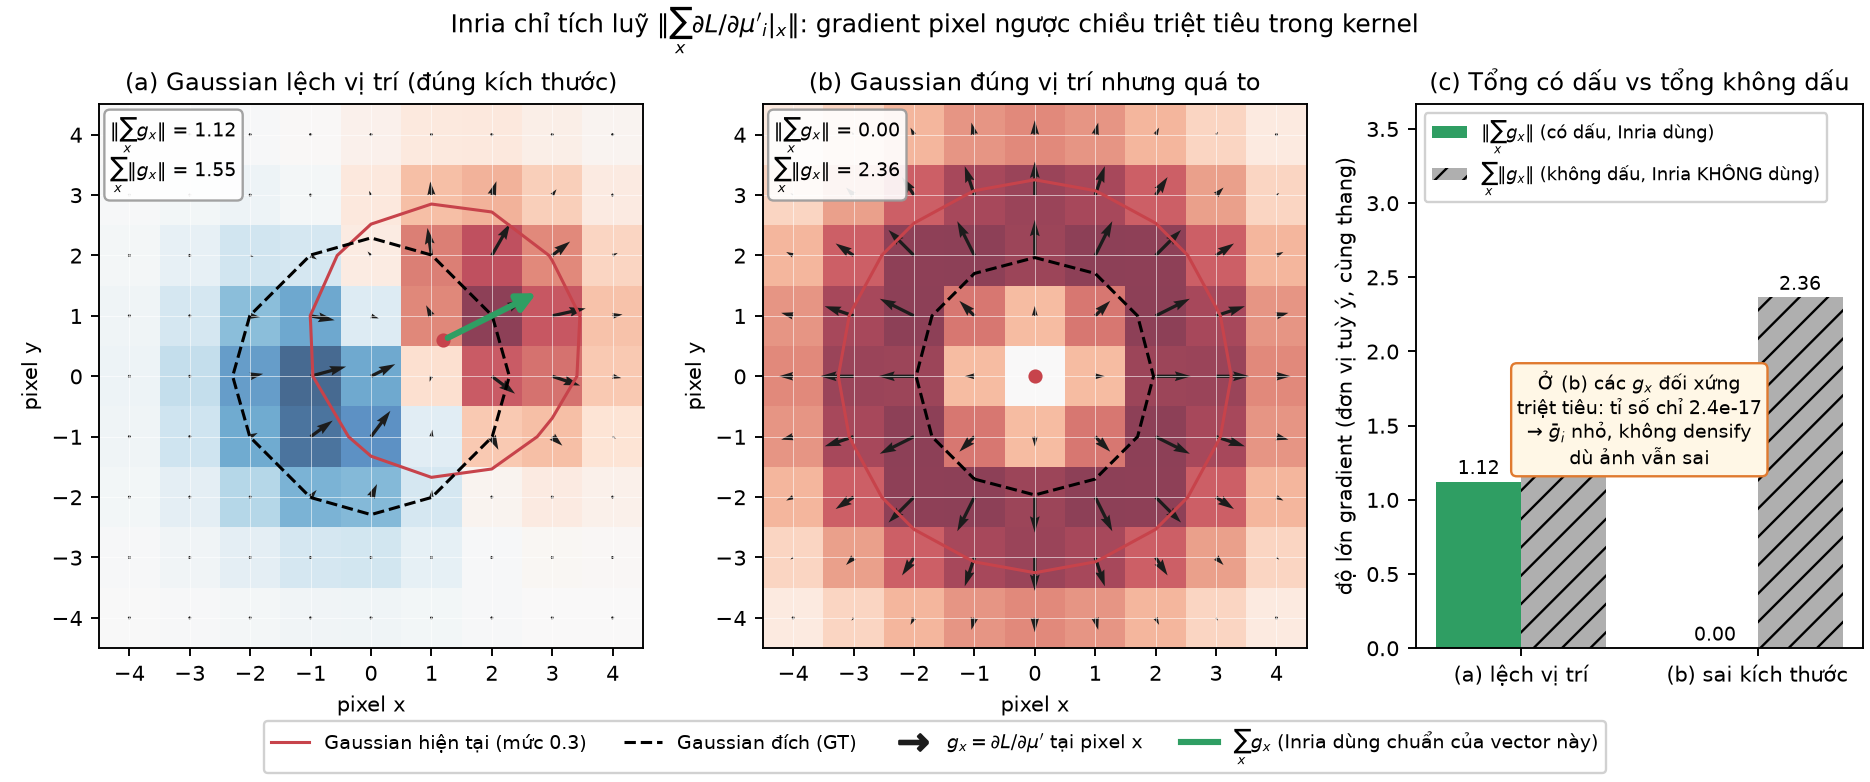
\includegraphics[width=0.36\linewidth]{fig_03_grad_cancel.png}
\end{center}
\end{frame}

% --- Slide: ADC tổng quan ---
\begin{frame}{Adaptive Density Control (ADC): khung chung}
\scriptsize
Có gradient tích luỹ $\bar g$ (và $\bar g_{\text{abs}}$) rồi, cứ mỗi \texttt{densification\_interval}$=100$ iteration
(bắt đầu từ \texttt{densify\_from\_iter}$=500$, tức lần đầu ở iteration $600$, tới \texttt{densify\_until\_iter}$=15\,000$),
3DGS thực hiện $3$ loại thao tác:
\begin{center}
\begin{tabular}{lll}
\toprule
\textbf{Thao tác} & \textbf{Điều kiện kích hoạt (ý tưởng)} & \textbf{Mục đích}\\
\midrule
\textbf{Clone} & gradient cao, Gaussian đang \emph{nhỏ} & bù \emph{under-reconstruction} (thiếu hình học)\\
\textbf{Split} & gradient cao, Gaussian đang \emph{to} & bù \emph{over-reconstruction} (Gaussian quá to, làm mờ chi tiết)\\
\textbf{Prune} & opacity quá thấp, hoặc quá to & dọn Gaussian không còn đóng góp\\
\bottomrule
\end{tabular}
\end{center}
"To/nhỏ" được so với ngưỡng \texttt{percent\_dense}$\times$\texttt{extent} (scene extent đã định nghĩa ở phần đầu):
Gaussian có trục dài nhất $\le$ ngưỡng này thì thuộc diện \textbf{clone}, lớn hơn thì thuộc diện \textbf{split}.
\begin{itemize}\itemsep1pt
    \item Trực giác: một Gaussian \textbf{nhỏ} nhưng vẫn còn gradient cao có nghĩa là "còn thiếu chi tiết ở đây, cần
    thêm quân số" $\to$ nhân bản. Một Gaussian \textbf{to} mà vẫn còn gradient cao nghĩa là "đang cố khớp một vùng có
    chi tiết mà một Gaussian không đủ" $\to$ chia nhỏ ra.
\end{itemize}
\end{frame}

% --- Slide: Clone ---
\begin{frame}{Clone: sao chép y nguyên, KHÔNG lệch vị trí}
\scriptsize
Khi một Gaussian nhỏ có gradient vượt ngưỡng, thao tác \texttt{densify\_and\_clone} thực hiện điều tưởng chừng đơn giản
đến bất ngờ: \textbf{sao chép y hệt} mọi tham số sang một Gaussian con mới --- \textbf{cùng vị trí}, cùng scale, cùng
rotation, cùng màu:
\[
\theta_{\text{con}} = \theta_{\text{cha}} \qquad (\text{không có bất kỳ }+\varepsilon\text{ hay lấy mẫu ngẫu nhiên nào})
\]
\begin{itemize}\itemsep1pt
    \item \textbf{Câu hỏi tự nhiên:} nếu hai bản sao giống hệt nhau, làm sao chúng tách ra để thực sự bổ sung chi tiết
    thay vì vẫn cứ trùng khít mãi? \textbf{Trả lời:} ngay sau khi sinh ra, hai Gaussian đi qua \textbf{optimizer độc
    lập} (mỗi Gaussian có trạng thái Adam --- \texttt{exp\_avg}, \texttt{exp\_avg\_sq} --- riêng của nó). Ở những bước
    gradient descent tiếp theo, dù xuất phát từ cùng một điểm, hai Gaussian này chịu nhiễu số học và các tương tác nhỏ
    khác nhau với các Gaussian lân cận $\Rightarrow$ dần dần bị "đẩy" ra hai hướng khác nhau một cách tự nhiên, giúp phủ
    tốt hơn vùng đang thiếu chi tiết.
    \item Các bộ đếm thống kê (\texttt{xyz\_gradient\_accum}, \texttt{denom}, v.v.) của bản sao mới được \textbf{reset về
    $0$} ngay sau khi sinh --- lịch sử theo dõi của nó hoàn toàn tách biệt với Gaussian cha kể từ thời điểm này.
\end{itemize}
\begin{center}
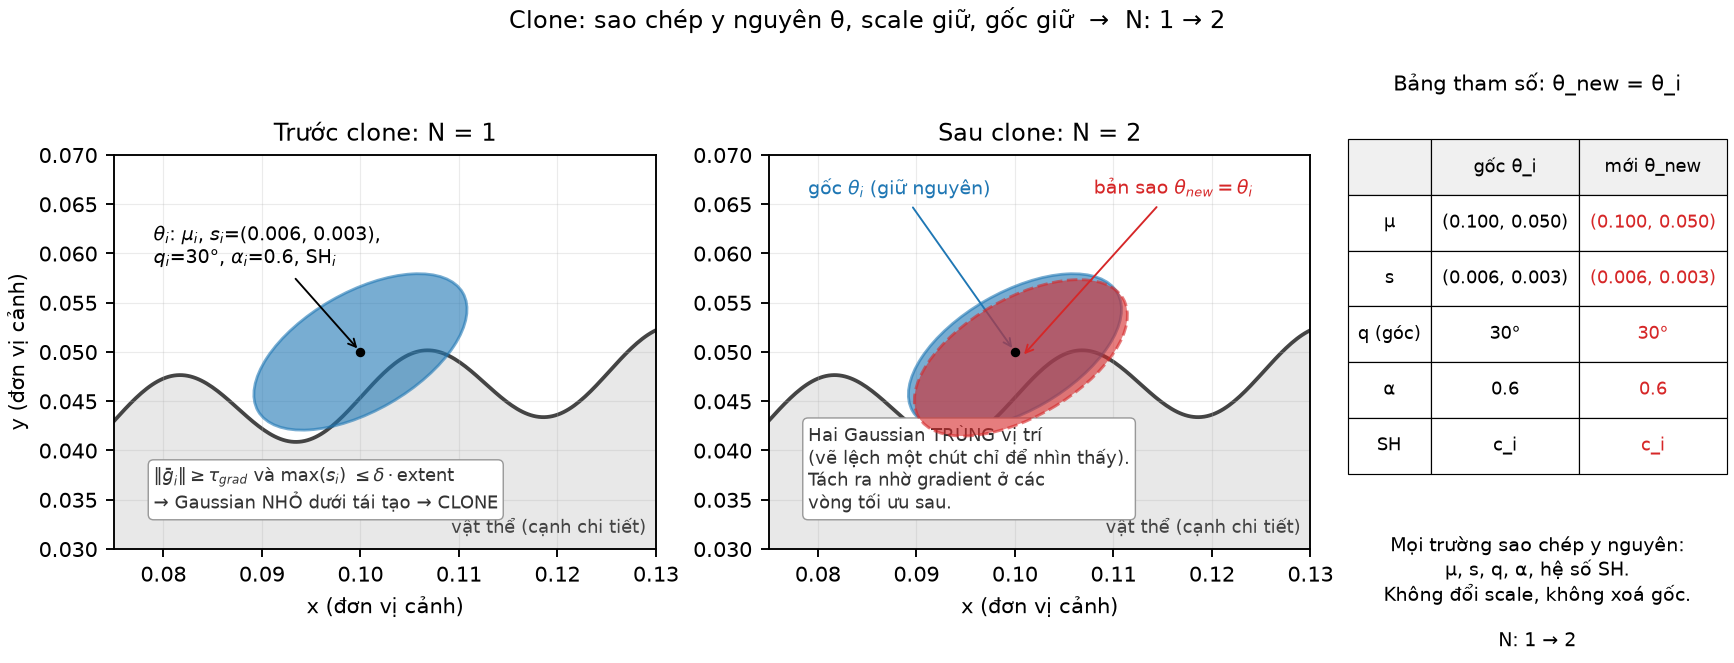
\includegraphics[width=0.30\linewidth]{fig_08_clone_before_after.png}
\end{center}
\end{frame}
   % Slide 13-16 Gradient biên, Tổng kết training loop, ADC tổng quan, Tích luỹ gradient

\section{Adaptive Density Control}
% ===== FILE 5/9: Split nguyên bản, Sigmoid nghịch đảo, Quỹ đạo opacity reset, Histogram reset, Tổng kết pipeline gốc =====

% --- Slide: Split (3DGS nguyên bản) ---
\begin{frame}{Split nguyên bản: lấy mẫu ngẫu nhiên quanh Gaussian cha}
\scriptsize
Khi một Gaussian \textbf{to} (trục dài nhất $>$ ngưỡng \texttt{percent\_dense}$\times$extent) vẫn còn gradient trị
tuyệt đối cao, cơ chế \textbf{split nguyên bản} (\texttt{densify\_and\_split}, \texttt{gaussian\_model.py:866--889})
sinh ra $N=2$ Gaussian con để "chia việc" khớp chi tiết:
\[
x_{\text{con}} = \mu_{\text{cha}} + R(q)\,\varepsilon,\qquad \varepsilon\sim\mathcal{N}(0,\mathrm{diag}(s_{\text{cha}})^2),
\qquad s_{\text{con}} = \frac{s_{\text{cha}}}{0.8\,N} = \frac{s_{\text{cha}}}{1.6}
\]
\begin{itemize}\itemsep1pt
    \item Vị trí mỗi con được \textbf{lấy mẫu ngẫu nhiên} từ một phân phối Gaussian có độ lệch chuẩn chính bằng scale
    của cha, sau đó xoay theo hướng $R(q)$ của cha --- tức là các con rải rác quanh cha, theo đúng hình dạng ellipsoid
    của cha (không rải đều hình cầu).
    \item Cả $N=2$ con đều bị chia scale cho \textbf{cùng một hệ số $1.6$ trên cả 3 trục}, bất kể trục nào mới thực sự
    là trục "quá to" gây ra vấn đề --- đây là điểm mà cơ chế split dị hướng của SADGS (phần sau bài giảng) cải tiến.
    \item Gaussian cha bị xoá ngay sau khi sinh $2$ con --- tổng số Gaussian tăng thêm đúng $1$ đơn vị mỗi lần một điểm
    bị split.
\end{itemize}
\begin{center}
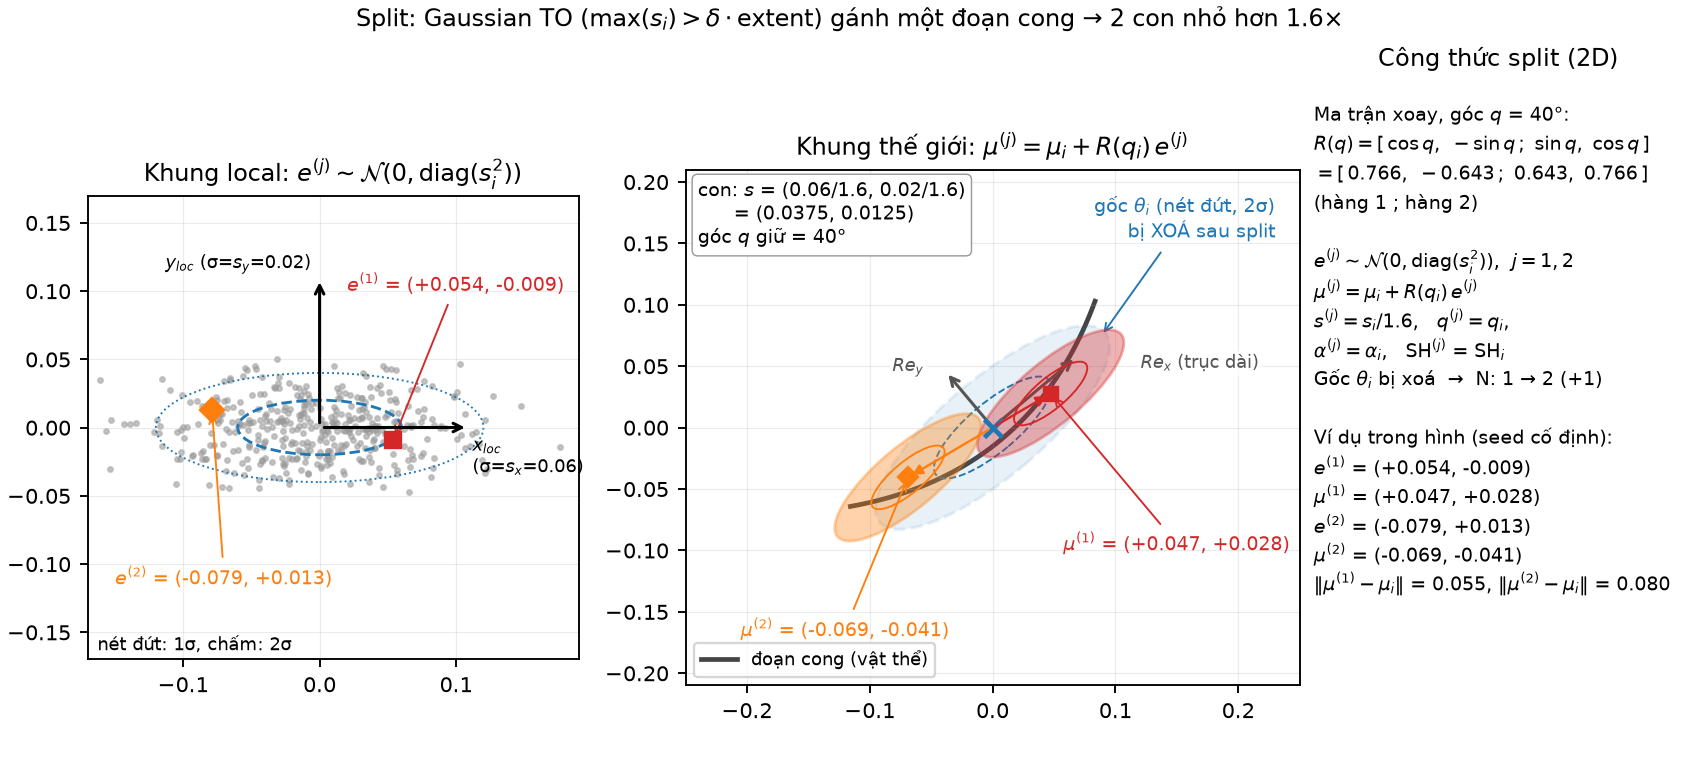
\includegraphics[width=0.4\linewidth]{fig_09_split_geometry.png}
\end{center}
\end{frame}

% --- Slide: Sigmoid nghịch đảo & opacity reset ---
\begin{frame}{Vì sao lưu opacity dưới dạng logit? Và cơ chế reset định kỳ}
\scriptsize
Opacity $\alpha\in(0,1)$ được lưu nội bộ dưới dạng \textbf{logit} $o=\sigma^{-1}(\alpha)=\ln\!\frac{\alpha}{1-\alpha}$
(giá trị thực bất kỳ), rồi đi qua sigmoid $\alpha=\sigma(o)$ khi cần dùng --- giống hệt lý do dùng $\exp$ cho scale: để
mọi số thực đều tương ứng với một giá trị $\alpha$ \textbf{hợp lệ}, không cần ràng buộc \texttt{clamp} thủ công trong
quá trình tối ưu bằng gradient descent.
\begin{itemize}\itemsep1pt
    \item \textbf{Vì sao cần reset opacity định kỳ?} Nếu để tự nhiên, nhiều Gaussian "chết dần" (opacity giảm về rất
    thấp) vẫn tồn tại lâu, chiếm bộ nhớ mà không đóng góp gì đáng kể. Mỗi \texttt{opacity\_reset\_interval}$=3000$
    iteration (\emph{với điều kiện} $\texttt{iteration}<\texttt{densify\_until\_iter}=15\,000$, tức \textbf{chỉ đúng
    $4$ lần}: tại $3\text{k},6\text{k},9\text{k},12\text{k}$), toàn bộ opacity bị \textbf{giảm mạnh}:
    \[
    \alpha \leftarrow \alpha_{\text{cũ}} \times \texttt{opacity\_reset\_decay} = \alpha_{\text{cũ}}\times 0.1
    \]
    \item \textbf{Cơ chế "sàng lọc":} Gaussian nào thực sự hữu ích (đang đóng góp giảm loss) sẽ nhanh chóng \textbf{hồi
    phục} opacity qua vài trăm bước gradient tiếp theo; Gaussian nào không còn đóng góp thì opacity vẫn ở mức thấp và
    sẽ bị prune ở đợt dọn dẹp kế tiếp (slide sau).
    \item Vì reset \textbf{dừng hẳn} sau iteration $15\,000$, nửa sau của quá trình train không còn cơ chế chủ động nào
    "sàng lọc lại" opacity định kỳ nữa.
\end{itemize}
\begin{center}
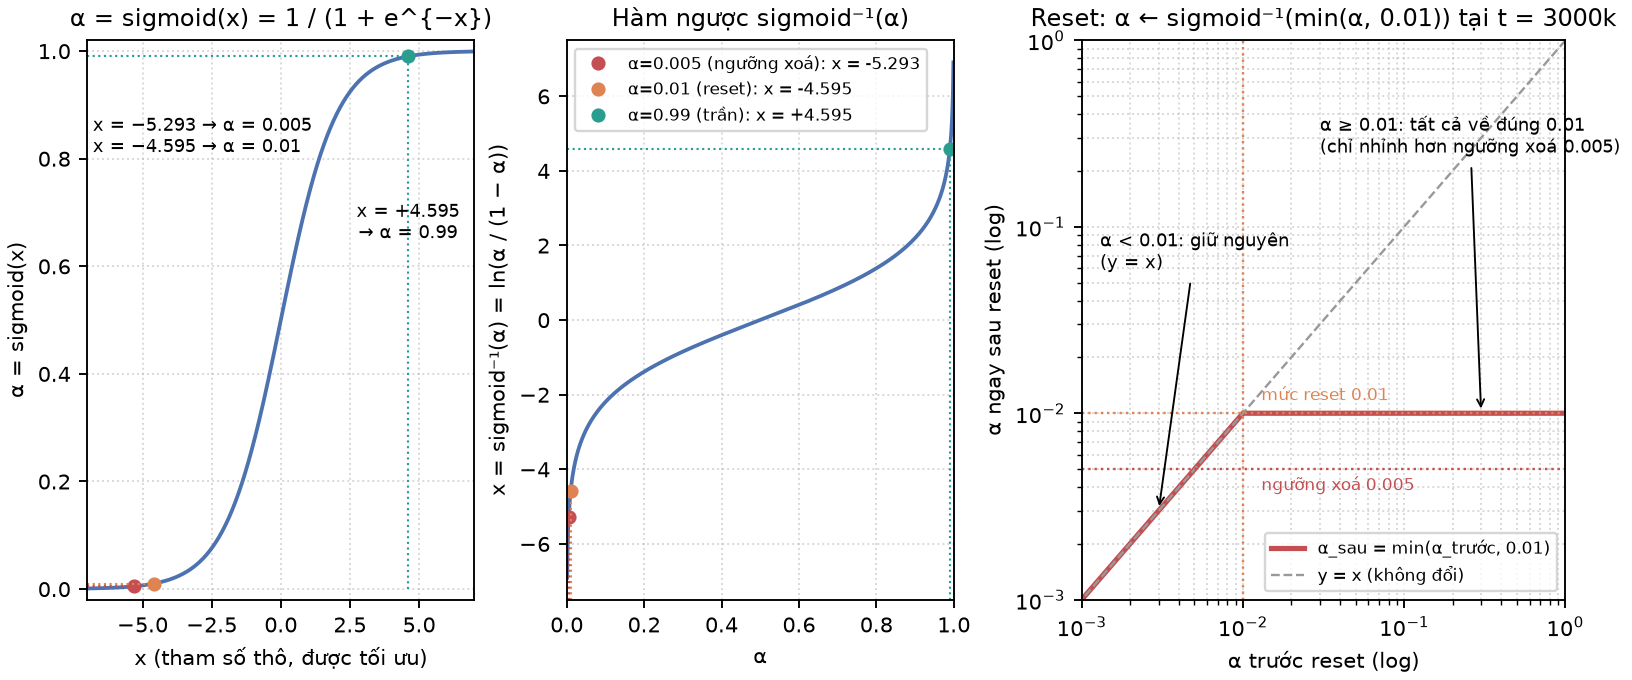
\includegraphics[width=0.30\linewidth]{fig_16_sigmoid_inverse.png}
\end{center}
\end{frame}

% --- Slide: Quỹ đạo opacity qua các lần reset ---
\begin{frame}{Quan sát quỹ đạo opacity của một Gaussian qua nhiều lần reset}
\scriptsize
Theo dõi $\alpha(t)$ của một Gaussian cụ thể xuyên suốt quá trình train cho thấy rõ "nhịp điệu" của cơ chế reset: mỗi
lần chạm mốc reset ($3\text{k},6\text{k},9\text{k},12\text{k}$), $\alpha$ bị "đập" xuống còn $10\%$ giá trị trước đó,
sau đó \textbf{leo dần trở lại} nếu Adam vẫn còn nhận được gradient khuyến khích tăng opacity tại vị trí đó.
\begin{itemize}\itemsep1pt
    \item Một Gaussian \textbf{quan trọng} (đang giúp giảm loss thật sự): sau mỗi lần reset, $\alpha$ hồi phục nhanh,
    thường vượt lại mức trước khi reset trong vòng vài trăm iteration.
    \item Một Gaussian \textbf{dư thừa} (không còn đóng góp rõ rệt, ví dụ đã bị Gaussian khác lân cận "lấn sân"): sau
    reset, $\alpha$ hồi phục rất chậm hoặc gần như không hồi phục --- nó sẽ nằm dưới ngưỡng prune ở lần dọn tiếp theo.
    \item Cơ chế này về bản chất là một dạng \textbf{"kiểm tra sức khỏe" định kỳ} cho toàn bộ quần thể Gaussian, tách
    biệt hẳn với cơ chế clone/split/prune dựa trên gradient/kích thước đã nói ở các slide trước.
\end{itemize}
\begin{center}
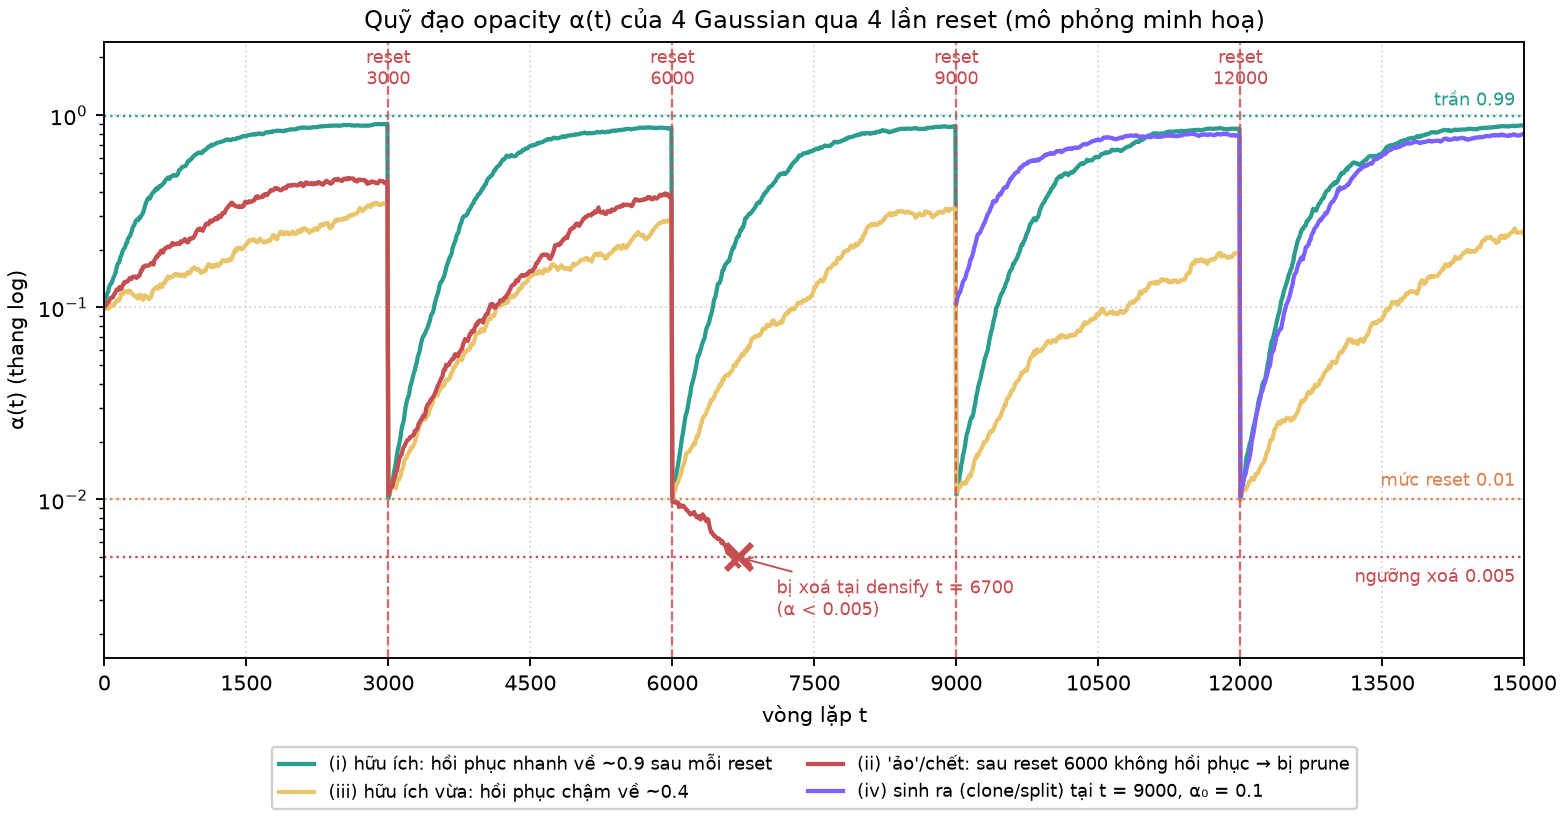
\includegraphics[width=0.36\linewidth]{fig_17_opacity_trajectory.png}
\end{center}
\end{frame}

% --- Slide: Histogram trước/sau reset ---
\begin{frame}{Nhìn trên toàn bộ quần thể: phân bố opacity trước và sau reset}
\scriptsize
Thay vì theo dõi một Gaussian, hãy nhìn \textbf{toàn bộ phân bố} opacity của mọi Gaussian ngay trước và ngay sau một
lần reset. Ngay sau reset, toàn bộ phân bố bị "nén" mạnh về phía các giá trị thấp (do nhân với $0.1$) --- gần như mọi
Gaussian đều tạm thời "mờ đi" đồng loạt.
\begin{itemize}\itemsep1pt
    \item Điều thú vị xảy ra ở các iteration \textbf{sau} reset: phân bố dần \textbf{tách thành hai nhóm} --- một nhóm
    hồi phục nhanh trở lại vùng opacity cao (Gaussian hữu ích), một nhóm tiếp tục nằm lại vùng thấp (ứng viên prune).
    \item Đây chính là hiệu ứng "sàng lọc" đã mô tả ở hai slide trước, nhưng nhìn dưới góc độ \textbf{thống kê quần
    thể} thay vì một cá thể --- một cách trực quan để kiểm chứng cơ chế reset có thực sự đang "phân loại" Gaussian hữu
    ích/dư thừa hay không trong một lần chạy huấn luyện cụ thể.
\end{itemize}
\begin{center}
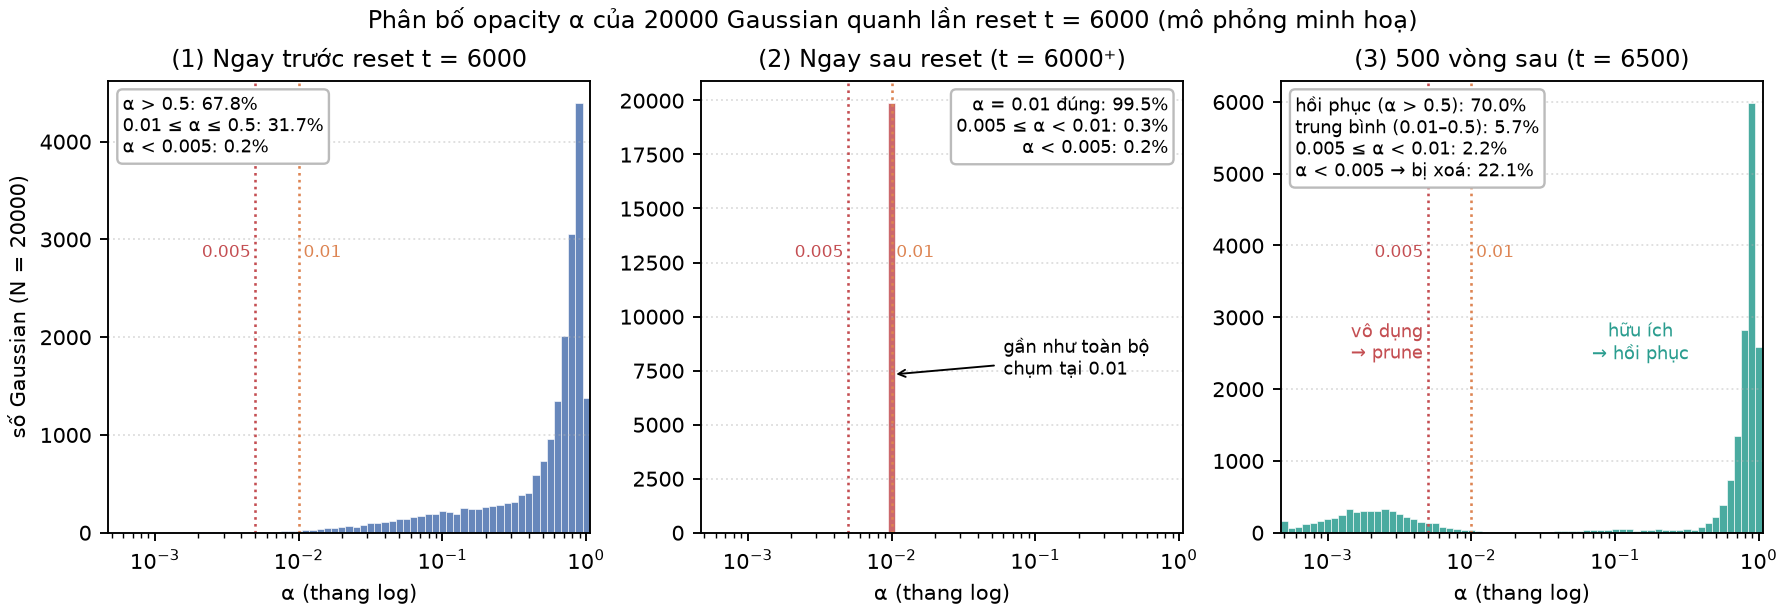
\includegraphics[width=0.36\linewidth]{fig_18_hist_reset.png}
\end{center}
\end{frame}

% --- Slide: Tổng kết pipeline 3DGS gốc ---
\begin{frame}{Tổng kết: pipeline 3DGS gốc, đầu-cuối}
\scriptsize
Gộp lại toàn bộ phần vừa trình bày thành một vòng lặp duy nhất:
\[
\text{SfM/COLMAP} \to \{\mu,\Sigma,\alpha,c\}_{i=1}^N \xrightarrow{\text{EWA}} \text{ellipse 2D}
\xrightarrow{\text{compact box}} \text{tile} \xrightarrow{\text{blend}} C(x)
\xrightarrow{\mathcal{L}} \nabla\theta \xrightarrow{\text{Adam}} \theta_{\text{mới}}
\]
lặp lại hàng chục nghìn lần, với riêng mỗi $100$ iteration lại chen thêm bước \textbf{ADC} (clone/split/prune) dựa trên
gradient tích luỹ, và mỗi $3000$ iteration (tới $15\,000$) lại reset opacity một lần.
\begin{itemize}\itemsep1pt
    \item \textbf{Điểm mạnh của thiết kế này:} hoàn toàn tường minh và khả vi từ đầu đến cuối --- không hộp đen, mọi
    bước đều có thể kiểm tra, gỡ lỗi; render thời gian thực ngay sau khi train xong.
    \item \textbf{Điểm còn hạn chế, là động lực cho phần tiếp theo của bài giảng:} tín hiệu densify \textbf{chỉ dựa vào
    gradient} --- một đại lượng phản ánh \emph{trạng thái hội tụ hiện tại} của loss, chứ không trực tiếp đo "ảnh này còn
    thiếu bao nhiêu \% chi tiết tần số cao chưa được biểu diễn, theo tỉ lệ nào". Hai Gaussian có cùng độ lớn gradient có
    thể đang thiếu hụt hình học ở hai \emph{quy mô} rất khác nhau (một cái thiếu chi tiết rất mịn, một cái thiếu cấu
    trúc thô hơn nhiều) --- gradient một mình không phân biệt được điều này.
\end{itemize}
\begin{center}
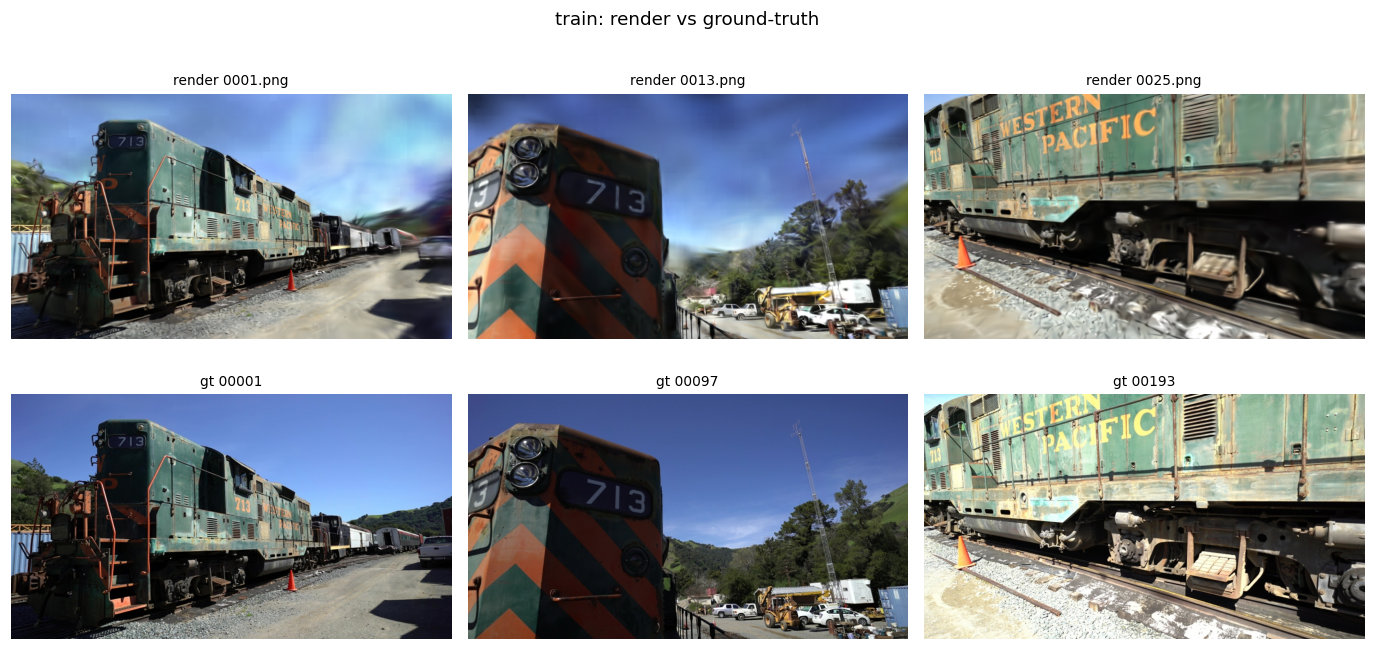
\includegraphics[width=0.34\linewidth]{samples_train.png}\\
\captionof{figure}{\footnotesize Ảnh render minh hoạ (định tính, không kèm số đo benchmark).}
\end{center}
\end{frame}
   % Slide 17-20 Gradient cancellation, Clone, Split, Prune multi-view
% ===== FILE 6/9: Động lực SADGS, Kim tự tháp đa tỉ lệ, Structure tensor gộp, Trị riêng & bước sóng, Chiếu trục Gaussian =====

% --- Slide: Động lực SADGS ---
\begin{frame}{SADGS: bổ sung tín hiệu tần số cho Adaptive Density Control}
\scriptsize
Nhắc lại hạn chế đã nêu ở cuối phần trước: gradient một mình không đo được "Gaussian này đang to/nhỏ \textbf{so với chi
tiết ảnh cần biểu diễn} theo tỉ lệ nào". \textbf{Ý tưởng cốt lõi của SADGS} (Structure-Aware Densification): đo trực
tiếp một tỉ số hình học giữa \textbf{kích thước Gaussian sau khi chiếu lên màn hình} và \textbf{kích thước chi tiết ảnh
cục bộ} (một dạng "bước sóng" texture) tại đúng vị trí Gaussian đó --- gọi tỉ số này là $\eta$.
\begin{itemize}\itemsep2pt
    \item Nếu Gaussian \textbf{to hơn} chi tiết cần biểu diễn ($\eta>1$): nó đang "nuốt chửng", làm mờ mất chi tiết đó
    --- cần \textbf{split} thành các mảnh nhỏ hơn, và quan trọng hơn: chia \textbf{đúng theo trục} bị vi phạm, không
    phải chia đều mọi trục như cơ chế gốc.
    \item Nếu Gaussian \textbf{nhỏ hơn nhiều} so với chi tiết cục bộ ($\eta\le0.1$): nó đang "phục vụ thừa" một vùng gần
    như không đổi --- một Gaussian lớn hơn cũng đủ sức biểu diễn vùng đó --- là ứng viên \textbf{prune}.
    \item \textbf{Điểm quan trọng cần nhấn mạnh:} SADGS \textbf{không thay thế} khung ADC gốc vừa học --- nó \textbf{kế
    thừa toàn bộ} khung clone/split/prune, chỉ \textbf{bổ sung thêm} một điều kiện kích hoạt dựa trên $\eta$, kết hợp
    bằng phép \texttt{OR} với điều kiện gradient cũ (chi tiết đầy đủ ở phần sau).
    \item Bốn slide tiếp theo xây dựng $\eta$ từ con số $0$: ảnh gốc $\to$ kim tự tháp đa tỉ lệ $\to$ structure tensor
    $\to$ trị riêng $\to$ bước sóng cục bộ $\to$ chiếu trục Gaussian lên màn hình $\to$ $\eta$.
\end{itemize}
\end{frame}

% --- Slide: Kim tự tháp đa tỉ lệ ---
\begin{frame}{Bước 1: kim tự tháp đa tỉ lệ (multiscale) trên ảnh GT}
\scriptsize
Trước khi có thể so sánh "kích thước Gaussian" với "kích thước chi tiết ảnh", cần một cách đo \textbf{chi tiết ảnh có
kích thước bao nhiêu} tại mỗi vị trí. Hàm \texttt{get\_multiscale\_structure\_tensor\_v1}
(\texttt{utils/loss\_utils.py:232--}) làm mờ dần ảnh gốc qua nhiều tầng $i=0,\dots,\texttt{levels}-1$ (mặc định $3$
tầng), tầng sau mờ hơn tầng trước theo một tỉ lệ cố định:
\[
\sigma_i=\sigma_0\cdot(\texttt{octave\_step})^i,\quad \texttt{octave\_step}=1.5,\qquad
b_i = \big\lVert I^{(i-1)}_{\text{mờ}} - I^{(i)}_{\text{mờ}}\big\rVert_2 \ \ (\text{DoG, xấp xỉ Laplacian})
\]
\begin{itemize}\itemsep1pt
    \item $b_i$ (\emph{Difference-of-Gaussians}, kỹ thuật kinh điển trong thị giác máy tính, ví dụ dùng trong SIFT): là
    \textbf{bản đồ năng lượng cạnh} tại tầng $i$ --- vùng phẳng cho $b_i\approx0$, vùng có cạnh/chi tiết rõ cho $b_i$ lớn.
    \item Tần số ứng với mỗi tầng: $f_i=1/(\texttt{octave\_step})^i$ --- tầng $i$ càng lớn (mờ càng nhiều) thì $f_i$
    càng nhỏ, ứng với chi tiết \textbf{thô} hơn.
    \item \textbf{Vì sao cần nhiều tỉ lệ chứ không chỉ một?} Một hoạ tiết lặp (ví dụ vân gỗ, gạch lát) có thể "rõ" khi
    nhìn ở độ phân giải mịn nhưng gần như "biến mất" khi nhìn ở độ phân giải thô, hoặc ngược lại với cấu trúc lớn (viền
    một toà nhà). Gộp nhiều tầng tránh bỏ sót chi tiết chỉ tồn tại rõ ràng ở một quy mô riêng.
\end{itemize}
\begin{center}
\includegraphics[width=0.4\linewidth]{01_pyramid_levels.png}
\end{center}
\end{frame}

% --- Slide: Structure tensor gộp đa tỉ lệ ---
\begin{frame}{Bước 2: gộp thành một structure tensor duy nhất $\hat J$}
\scriptsize
Tại mỗi tầng $i$, ta có thể tính một \textbf{structure tensor} $J_i=\begin{psmallmatrix}S_{xx}&S_{xy}\\S_{xy}&S_{yy}\end{psmallmatrix}_i$
--- một ma trận $2\times2$ cổ điển trong xử lý ảnh, đo \textbf{hướng} và \textbf{cường độ} biến thiên cục bộ (dựng từ
tích ngoài của vector gradient ảnh, làm mờ nhẹ để ổn định). Structure tensor gộp toàn bộ các tầng theo trọng số
(\texttt{loss\_utils.py:283--300}):
\[
\boxed{\;\hat J = \frac{\sum_i \big(J_i/\mathrm{tr}J_i\big)\,w_i\,f_i^2}{\sum_i w_i}\;},\qquad w_i = b_i^{\,p}\ (p=3\text{, mặc định})
\]
\begin{itemize}\itemsep1pt
    \item $J_i/\mathrm{tr}J_i$: \textbf{chuẩn hoá theo vết} --- mỗi tầng chỉ còn đóng góp thông tin \emph{hướng/hình
    dạng} (dị hướng của biến thiên), loại bỏ ảnh hưởng của việc tầng nào đó có năng lượng tuyệt đối lớn hơn tầng khác một cách tình cờ.
    \item $w_i=b_i^3$: tầng nào có cạnh/chi tiết rõ ràng hơn ($b_i$ lớn hơn) được \textbf{"tin cậy" nhiều hơn} khi gộp;
    luỹ thừa $3$ khuếch đại sự chênh lệch này khá mạnh, để tầng "nhiễu" (ít cấu trúc) không làm loãng thông tin từ tầng
    có cấu trúc rõ.
    \item $f_i^2$: hệ số quy đổi để các tầng --- vốn bị làm mờ ở các $\sigma_i$ khác nhau --- được đưa về \textbf{cùng
    một thang tần số vật lý} trước khi cộng gộp.
    \item Kết quả $\hat J=(S_{xx},S_{xy},S_{yy})$ chính là "nguyên liệu" dùng lại xuyên suốt các bước tính $\eta$ tiếp theo.
\end{itemize}
\begin{center}
\includegraphics[width=0.4\linewidth]{01_structure_tensor_channels.png}
\end{center}
\end{frame}

% --- Slide: Trị riêng & bước sóng cục bộ ---
\begin{frame}{Bước 3: trị riêng của $\hat J$ $\to$ bước sóng cục bộ $w_{\min}$}
\scriptsize
Từ ma trận $\hat J$, trích ra \textbf{trị riêng lớn nhất} $\lambda_1$ (\texttt{utils/freq\_utils.py:313--334}) --- đại
lượng vô hướng duy nhất cần cho bước tiếp theo:
\[
\lambda_1=\frac{\mathrm{tr}\hat J}{2}+\sqrt{\Big(\frac{\mathrm{tr}\hat J}{2}\Big)^2-\det\hat J},\qquad
\boxed{\;w_{\min}=\dfrac{1}{\sqrt{\lambda_1}+10^{-5}}\;}
\]
\begin{itemize}\itemsep1pt
    \item $\lambda_1$ tỉ lệ với \textbf{năng lượng gradient bình phương} theo hướng biến thiên mạnh nhất tại điểm đó ---
    vùng có cạnh sắc, chi tiết dày đặc sẽ cho $\lambda_1$ lớn; vùng phẳng cho $\lambda_1\approx0$.
    \item Phép biến đổi "năng lượng $\to$ bước sóng" dùng nghịch đảo căn bậc hai: trực giác là năng lượng gradient cao
    tương ứng với \textbf{tần số không gian cao} (chi tiết mịn, đổi nhanh theo pixel), mà tần số cao nghĩa là \textbf{bước
    sóng ngắn} --- do đó $\lambda_1$ lớn $\Rightarrow$ $w_{\min}$ \textbf{nhỏ}. Ngược lại, vùng phẳng $\lambda_1\to0$ cho
    $w_{\min}\to10^5$ (rất lớn --- "không có chi tiết nào cần bám theo ở đây cả").
    \item $w_{\min}$ sẽ đóng vai trò \textbf{mẫu số}, là "cây thước" để so sánh với kích thước Gaussian ở bước tính $\eta$ ngay sau đây.
\end{itemize}
\begin{center}
\includegraphics[width=0.4\linewidth]{02_wavelength_eigen.png}
\end{center}
\end{frame}

% --- Slide: Chiếu trục Gaussian lên màn hình ---
\begin{frame}{Bước 4: chiếu 3 trục chính của Gaussian lên màn hình}
\scriptsize
Có "cây thước" $w_{\min}$ rồi, giờ cần đo "kích thước Gaussian" theo đúng đơn vị tương thích (pixel trên màn hình).
Hàm \texttt{compute\_projected\_axes\_subset} (\texttt{utils/freq\_utils.py:116--178}) dùng lại đúng Jacobian $J$ của
phép chiếu pinhole đã học ở phần đầu bài giảng:
\[
\boxed{\;a_j = J\,(R_{\text{view}}R_i)\,\mathrm{diag}(s)\,e_j\;},\qquad \ell_j = \lVert a_j\rVert = \sqrt{u_j^2+v_j^2+10^{-8}}
\]
\begin{itemize}\itemsep1pt
    \item $R_i\,\mathrm{diag}(s)\,e_j$: véc-tơ trục chính thứ $j$ của ellipsoid ($j=1,2,3$, ba trục vuông góc của
    ellipsoid trong không gian world), có độ dài $=s_j$.
    \item $R_{\text{view}}$ xoay véc-tơ đó sang hệ toạ độ camera; $J$ tuyến tính hoá phép chiếu phối cảnh, đánh giá tại
    đúng vị trí $\mu$ của Gaussian --- giống hệt cách dùng $J$ trong EWA splatting ở phần render.
    \item $\ell_j$ là \textbf{độ dài tính bằng pixel}, sau khi chiếu, của trục chính thứ $j$ --- đây chính là tử số
    của $\eta$.
    \item Mỗi Gaussian có \textbf{3 giá trị} $\ell_1,\ell_2,\ell_3$ (ứng với 3 trục chính hình học, \textbf{không phải}
    3 kênh màu R/G/B) --- nhờ đó SADGS biết được Gaussian đang vi phạm \emph{theo hướng cụ thể nào}, để sau này split
    \emph{đúng trục} đó thay vì chia đều mọi hướng.
\end{itemize}
\begin{center}
\includegraphics[width=0.4\linewidth]{02_jacobian_axes.png}
\end{center}
\end{frame}
   % Reset opacity, Sơ đồ quyết định densify
% ===== FILE 7/9: Eta (Nyquist), Ngưỡng & đa view, Split dị hướng (lưới), Split dị hướng (bậc thang k), Prune đa view =====

% --- Slide: Tỉ số eta — trực giác Nyquist ---
\begin{frame}{Bước 5: $\eta=\ell/w_{\min}$ --- trực giác Nyquist}
\scriptsize
Giờ đã có cả tử số ($\ell$, kích thước Gaussian đã chiếu) lẫn mẫu số ($w_{\min}$, bước sóng chi tiết cục bộ), định nghĩa
tỉ số cấu trúc:
\[
\boxed{\;\eta_j=\dfrac{\ell_j}{w_{\min}}\;}\qquad(\texttt{eta\_compute\_mode="wavelength"}\text{, mặc định}, \texttt{freq\_utils.py:348})
\]
Đây là một ngưỡng \textbf{hình học thuần tuý} (so sánh hai độ dài), \textbf{không phải} một mô hình vật lý về suy hao
biên độ tín hiệu --- tên gọi "trực giác Nyquist" chỉ mượn ý tưởng chung của lý thuyết lấy mẫu: muốn biểu diễn đúng một
dao động, "đơn vị lấy mẫu" (ở đây là Gaussian) phải đủ nhỏ so với chu kỳ của dao động đó.
\begin{itemize}\itemsep1pt
    \item $\eta>1$: $\ell$ \textbf{rộng hơn cả một chu kỳ} chi tiết $\Rightarrow$ một Gaussian không đủ khả năng bám
    theo dao động đó $\Rightarrow$ ứng viên \textbf{SPLIT}.
    \item $0.1<\eta\le1$: kích thước tương xứng với chi tiết cần biểu diễn $\Rightarrow$ \textbf{GIỮ NGUYÊN}.
    \item $\eta\le0.1$: $\ell$ nhỏ hơn $w_{\min}$ tới hơn $10$ lần --- Gaussian đang "phủ thừa" một vùng gần như không
    đổi $\Rightarrow$ ứng viên \textbf{PRUNE}.
    \item \textbf{Lưu ý về tài liệu nội bộ code:} một số dòng docstring (\texttt{gaussian\_model.py:837--840}) mô tả
    $\eta\sim(\sigma\omega)^2$ (quan hệ \emph{bậc hai}) --- nhưng công thức \textbf{thực sự được tính và dùng} ở trên là
    quan hệ \textbf{tuyến tính} theo kích thước. Toàn bộ bài giảng này bám theo công thức \emph{thực chạy}, không theo
    docstring (vốn có thể là tài liệu chưa cập nhật theo code).
\end{itemize}
\begin{center}
\includegraphics[width=0.62\linewidth]{02_nyquist.png}
\end{center}
\end{frame}

% --- Slide: Ngưỡng phân loại & tích luỹ đa view ---
\begin{frame}{Bước 6: ngưỡng phân loại và tích luỹ NHẤT QUÁN ĐA VIEW}
\scriptsize
Ngưỡng cố định trong code: \texttt{TAU\_HIGH=1.0}, \texttt{TAU\_LOW=0.1} (\texttt{freq\_utils.py:395--396}). Mỗi lần
render một view, lấy $\eta_{\max}=\max_j\eta_j$ (giá trị lớn nhất trong 3 trục) và cộng $1$ vào đúng một trong ba bộ đếm:
\[
\texttt{eta\_high\_count} \;(\eta_{\max}>1)\qquad
\texttt{eta\_mid\_count}\qquad
\texttt{eta\_low\_count}\;(\eta_{\max}\le0.1)
\]
Tới kỳ densify (mỗi $100$ iteration), các bộ đếm này được quy ra \textbf{tỉ lệ nhất quán qua nhiều view}
(\texttt{train.py:341--353}) --- đây chính là điểm khác biệt lớn nhất về \emph{triết lý} so với 3DGS gốc, vốn chỉ nhìn
vào gradient tích luỹ tại \textbf{một} thời điểm cuối cùng để quyết định, không phân biệt rõ ràng "có bao nhiêu góc
nhìn đồng ý với nhau":
\[
\text{high\_ratio}=\frac{\texttt{eta\_high\_count}}{\texttt{accum\_view\_count}}>0.8\qquad
\text{low\_ratio}=\frac{\texttt{eta\_low\_count}}{\texttt{accum\_view\_count}}>0.8
\]
\begin{itemize}\itemsep1pt
    \item \textbf{Trực giác:} chỉ khi \textbf{đa số áp đảo} ($>80\%$) các góc nhìn quan sát được đều đồng thuận rằng
    Gaussian "quá to" (hoặc "quá nhỏ"), quyết định split/prune mới được kích hoạt --- giúp tránh phản ứng thái quá theo
    nhiễu của một góc chụp bất thường (ví dụ do occlusion, ánh sáng loá, hay góc nhìn gần như cạnh của ellipsoid).
\end{itemize}
\begin{center}
\includegraphics[width=0.4\linewidth]{03_timeline_reset.png}
\end{center}
\end{frame}

% --- Slide: Split dị hướng — lưới chia tất định ---
\begin{frame}{Split dị hướng (1/2): chia đúng trục, đặt con trên lưới tất định}
\scriptsize
\texttt{densify\_and\_split\_structgs} (\texttt{gaussian\_model.py:638--}) --- phiên bản split \textbf{mới} của SADGS,
khi có sẵn \texttt{max\_eta\_3ch}, tính riêng cho từng trục:
\[
\boxed{\;k_{\text{axis}}=\big\lceil\sqrt{\max(\eta_{\text{axis}},1)}\big\rceil\;},\qquad
N_{\text{con}}=k_x\,k_y\,k_z,\qquad s_{\text{con}}=\frac{s_{\text{cha}}}{k_{\text{axis}}^{\,p}}\ (p=\texttt{ks\_scale\_power}=1.0)
\]
\begin{itemize}\itemsep1pt
    \item Điểm khác biệt lớn với split nguyên bản (slide trước, phần 1): $k$ được tính \textbf{riêng cho từng trục}
    --- trục nào thực sự vi phạm ($\eta_{\text{axis}}>1$) mới bị chia; trục còn "khoẻ mạnh" giữ nguyên $k=1$.
    \item Vị trí các con được đặt trên một \textbf{lưới tất định} (deterministic grid) --- \textbf{không} lấy mẫu ngẫu
    nhiên như cơ chế gốc: khoảng cách tâm-tâm giữa các con liền kề $=\sigma_{\text{con}}\sqrt{12}$, toàn bộ lưới được
    xoay theo đúng hướng $R$ của Gaussian cha (\texttt{gaussian\_model.py:766--780}).
    \item Có thể kiểm chứng lưới này \textbf{bảo toàn phương sai}: tổng phương sai của các con đặt cách đều theo công
    thức trên đúng bằng phương sai của cha ban đầu --- tức đây không phải một lựa chọn tuỳ ý mà có cơ sở thống kê.
\end{itemize}
\begin{center}
\includegraphics[width=0.4\linewidth]{04_split_grid_2d.png}
\end{center}
\end{frame}

% --- Slide: Split dị hướng — bậc thang k theo eta ---
\begin{frame}{Split dị hướng (2/2): $k$ tăng theo bậc thang khi $\eta$ tăng}
\scriptsize
Vì $k_{\text{axis}}=\lceil\sqrt{\max(\eta_{\text{axis}},1)}\rceil$ là một hàm \textbf{làm tròn lên}, quan hệ giữa $k$ và
$\eta$ không mượt mà là một \textbf{dạng bậc thang}: $k$ chỉ nhảy lên một mức mới khi $\eta$ vượt qua các ngưỡng $1,4,9,16,\dots$
($k^2$). Điều này có nghĩa:
\begin{itemize}\itemsep1pt
    \item Với $\eta$ vừa mới vượt $1$ (ví dụ $\eta=1.2$): $k=2$, sinh $N_{\text{con}}=2$ trên trục đó --- một mức tăng
    "thận trọng", tương xứng với mức độ vi phạm còn nhẹ.
    \item Với $\eta$ lớn hơn nhiều (ví dụ $\eta=20$): $k=\lceil\sqrt{20}\rceil=5$, sinh hẳn $5$ con trên trục đó --- phản
    ứng \textbf{mạnh tay hơn} tương xứng với mức độ vi phạm nghiêm trọng hơn.
    \item So với split nguyên bản (luôn cố định $N=2$ bất kể mức độ "quá to" ra sao), cách làm bậc thang này cho phép hệ
    thống \textbf{tự điều chỉnh cường độ phản ứng} theo đúng quy mô của vấn đề --- tránh vừa chia không đủ (còn dư
    $\eta>1$ sau một lần split) vừa tránh chia quá tay gây bùng nổ số lượng Gaussian không cần thiết.
\end{itemize}
\begin{center}
\includegraphics[width=0.4\linewidth]{04_k_eta_stair.png}
\end{center}
\end{frame}

% --- Slide: Prune theo nhất quán đa view ---
\begin{frame}{Prune theo cấu trúc: OR với tiêu chí gốc, không thay thế}
\scriptsize
Trong \texttt{densify\_and\_prune\_structgs} (\texttt{gaussian\_model.py:1009--1019}), mặt nạ prune \textbf{cấu trúc}
(low\_ratio$>0.8$, slide trước) được kết hợp bằng phép \textbf{OR} với các tiêu chí nguyên bản đã học ở phần ADC gốc
--- một Gaussian bị xoá nếu \textbf{bất kỳ} điều kiện nào sau đúng:
\[
\texttt{prune\_mask} = \underbrace{(\alpha<0.1)}_{\text{opacity thấp}} \;\lor\; \underbrace{(r_{2D}>\texttt{max\_screen\_size})}_{\text{quá to trên màn hình}} \;\lor\; \underbrace{(\max(s)>0.1\cdot\texttt{extent})}_{\text{quá to trong không gian}} \;\lor\; \underbrace{(\text{low\_ratio}>0.8)}_{\text{cấu trúc, đa view}}
\]
\begin{itemize}\itemsep1pt
    \item \texttt{min\_opacity}$=0.1$ trong nhánh này --- \textbf{cao hơn nhiều} so với $0.005$ ở nhánh 3DGS gốc, tức
    prune mạnh tay hơn theo tiêu chí opacity đơn thuần, không chỉ nhờ thêm điều kiện cấu trúc.
    \item Cả clone lẫn split (2 slide trước) còn bị chặn thêm bởi \texttt{metric\_mask}$=(\texttt{accum\_view\_count}>0.5)$
    --- một Gaussian vừa mới sinh, chưa từng được quan sát trong đợt tích luỹ hiện tại, sẽ \textbf{không} bị động tới ở
    đợt densify đó, tránh phản ứng vội vàng dựa trên dữ liệu quá ít ỏi.
\end{itemize}
\begin{center}
\includegraphics[width=0.4\linewidth]{07_mat_na_prune_or.png}
\end{center}
\end{frame}
   % Slide 25-28 Top-k vs Multinomial, Toy model, So sánh ADC, Kết quả 3 kịch bản

\section{Tăng tốc \& Kết quả}
% ============================================================
% Bản 45 phút -- Slide 29-32
% Nguồn: partADC_7.tex (Slide 29) + part5.tex (Slide 30-32)
% CHỈ TẠO MỚI trong Slides45min/, không sửa file gốc.
% ============================================================

% --- Slide 29 (gốc: partADC_7.tex, "Cải tiến 5: final prune trên toy — khép lại chương ADC") ---
% Đã bỏ minh hoạ "final prune trên toy" + kết luận N nhỏ hơn: cả prune multinomial
% (pruning_score=None) và final_prune_structgs (lời gọi bị comment, train.py:419)
% KHÔNG chạy trong pipeline thật, nên không được trình bày như kết quả huấn luyện.
\begin{frame}{Tổng kết cải tiến ADC của SADGS}
\footnotesize
\begin{itemize}
  \item \textbf{Đang chạy trong pipeline thật}: (1) Importance đa view AND với gradient; (2) split theo gradient tuyệt đối; (3) trần opacity $\alpha\leftarrow\min(\alpha,0.8)$ sau mỗi vòng densify+prune.
  \item \textbf{Không chạy trong pipeline thật} (có trong code nhưng vô hiệu): prune theo lấy mẫu multinomial -- \texttt{train.py} luôn truyền \texttt{pruning\_score=None}; và \texttt{final\_prune\_structgs} -- lời gọi bị \textbf{comment out} tại \texttt{train.py:419}. Tại \texttt{prune\_iterations}, code thật chỉ xoá theo $\alpha<0.1$.
\end{itemize}
\end{frame}

% --- Slide 30 (gốc: part5.tex, "Vì sao 3DGS gốc chậm?") ---
\begin{frame}{Vì sao 3DGS gốc chậm?}
\begin{itemize}
    \item Mỗi iteration gồm: \textbf{render} (rasterize), \textbf{tính loss}, \textbf{backward}, định kỳ \textbf{densify/prune}.
    \item Với hàng trăm nghìn -- hàng triệu Gaussian, \textbf{rasterize} và \textbf{backward} chiếm phần lớn thời gian mỗi bước.
\end{itemize}
\vspace{0.3cm}
\centering
\footnotesize
\begin{tabular}{lcc}
\toprule
\textbf{Khâu} & \textbf{Tần suất} & \textbf{Tỉ trọng thời gian} \\
\midrule
Render (project + rasterize) & mỗi iteration & \textasciitilde 45\% \\
Backward (gradient) & mỗi iteration & \textasciitilde 35\% \\
Tính loss & mỗi iteration & \textasciitilde 10\% \\
Densify/Prune & định kỳ & \textasciitilde 10\% (đột biến) \\
\bottomrule
\end{tabular}
\end{frame}

% --- Slide 31 (gốc: part5.tex, "Ba đòn bẩy tăng tốc của SADGS (tổng quan)") ---
\begin{frame}{Ba đòn bẩy tăng tốc của SADGS (tổng quan)}
\begin{columns}[t]
\column{0.33\linewidth}
\centering
\textbf{1. Multi-view score}
\begin{itemize}
    \footnotesize
    \item Đánh giá Gaussian qua nhiều góc nhìn
    \item Pruning thông minh hơn
\end{itemize}
\column{0.33\linewidth}
\centering
\textbf{2. Compact Box}
\begin{itemize}
    \footnotesize
    \item Giảm hệ số nhân bounding-box
    \item Giảm số tile chạm
\end{itemize}
\column{0.33\linewidth}
\centering
\textbf{3. Sparse Adam}
\begin{itemize}
    \footnotesize
    \item Lịch cập nhật phân tầng
    \item Giảm tần suất optimizer.step()
\end{itemize}
\end{columns}
\vspace{0.4cm}
\begin{itemize}
    \item Cả ba đòn bẩy nhắm đúng khâu chiếm tỉ trọng lớn nhất: rasterize, densify/prune, cập nhật tham số.
\end{itemize}
\end{frame}

% --- Slide 32 (gốc: part5.tex, "Hiệu năng tích luỹ: Biểu đồ thác nước") ---
\begin{frame}{Hiệu năng tích luỹ: Biểu đồ thác nước}
\footnotesize
\begin{itemize}
    \item Waterfall chart minh hoạ tăng tốc \textbf{tích luỹ} khi bật lần lượt từng đòn bẩy lên baseline 3DGS gốc.
    \item Thứ tự: baseline $\to$ + Compact Box $\to$ + Multi-view score $\to$ + Sparse Adam $\to$ SADGS đầy đủ.
\end{itemize}
\begin{center}
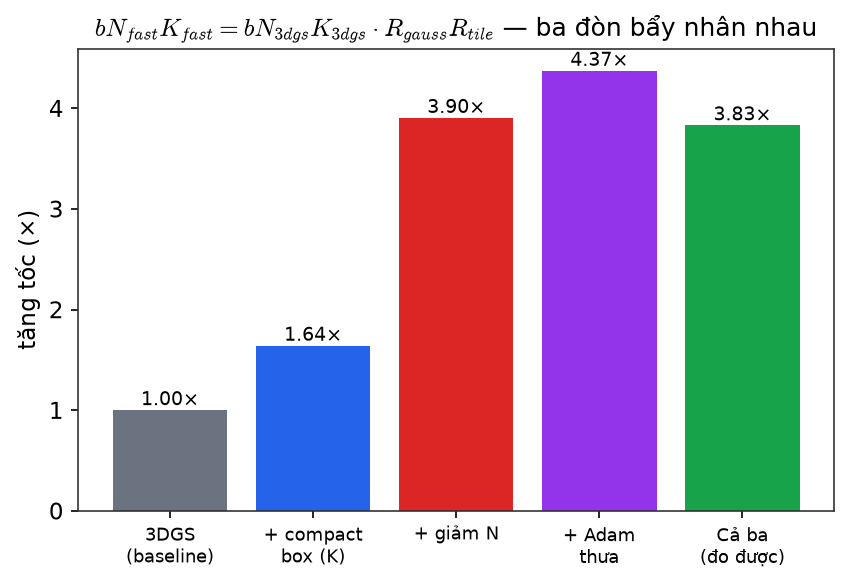
\includegraphics[width=0.68\linewidth]{ch8_levers_waterfall.png}
\end{center}
\end{frame}
   % Slide 29-32 Tổng kết 5 cải tiến, Vì sao 3DGS chậm, 3 đòn bẩy, Thác nước
% ===== FILE 9/9: Toàn cảnh lịch trình, Chi phí trung thực, Bảng đang chạy, Bảng so sánh, Ưu điểm, Tổng kết, Cảm ơn =====

% --- Slide: Toàn cảnh lịch trình huấn luyện ---
\begin{frame}{Toàn cảnh lịch trình huấn luyện ($30\,000$ iteration)}
\scriptsize
\begin{center}
\begin{tabular}{lll}
\toprule
\textbf{Mốc} & \textbf{Sự kiện} & \textbf{Ghi chú}\\
\midrule
iter $1\to3$ & tăng bậc SH tới $D_{\max}=3$ & mỗi iteration\\
iter $500$ & bắt đầu densify & \texttt{densify\_from\_iter}\\
iter $600,700,\dots$ & clone/split/prune ($\eta$ OR gradient) & mỗi $100$, tới iter $15\,000$\\
iter $3\text{k},6\text{k},9\text{k},12\text{k}$ & reset opacity ($\times0.1$) & đúng $4$ lần, chỉ khi $<15\,000$\\
iter $4\,000$, $8\,000$ & prune cứng thêm ($\alpha<0.1$) & \texttt{prune\_iterations}\\
iter $15\,000$ & \textbf{dừng hẳn} densify/prune/reset & \texttt{densify\_until\_iter}\\
iter $15\,000\to30\,000$ & chỉ còn tối ưu Adam, $N$ không đổi & ---\\
\bottomrule
\end{tabular}
\end{center}
\begin{itemize}\itemsep1pt
    \item \textbf{Không có} cơ chế nào chủ động thay đổi $N$ sau iteration $15\,000$ --- toàn bộ số lượng Gaussian đạt
    được tại mốc đó được giữ nguyên cho tới hết quá trình train, chỉ còn tối ưu giá trị tham số.
    \item Đây là điểm quan trọng khi so sánh 3DGS gốc với SADGS: khác biệt về \textbf{chất lượng/tốc độ hội tụ} chủ yếu
    xảy ra trong $15\,000$ iteration đầu, không phải "số Gaussian cuối cùng khác nhau nhờ tiếp tục tỉa về sau".
\end{itemize}
\end{frame}

% --- Slide: Mô hình chi phí — trung thực ---
\begin{frame}{Chi phí tính toán: mô hình định tính, KHÔNG có số đo thật}
\scriptsize
Repo này \textbf{không chứa} script benchmark thời gian thực (wall-clock) nào đo trực tiếp và so sánh SADGS với 3DGS
gốc trên cùng phần cứng, cùng scene, cùng số lần lặp lại đo. Một mô hình \textbf{định tính} hợp lý (không phải số đo
thực nghiệm) cho chi phí mỗi iteration:
\[
T_{\text{iter}} \approx a\,N \;+\; b\,N\,K \;+\; c\,N\cdot\mathbb{1}[\text{Adam step}] \;+\; F
\]
với $N$ số Gaussian, $K$ số tile trung bình/Gaussian (bị chi phối bởi \texttt{mult} của compact box), $F$ chi phí cố
định mỗi khung hình (forward pass loss, sắp xếp, v.v.).
\begin{itemize}\itemsep1pt
    \item Thành phần \textbf{có thể làm tăng} chi phí/iteration so với đường cơ sở: cập nhật $\eta$ mỗi $10$ iteration
    (thêm một lượt tính structure tensor và chiếu trục), hai optimizer chạy song song trong chế độ \texttt{hybrid}.
    \item Thành phần \textbf{có thể làm giảm} chi phí: \texttt{mult}$=0.7<1$ giảm $K$ so với SnugBox nguyên bản
    (\texttt{mult}$=1$) --- ít tile hơn cho mỗi Gaussian.
    \item \textbf{Nguyên tắc trình bày của bài giảng này:} bất kỳ con số "nhanh hơn $X$ lần", "giây/iteration" nào không
    đi kèm phương pháp đo rõ ràng (phần cứng cụ thể, scene cụ thể, số lần lặp lại đo) sẽ \textbf{không được trích dẫn}
    như một kết quả benchmark đã kiểm chứng.
\end{itemize}
\end{frame}

% --- Slide: Bảng những gì đang thật sự chạy mặc định ---
\begin{frame}{Tóm tắt: những gì ĐANG CHẠY mặc định trong repo này}
\scriptsize
\begin{center}
\begin{tabular}{ll}
\toprule
\textbf{Cơ chế} & \textbf{Vị trí trong code}\\
\midrule
Structure tensor đa tỉ lệ $\to\eta\to$ split/clone/prune & \texttt{utils/freq\_utils.py}, \texttt{train.py:276,341--372}\\
Split dị hướng $k_x k_y k_z$ theo từng trục & \texttt{scene/gaussian\_model.py:638}\\
Tích luỹ nhất quán đa view (high/low ratio) & \texttt{train.py:341--353}\\
Reset opacity $\times0.1$, đúng $4$ lần & \texttt{scene/gaussian\_model.py:415}\\
Trần opacity $\min(\alpha,0.8)$ & \texttt{scene/gaussian\_model.py:1043}\\
Optimizer hybrid (Adam thường $+$ Sparse/Fused Adam) & \texttt{train.py:429--434}\\
Compact box SnugBox, \texttt{mult}$=0.7$ & \texttt{cuda\_rasterizer/auxiliary.h:313}\\
Bộ lọc low-pass 2D, $\kappa=0.1$ & \texttt{cuda\_rasterizer/forward.cu:113}\\
\bottomrule
\end{tabular}
\end{center}
\footnotesize Đây là danh sách đầy đủ những gì bài giảng này đã trình bày chi tiết --- các nhánh tuỳ chọn khác trong
code (nhánh 3DGS gốc dùng làm baseline so sánh ở phần đầu, và một vài cơ chế được thiết kế nhưng hiện đang tắt theo
mặc định) không được đào sâu thêm ở đây vì không ảnh hưởng tới hành vi mặc định của pipeline.
\end{frame}

% --- Slide: Bảng so sánh 3DGS gốc / SADGS (chỉ những khác biệt đang thật sự chạy) ---
\begin{frame}{Bảng so sánh 3DGS gốc vs.\ SADGS (chỉ những khác biệt ĐANG CHẠY)}
\scriptsize
\begin{center}
\begin{tabular}{p{4.6cm}p{3.6cm}p{4.4cm}}
\toprule
\textbf{Tiêu chí} & \textbf{3DGS gốc (baseline)} & \textbf{SADGS (mặc định)}\\
\midrule
Tín hiệu densify chính & gradient vị trí & gradient \textbf{OR} $\eta$ tần số đa tỉ lệ\\
Split dị hướng theo trục & không có (luôn $N{=}2$, mọi trục $/1.6$) & có, $k_{\text{axis}}=\lceil\sqrt{\max(\eta,1)}\rceil$ riêng từng trục\\
Tích luỹ đa view trước quyết định & không (đọc gradient tại 1 lần cuối) & có (\texttt{high\_ratio}/\texttt{low\_ratio}$>0.8$ qua nhiều view)\\
Vị trí Gaussian con khi split & ngẫu nhiên $\mathcal{N}(0,\mathrm{diag}(s)^2)$ & lưới tất định, cách đều $\sqrt{12}\sigma$\\
\bottomrule
\end{tabular}
\end{center}
\footnotesize\textit{Compact box, bộ lọc low-pass 2D và optimizer hybrid là các cơ chế \textbf{chạy giống nhau} ở cả hai
nhánh (xem slide "kế thừa vs mới") --- không đưa vào bảng so sánh vì không phải điểm khác biệt.}
\end{frame}

% --- Slide: Ưu điểm cốt lõi ---
\begin{frame}{Ưu điểm cốt lõi của SADGS: hội tụ đúng chỗ, không phải "ít Gaussian hơn"}
\scriptsize
\begin{itemize}\itemsep2pt
    \item \textbf{Đừng diễn giải sai:} không có bằng chứng trong repo cho thấy SADGS tạo ra \textbf{ít Gaussian hơn} so
    với 3DGS gốc ở cùng mức chất lượng --- cơ chế duy nhất có khả năng chủ động giảm mạnh $N$ ở giai đoạn cuối không
    nằm trong phạm vi những gì đang chạy mặc định (xem slide "đang chạy mặc định").
    \item \textbf{Lợi ích thực sự, có căn cứ trực tiếp từ công thức đã trình bày:}
    \begin{itemize}
        \item Phân bổ ngân sách split \textbf{đúng trục, đúng mức độ} ($k_{\text{axis}}$ tính riêng từng trục, tăng
        theo bậc thang tương xứng với mức độ vi phạm) thay vì luôn chia đôi đều mọi trục như cơ chế gốc.
        \item Quyết định dựa trên \textbf{đa số view đồng thuận} ($>80\%$), giảm hẳn nguy cơ phản ứng theo nhiễu của một
        góc chụp đơn lẻ bất thường.
        \item Tín hiệu $\eta$ đo trực tiếp \textbf{tỉ lệ kích thước Gaussian / chi tiết ảnh}, bổ sung cho gradient (vốn
        chỉ phản ánh trạng thái hội tụ hiện tại, và có thể bị triệt tiêu nội-ảnh giữa các pixel như đã học).
    \end{itemize}
    \item \textbf{Còn bỏ ngỏ, cần nói rõ khi trình bày kết quả:} repo không có số đo PSNR/SSIM/LPIPS hay wall-clock nào
    so sánh trực tiếp hai nhánh trên cùng scene/checkpoint để \textbf{định lượng} các lợi ích lý thuyết vừa nêu.
\end{itemize}
\end{frame}

% --- Slide: Tổng kết ---
\begin{frame}{Tổng kết: từ 3DGS gốc tới SADGS}
\scriptsize
\begin{enumerate}\itemsep2pt
    \item \textbf{Biểu diễn \& render:} Gaussian 3D tường minh, EWA splatting, alpha blending, rasterizer theo tile ---
    nền tảng chung, giữ nguyên giữa hai nhánh.
    \item \textbf{Gradient:} tích luỹ đúng cách (chuẩn trước, cộng sau) tránh triệt tiêu giữa các view; vấn đề triệt
    tiêu thật nằm giữa các pixel trong cùng một ảnh, được xử lý bằng một kênh gradient trị tuyệt đối riêng.
    \item \textbf{ADC gốc:} clone/split/prune dựa thuần trên gradient --- khung sườn chung mà SADGS kế thừa nguyên vẹn.
    \item \textbf{SADGS:} bổ sung tín hiệu $\eta$ (tỉ số kích thước Gaussian / bước sóng texture cục bộ), tích luỹ nhất
    quán qua nhiều view, split dị hướng theo đúng trục vi phạm --- kết hợp \texttt{OR} với gradient chứ không thay thế,
    và đây là phần \textbf{đang chạy mặc định}.
    \item \textbf{Trung thực về hiệu năng:} không có số đo wall-clock/chất lượng nào trong repo để khẳng định "nhanh
    hơn" hay "ít Gaussian hơn" một cách định lượng --- bài giảng này trình bày đúng những gì công thức và code thể
    hiện, không suy diễn thêm ngoài đó.
\end{enumerate}
\end{frame}

% --- Slide: Cảm ơn / Q&A ---
\begin{frame}{Cảm ơn}
\centering
\vspace{1cm}
{\Large Câu hỏi \& thảo luận}\\[0.8cm]
\footnotesize
Toàn bộ công thức trong bài giảng này được đối chiếu trực tiếp với:\\
\texttt{train.py}, \texttt{scene/gaussian\_model.py}, \texttt{utils/freq\_utils.py}, \texttt{utils/loss\_utils.py},\\
\texttt{arguments/\_\_init\_\_.py}, \texttt{cuda\_rasterizer/\{forward.cu, auxiliary.h\}} và \texttt{DOCS/BOOK/}.
\end{frame}
   % Slide 33-38 Cơ chế lõi structure-aware/eta, Colab T4, các bảng số
% ============================================================
% PHẦN SADGS (bản 45 phút, rút gọn) — 3 slide
% Rút gọn từ part_sadgs_01.tex..08.tex (bản full, ../part_sadgs_*.tex)
% Slide C (mới): bảng tổng kết so sánh 3DGS gốc (densify_and_clone/split,
% scene/gaussian_model.py) / SADGS, đối chiếu với cơ chế lõi structure-aware
% đã trình bày ở part45_09.tex Slide 33.
% ============================================================

% --- Slide C (MỚI) ---
\begin{frame}{Bảng tổng kết: 3DGS gốc (vanilla) vs.\ SADGS (mới)}
\footnotesize
\begin{table}
\centering
\begin{tabular}{lcc}
\toprule
\textbf{Cơ chế} & \textbf{3DGS gốc (\texttt{densify\_and\_clone/split})} & \textbf{SADGS (mới)} \\
\midrule
Đo độ khớp kích thước & không có & $\eta = \dfrac{\text{trục chiếu}}{\text{bước sóng texture}}$ \\
Ngưỡng phân loại & -- & $\tau_{\text{high}}{=}1.0$, $\tau_{\text{low}}{=}0.1$ \\
Split & luôn 2 con, ngẫu nhiên & dị hướng theo trục, $k_{\text{axis}}{=}\lceil\sqrt{\eta_{\text{axis}}}\rceil$ \\
Giãn Gaussian dưới cỡ & không có & \texttt{expand\_undersized\_gs}$^\dagger$ \\
Prune cuối & không có & \texttt{final\_prune\_structgs}$^\dagger$ \\
\bottomrule
\end{tabular}
\end{table}
{\scriptsize $^\dagger$ Đã cài đặt đúng trong \texttt{gaussian\_model.py} nhưng lời gọi đang bị comment out trong \texttt{train.py} -- không chạy mặc định (xem Slide 33, 41). Cột 3DGS gốc lấy trực tiếp từ \texttt{densify\_and\_clone}/\texttt{densify\_and\_split} trong \texttt{scene/gaussian\_model.py}.}
\end{frame}
   % Slide C     Bảng so sánh 3 phương pháp

\section{SADGS chuyên sâu}
% ===== BOT 00: Bản đồ toàn tuyến Structure Tensor -> ADC (bản 45 phút) =====
% Đặt TRƯỚC part45_sadgsx_01 để dẫn đường cho 15 slide chuyên sâu.
% Hình: ../figures/sadgsx/scripts/bot16_figs.py

\begin{frame}{Bản đồ 15 slide tới: từ \emph{structure tensor} đến \emph{ADC}}
\scriptsize
\vspace{-3mm}
\begin{center}
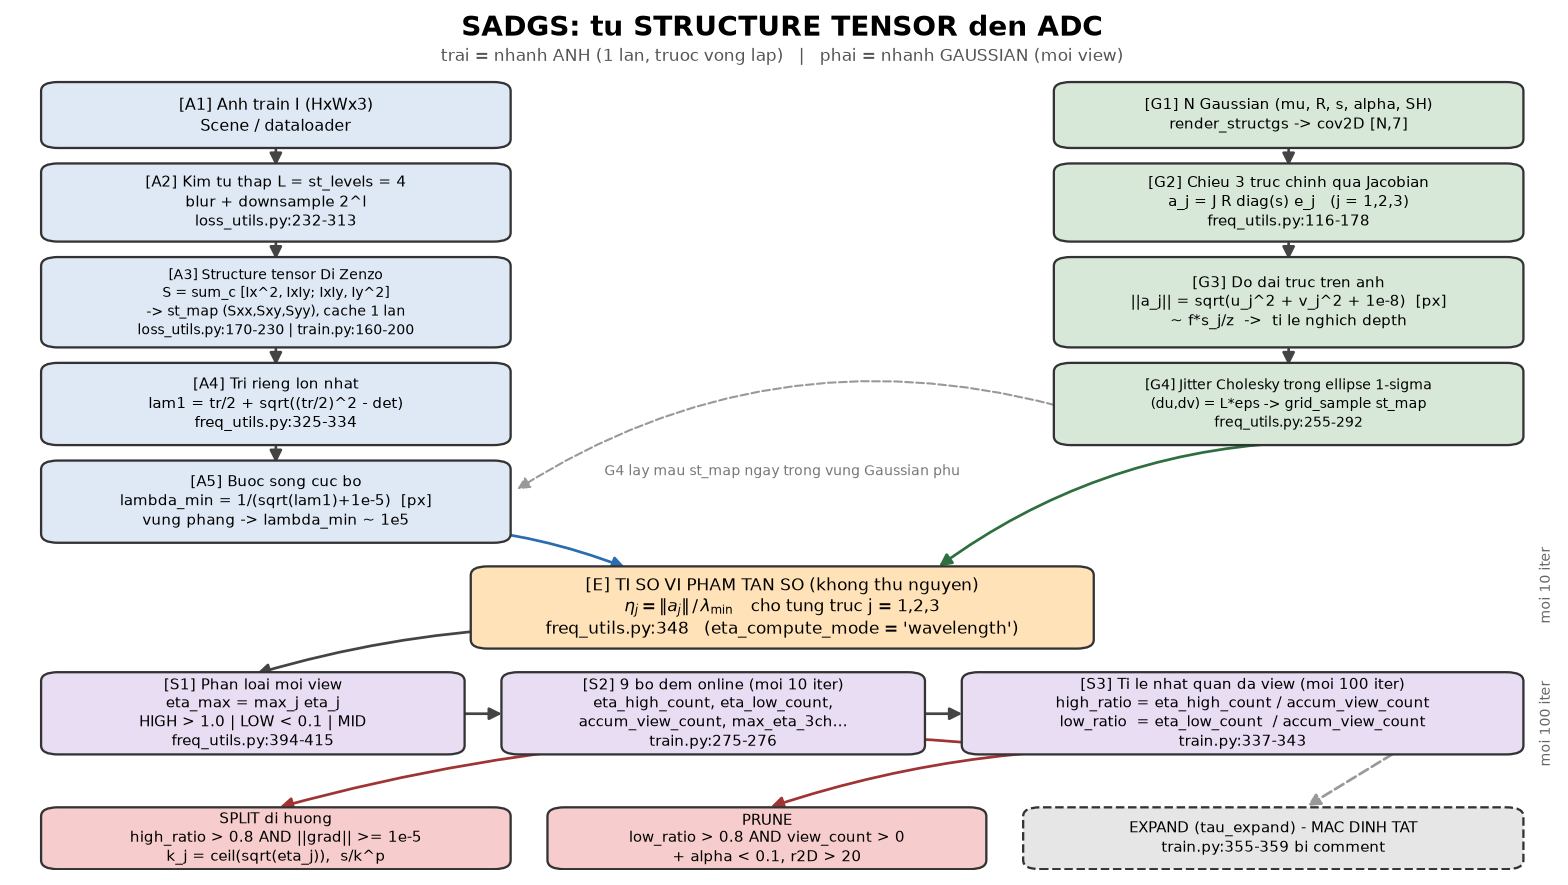
\includegraphics[width=0.80\linewidth]{sadgsx/16_flow_tensor_to_adc.png}
\end{center}
\vspace{-2mm}
\captionof{figure}{\scriptsize Nhánh \textbf{ảnh} (xanh dương) chạy một lần trước vòng lặp $\to$ $\lambda_{\min}$; nhánh \textbf{Gaussian} (xanh lá) chạy mỗi view $\to$ $\|a_j\|$. Hai nhánh gặp nhau đúng một chỗ: $\eta_j=\|a_j\|/\lambda_{\min}$ (ô cam). Tím = bỏ phiếu đa view, hồng = ADC, xám nét đứt = mặc định TẮT.}
\end{frame}

\begin{frame}{Ba điều cần nhớ trước khi đi vào chi tiết}
\scriptsize
\vspace{-3mm}
\begin{columns}[T]
\begin{column}{0.5\textwidth}
\begin{enumerate}
    \item \textbf{$\eta$ là tỉ số không thứ nguyên} (pixel/pixel) --- nhờ vậy hai ngưỡng hằng $\tau_{high}{=}1.0$, $\tau_{low}{=}0.1$ mới dùng được xuyên cảnh.
    \item \textbf{Giữ ba $\eta$, không phải một} --- ba trục chính của ellipsoid, nhờ đó mới chia \emph{dị hướng} được: $k_j=\lceil\sqrt{\max(\eta_j,1)}\rceil$.
    \item \textbf{Đo tách khỏi quyết định} --- đo mỗi 10 iteration, quyết định mỗi 100 iteration bằng \texttt{high\_ratio}/\texttt{low\_ratio} so với $0.8$.
\end{enumerate}
\vspace{1mm}
\alert{Cổng AND} (\texttt{train.py:345}) là chốt chặn chống bùng nổ $N$:
\[
\texttt{split} = (\texttt{high\_ratio}{>}0.8) \wedge (\|\nabla_{\mathbf{x}_{2D}}\mathcal{L}\|{\ge}10^{-5})
\]
\end{column}
\begin{column}{0.48\textwidth}
\begin{center}
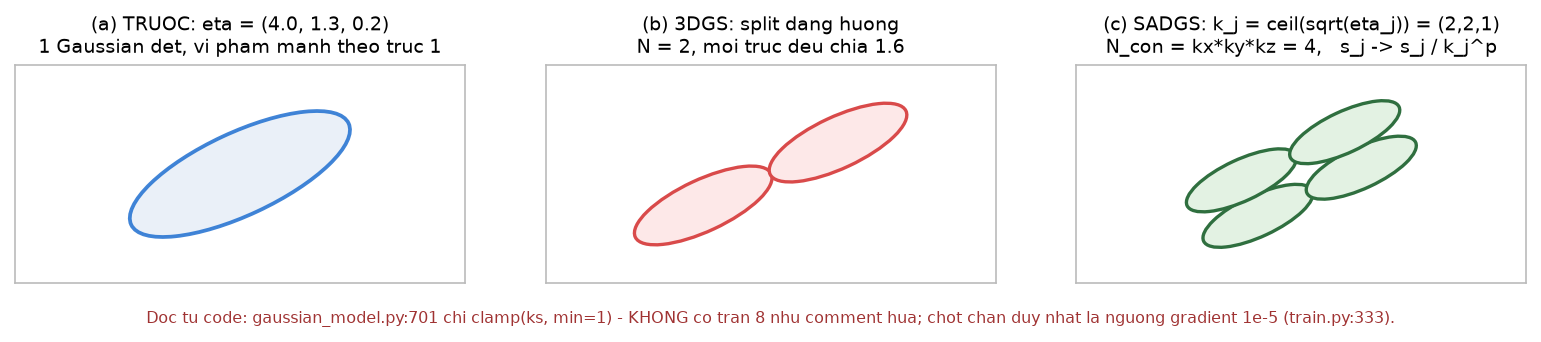
\includegraphics[width=\linewidth]{sadgsx/16_adc_actions.png}\\[3pt]
\captionof{figure}{\scriptsize 3DGS chia đều mọi trục cho 1.6; SADGS chia riêng từng trục theo $\eta_j$ rồi thu scale $s_j/k_j^{\,p}$.}
\end{center}
\end{column}
\end{columns}
\end{frame}
   % Bản đồ toàn tuyến: Structure Tensor -> ADC (2 slide)
% ===== BOT 01: Structure tensor & multiscale image structure (bản 45 phút) =====

\begin{frame}{Tensor cấu trúc đa tỉ lệ — nền tảng đo cấu trúc ảnh của SADGS}
\scriptsize
\begin{columns}[T]
\begin{column}{0.46\textwidth}
\[
J_\rho=G_\rho*\!\begin{bmatrix} \sum_c I_{x,c}^2 & \sum_c I_{x,c}I_{y,c}\\ \sum_c I_{x,c}I_{y,c} & \sum_c I_{y,c}^2\end{bmatrix}
\]
\[
\lambda_{1,2}=\frac{\mathrm{tr}}{2}\pm\sqrt{\Big(\frac{\mathrm{tr}}{2}\Big)^2-\det},\quad
w_{\min}=\frac{1}{\sqrt{\lambda_1}}
\]
\[
\hat J=\frac{\sum_i \dfrac{J_i}{\mathrm{tr}J_i}\,b_i^{\,p}\,f_i^{2}}{\sum_i b_i^{\,p}+10^{-6}},\quad
\sigma_i=\sigma_0 s^i,\ f_i=s^{-i}
\]
\begin{itemize}
\item Sobel sau làm mượt, cộng năng lượng 3 kênh RGB (Di Zenzo) — \texttt{loss\_utils.py:170--230}.
\item $\lambda_1$ $\to$ bước sóng nhỏ nhất (px); $v_2\perp v_1$ $\to$ hướng texture.
\item Đa tỉ lệ: $b_i$ là DoG, $\rho_i=3\sigma_i$; mặc định \texttt{levels=4}, $\sigma_0{=}1$, $s{=}1.5$, $p{=}3$.
\item \textbf{v1} (\texttt{:282}) làm mờ lại tensor gốc; \textbf{v2} (\texttt{:357}) tính lại tensor trên ảnh đã mờ ở từng thang. Mặc định \texttt{st\_mode="v1"}.
\item \texttt{st\_map} $(1,3,H,W)=(S_{xx},S_{xy},S_{yy})$, cache theo \texttt{image\_name} một lần trước khi train (\texttt{train.py:160--200}).
\end{itemize}
\end{column}
\begin{column}{0.54\textwidth}
\begin{center}
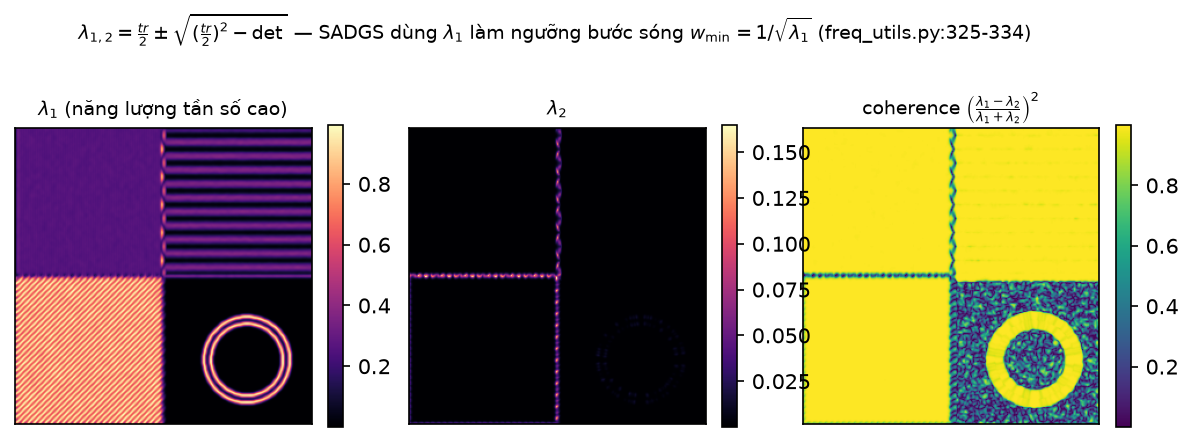
\includegraphics[width=\linewidth]{sadgsx/01_eigen_coherence.png}\\[2pt]
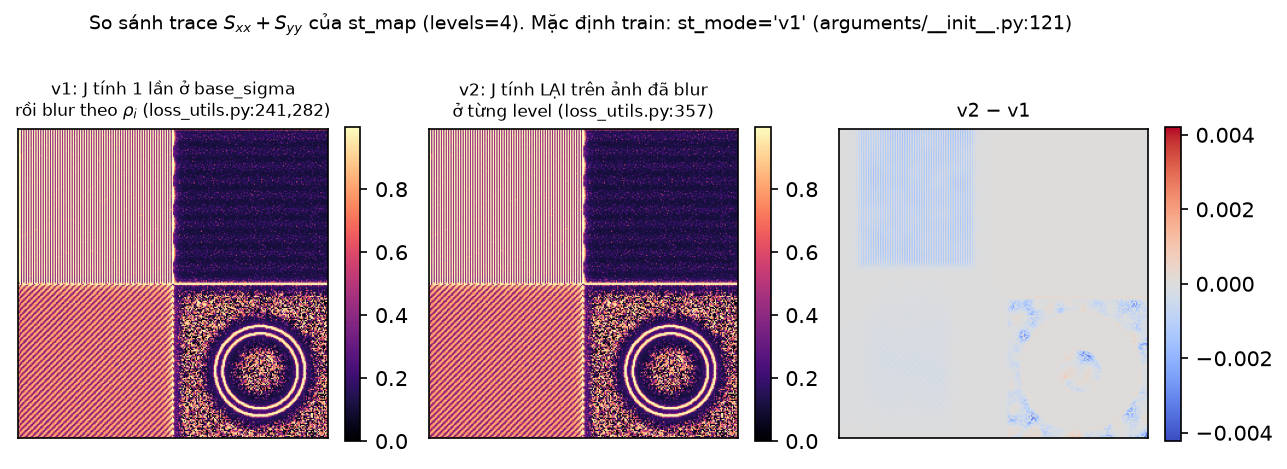
\includegraphics[width=\linewidth]{sadgsx/01_v1_vs_v2.png}
\captionof{figure}{\scriptsize Trên: $\lambda_1,\lambda_2$, coherence. Dưới: trace \texttt{st\_map} theo v1 vs v2.}
\end{center}
\end{column}
\end{columns}
\end{frame}

% ===== BOT 02: Chiếu trục Gaussian lên màn hình & tỉ số cấu trúc eta =====

\begin{frame}{SADGS --- Tỉ số cấu trúc $\eta$: Gaussian có "quá to" so với texture?}
\scriptsize
\begin{columns}[T]
\begin{column}{0.46\textwidth}
\textbf{1. Chiếu 3 trục xuống màn hình}\\
(\texttt{freq\_utils.py:116--178})
\[
A_{cam}=R_{view}R(r)\,\mathrm{diag}(s),\quad
\begin{aligned}
u_j&=J_{00}A^x_j+J_{02}A^z_j\\
v_j&=J_{11}A^y_j+J_{12}A^z_j
\end{aligned}
\]
với $J$ có hàng $u=(f_x/z,0,-f_xx/z^2)$, hàng $v=(0,f_y/z,-f_yy/z^2)$; depth $z$, tâm
\texttt{means2D} lấy từ \texttt{cov2D} của rasterizer.
\[
\|a_j\|=\sqrt{u_j^2+v_j^2+10^{-8}}\ \ [\text{pixel}]\ \propto f s_j/z
\]

\textbf{2. Bước sóng cục bộ} (fu:325--334)
\[
\lambda_1=\tfrac{\mathrm{tr}}{2}+\sqrt{(\tfrac{\mathrm{tr}}{2})^2-\det},\quad
\lambda_{\min}=\tfrac{1}{\sqrt{\lambda_1}+10^{-5}}
\]

\textbf{3. Tỉ số} (\texttt{eta\_compute\_mode="wavelength"}, fu:348)
\[
\boxed{\ \eta_j=\|a_j\|/\lambda_{\min}\ }\quad j=1,2,3\ \text{(3 trục chính)}
\]
$\eta_{\max}>\tau_{high}=1.0\Rightarrow$ \textbf{SPLIT};
$\eta_{\max}\le\tau_{low}=0.1\Rightarrow$ \textbf{PRUNE} (fu:395--409),
chốt khi tỉ lệ đa view $>0.8$ (\texttt{train.py:345,353}).
\end{column}
\begin{column}{0.52\textwidth}
\begin{center}
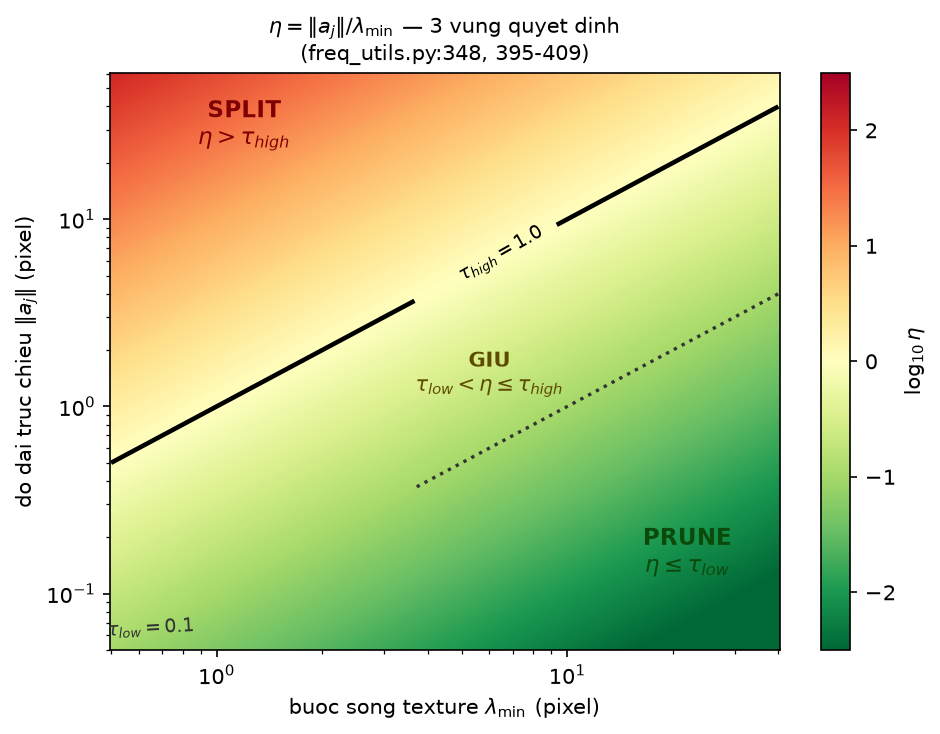
\includegraphics[width=0.92\linewidth]{sadgsx/02_eta_heatmap.png}\\
\captionof{figure}{\tiny $\eta$ trên lưới (độ dài trục chiếu) $\times$ (bước sóng texture): 3 vùng SPLIT / GIỮ / PRUNE. Trực giác Nyquist --- Gaussian rộng hơn chu kỳ texture thì xoá mất chi tiết.}
\end{center}
\end{column}
\end{columns}
\end{frame}

% ===== BOT 03: Thống kê eta online đa view \& tỉ lệ nhất quán (multiview consistency ratio) =====

\begin{frame}{SADGS --- Tỉ lệ nhất quán đa view cho densify/prune}
\scriptsize
\begin{columns}[T]
\begin{column}{0.5\linewidth}
$\eta$ (mức vi phạm tần số) phụ thuộc view $\Rightarrow$ \textbf{không} quyết định trên 1 view. Mỗi 10 iteration, \texttt{update\_freq\_stats\_online} (\texttt{utils/freq\_utils.py:181}) tích luỹ bộ đếm cho từng Gaussian, chỉ với mẫu qua bộ lọc
\[
(T_{\max}>0)\wedge(\alpha>0.05)\wedge(\|\nabla_{xy}\|>2\!\times\!10^{-5})
\]
Phân loại mỗi quan sát theo $\eta_{\max}=\max_k \eta_k$: HIGH nếu $>\tau_{high}{=}1.0$, LOW nếu $\le\tau_{low}{=}0.1$ (\texttt{freq\_utils.py:395--409}).

Mỗi \texttt{densification\_interval}$=100$ iter (\texttt{train.py:337--353}):
\[
r^{high}=\frac{\texttt{eta\_high\_count}}{\texttt{accum\_view\_count}},\quad
r^{low}=\frac{\texttt{eta\_low\_count}}{\texttt{accum\_view\_count}}
\]
\[
\texttt{SPLIT}: r^{high}>0.8 \wedge \|\bar g\|\ge 10^{-5};\quad
\texttt{PRUNE}: r^{low}>0.8
\]
Kích thước con định hình bằng \texttt{max\_eta\_3ch} (worst-case qua view), không dùng trung bình. Sau densify, cả 9 bộ đếm \texttt{zero\_()} (\texttt{train.py:377--386}) $\Rightarrow$ cửa sổ trượt $\approx 10$ mẫu/chu kỳ.
\end{column}
\begin{column}{0.5\linewidth}
\centering
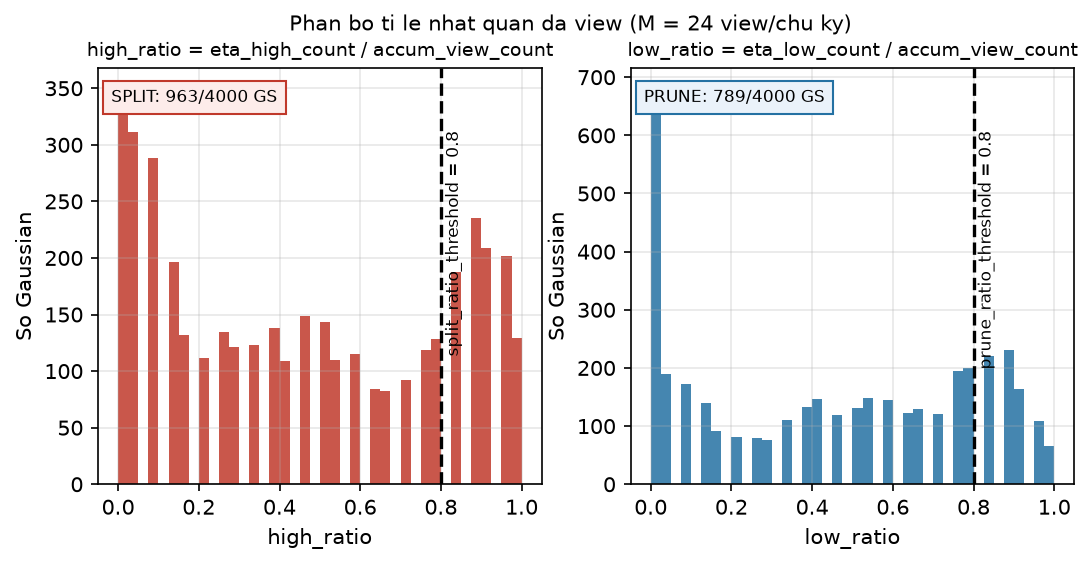
\includegraphics[width=\linewidth]{sadgsx/03_ratio_hist.png}

\vspace{2pt}
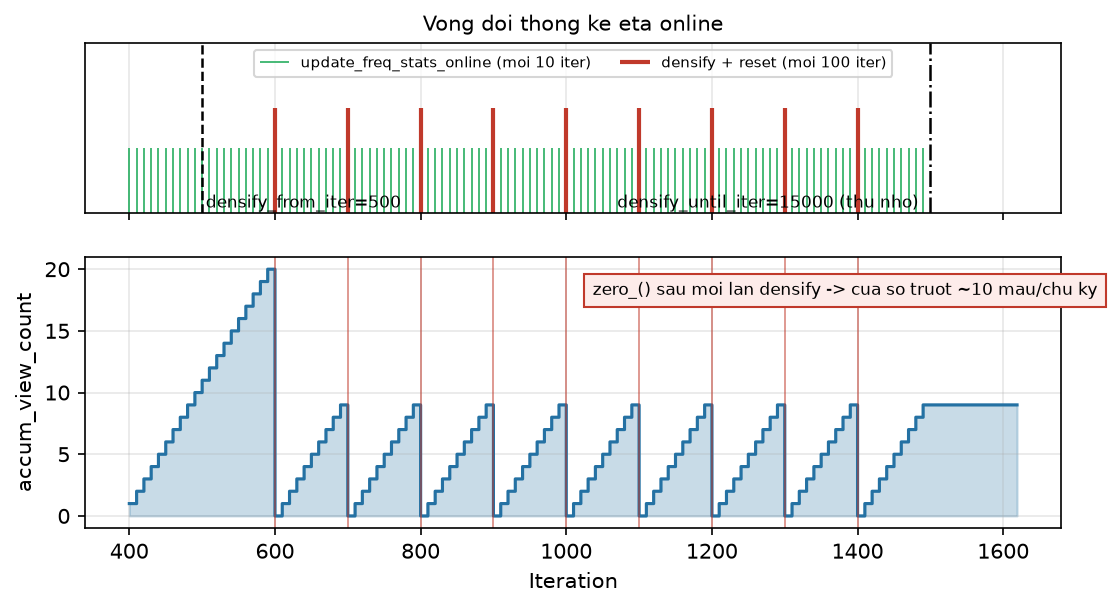
\includegraphics[width=\linewidth]{sadgsx/03_timeline_reset.png}
\captionof{figure}{\scriptsize Trên: phân bố $r^{high}$/$r^{low}$ và ngưỡng $0.8$. Dưới: vòng đời cập nhật (mỗi 10 iter) --- densify + reset (mỗi 100 iter).}
\end{column}
\end{columns}
\end{frame}

% ===== BOT 04: densify_and_split_structgs — split dị hướng theo từng trục =====

\begin{frame}{SADGS: tách Gaussian \textbf{dị hướng} theo từng trục (\texttt{densify\_and\_split\_structgs})}
\scriptsize
\begin{columns}[T]
\begin{column}{0.44\linewidth}
\textbf{Ba công thức cốt lõi} \tiny(\texttt{scene/gaussian\_model.py:638--832})\scriptsize
\[
k_a=\max\!\Big(1,\big\lceil\sqrt{\max(\eta_a,1)}\big\rceil\Big)\ \ \text{\tiny(699--701)}
\]
\[
N=k_xk_yk_z\ \ \text{\tiny(714)},\qquad
\sigma'_a=\frac{\sigma_a}{k_a^{\,p}}\ \ \text{\tiny(722)}
\]
\[
\mathbf{x}_{\text{con}}=\mathbf{x}_{\text{cha}}+R(q)\Big[\sqrt{12}\,\tfrac{\boldsymbol\sigma}{\mathbf{k}}\odot\Big(\mathbf{i}-\tfrac{\mathbf{k}-1}{2}\Big)\Big]\ \text{\tiny(763--788)}
\]
\begin{itemize}
  \item $\eta_a$ = năng lượng tần số vượt Nyquist trên trục $a$ $\Rightarrow$ \textbf{trục nào aliasing nhiều thì cắt nhiều}, trục đủ mịn giữ $k=1$.
  \item Con nằm trên \textbf{lưới đều tất định} trong hệ local rồi xoay bằng $R(q)$; hệ số $\sqrt{12}$ giữ phương sai cha.
  \item Kế thừa nguyên vẹn rotation, SH, \textbf{opacity không giảm}, \texttt{tmp\_radii}, \texttt{filter\_3D}; \texttt{densify\_count}$+1$. Cha bị \texttt{prune\_points} xoá sau khi thêm con (807--831).
  \item So với 3DGS gốc (\texttt{:866--892}): luôn $N{=}2$, tâm \textbf{ngẫu nhiên} $\mathcal{N}(0,\Sigma)$, $\sigma'=\sigma/1.6$ cho \textbf{mọi} trục.
  \item \alert{Chú thích dòng 698 nói ``clamp max=8'' nhưng code chỉ \texttt{clamp(min=1)}} --- $k$ không có trần.
\end{itemize}
\end{column}
\begin{column}{0.55\linewidth}
\centering
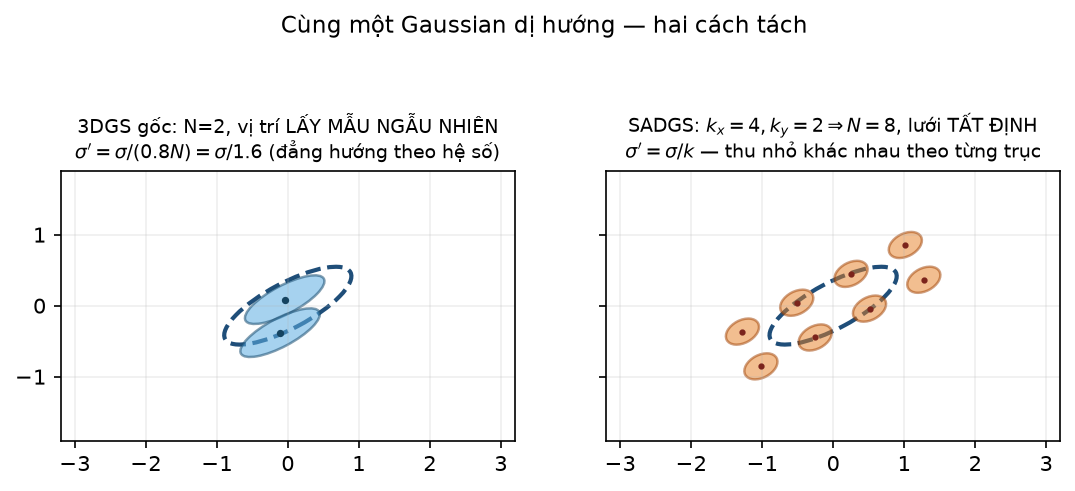
\includegraphics[width=0.99\linewidth]{sadgsx/04_3dgs_vs_sadgs.png}
\captionof{figure}{\tiny Cùng một Gaussian dị hướng. Trái: 3DGS gốc, 2 con ngẫu nhiên, vẫn dài theo trục vi phạm. Phải: SADGS $k_x{=}4,k_y{=}2\Rightarrow N{=}8$ con trên lưới tất định, mỗi trục co đúng hệ số cần thiết.}
\end{column}
\end{columns}
\end{frame}

% ===== BOT 05: densify_and_clone_structgs & cơ chế ghép tensor vào optimizer =====

\begin{frame}{Clone trong SADGS và cách ghép tensor vào optimizer}
\scriptsize
\begin{columns}[T]
\begin{column}{0.52\textwidth}
\textbf{1. Chọn điểm} (\texttt{gaussian\_model.py:935, 998--1007}):
\[
\mathcal{S}=\underbrace{(\texttt{acc\_view\_cnt}>0.5)}_{\texttt{metric\_mask}}\wedge\big(\texttt{eta\_mask}\vee\|\bar g\|\!\ge\!\tau_g\big)\wedge\big(\max_i s_i\!\le\!\lambda_d\,\text{ext}\big)
\]
$\tau_g=2\times10^{-4}$, $\lambda_d=\texttt{args.dense}=0.001$ (\texttt{arguments:112--113}). Khác 3DGS (\texttt{:895--897}): tiêu chí đến \emph{từ ngoài}, có nhánh tần số đa view, ngưỡng scale chặt hơn $10\times$.

\textbf{2. Sao chép nguyên xi} (\texttt{:937--944}): $\mu_{new}=\mu_{old}$, không dịch vị trí, không chia scale; \texttt{densify\_count} kế thừa (\texttt{:952--954}).

\textbf{3. Ghép vào Adam} (\texttt{:578--586}):
\[
\theta'=\mathrm{cat}(\theta,\theta[\mathcal{S}]),\quad m'=\mathrm{cat}(m,\mathbf{0}_M),\quad v'=\mathrm{cat}(v,\mathbf{0}_M)
\]
Phải \texttt{del opt.state[p]} $\to$ tạo \texttt{nn.Parameter} mới $\to$ gán lại state, vì khoá của \texttt{opt.state} chính là đối tượng \texttt{Parameter}.

\textbf{4. Hệ quả reset moment:} bước đầu của điểm mới $\approx\frac{1-\beta_1}{\sqrt{1-\beta_2}}=3.16$ lần bước thường — chính cú hích này tách hai bản sao trùng khít ra khỏi nhau.
\end{column}
\begin{column}{0.46\textwidth}
\begin{center}
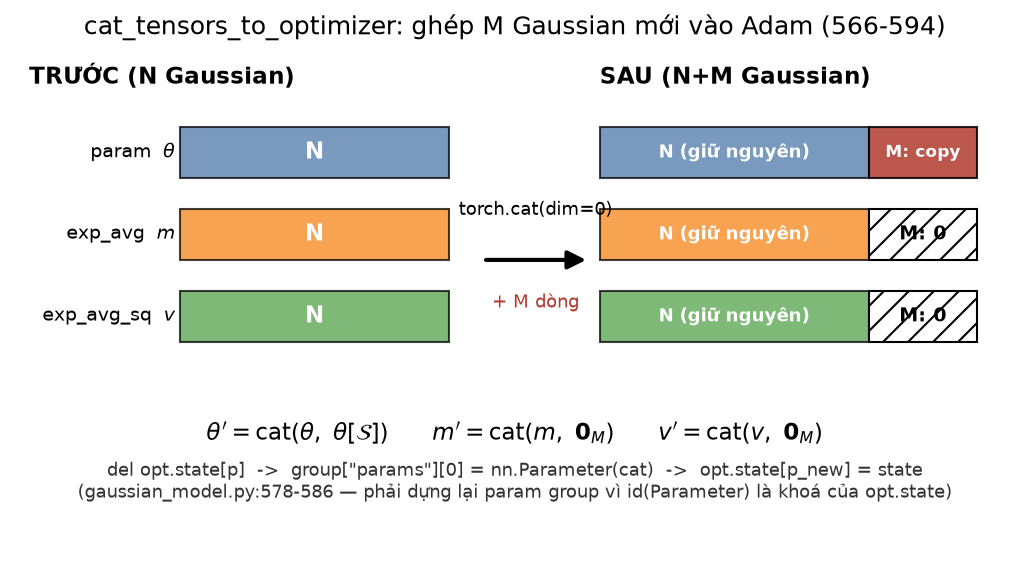
\includegraphics[width=\linewidth]{sadgsx/05_cat_tensor_optimizer.png}
\captionof{figure}{\scriptsize Chiều tensor $N\to N+M$: tham số được sao chép, hai moment Adam khởi tạo 0 (\texttt{cat\_tensors\_to\_optimizer}, \texttt{:566--594}).}
\end{center}
\end{column}
\end{columns}
\end{frame}

% ===== BOT 06: expand_undersized_gs — giãn giải tích Gaussian dưới cỡ (bản 45 phút) =====

\begin{frame}{Giãn giải tích Gaussian dưới cỡ (\texttt{expand\_undersized\_gs}) --- và trạng thái \emph{bị tắt}}
\scriptsize
\begin{columns}[T]
\begin{column}{0.47\textwidth}
Gaussian có $\eta=\ell_{\text{truc}}/\lambda_{\min}<\tau_{expand}$ là \textbf{nhỏ hơn} chi tiết texture $\Rightarrow$ lãng phí điểm. SADGS sửa \textbf{trực tiếp} tham số thay vì sinh thêm Gaussian:
\[
\texttt{mask}=(\eta<\tau_{expand})\wedge(\eta>0),\quad \tau_{expand}=1.0
\]
\[
\Delta_{\log}=-\tfrac12\ln\!\big(\max(\eta,10^{-6})\big)
\ \Rightarrow\ \frac{s_{\text{mới}}}{s_{\text{cũ}}}=\eta^{-1/2}
\]
\begin{itemize}\itemsep1pt
    \item Cộng thẳng vào log-scale vì $\sigma=\exp(\texttt{\_scaling})$; $N$ \textbf{không đổi} $\Rightarrow$ $0$ byte thêm (so với split cần $k^3$ Gaussian, $k=\lceil\eta^{-1/2}\rceil$).
    \item Ghi qua \texttt{replace\_tensor\_to\_optimizer(\dots,"scaling")} $\Rightarrow$ \textbf{xoá moment Adam của toàn bộ} param group.
    \item $\eta$ trong code là \textbf{tuyến tính} theo scale, nên một bước chỉ đưa $\eta\to\sqrt{\eta}$, không phải $1$ như docstring khẳng định.
    \item \alert{Lời gọi trong \texttt{train.py:356--359} đang bị COMMENT OUT} --- mặc định SADGS chỉ SPLIT/PRUNE.
\end{itemize}
\tiny \texttt{gaussian\_model.py:833--864}, \texttt{train.py:355--359}, \texttt{arguments/\_\_init\_\_.py:135}, \texttt{freq\_utils.py:348}
\end{column}
\begin{column}{0.53\textwidth}
\centering
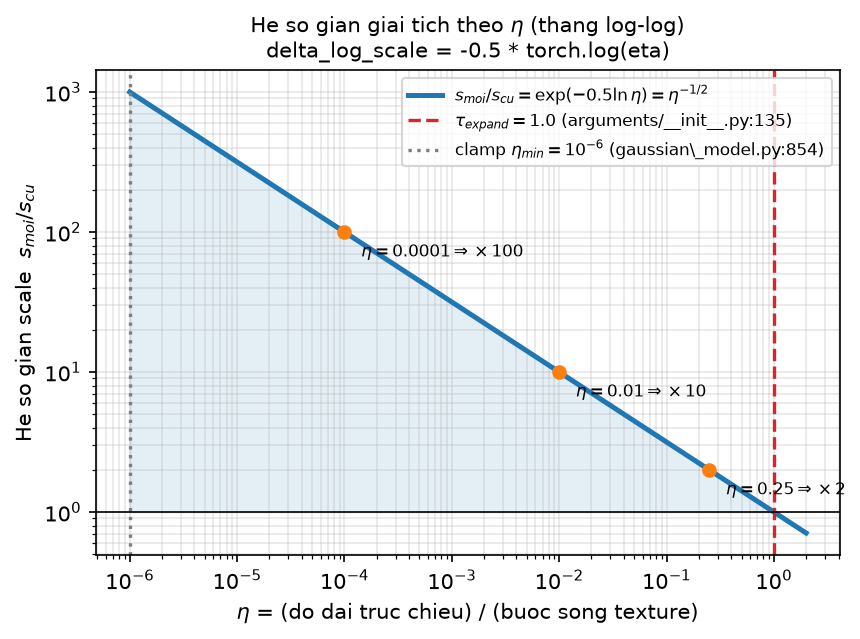
\includegraphics[width=0.99\linewidth]{sadgsx/06_scale_ratio_eta.png}\\
\captionof{figure}{\footnotesize Hệ số giãn $\eta^{-1/2}$ theo $\eta$ (log--log): chỉ vùng $\eta<\tau_{expand}$ bị tác động; clamp $10^{-6}$ giới hạn giãn ở $\approx 1000\times$.}
\end{column}
\end{columns}
\end{frame}

% ===== BOT 07: densify_and_prune_structgs — vòng densify+prune hợp nhất =====

\begin{frame}{SADGS: \texttt{densify\_and\_prune\_structgs} -- một vòng sinh + xoá hợp nhất}
\scriptsize
\begin{columns}[T]
\begin{column}{0.45\linewidth}
Mỗi $100$ iteration (từ iter $500$), \texttt{train.py:362} gọi một hàm duy nhất. Thứ tự thật trong code (\texttt{gaussian\_model.py:957--1053}):
\[
\textbf{CLONE} \rightarrow \textbf{SPLIT} \rightarrow \textbf{PRUNE} \rightarrow \text{trần } \alpha\!\le\!0.8
\]
Mặt nạ sinh ($\texttt{dense}=0.001$):
\[
\texttt{clone} = (S \vee Q)\wedge[s_{\max}\!\le\!\texttt{dense}\cdot\texttt{ext}]
\]
\[
\texttt{split} = (S \vee Q_{abs})\wedge[s_{\max}\!>\!\texttt{dense}\cdot\texttt{ext}]
\]
Mặt nạ xoá là \textbf{hợp OR của 4 tiêu chí}:
\[
\big[\alpha\!<\!0.1\big] \vee \big[r_{2D}\!>\!20\big] \vee \big[s_{\max}\!>\!0.1\,\texttt{ext}\big] \vee \big[\texttt{low\_ratio}\!>\!0.8\big]
\]
\begin{itemize}
    \item \texttt{min\_opacity} thật $=\mathbf{0.1}$ (\texttt{train.py:364}), gấp $20\times$ mức $0.005$ của 3DGS gốc.
    \item $r_{2D}$ và $s_{\max}$ chỉ xét sau iter $3000$ (trước đó \texttt{max\_screen\_size}$=$\texttt{None}).
    \item \texttt{low\_ratio} được pad $0$ cho Gaussian vừa sinh $\Rightarrow$ chúng miễn nhiễm tiêu chí multi-view ở chính vòng này.
    \item \texttt{pruning\_score=None} $\Rightarrow$ nhánh multinomial $50\%$ không chạy: xoá cứng toàn bộ ứng viên.
    \item \texttt{prune\_points} dùng \texttt{valid}$=\lnot$\texttt{mask} cắt đồng bộ 6 tham số, mọi bộ đếm $\eta$, và \texttt{exp\_avg}/\texttt{exp\_avg\_sq} của \textbf{cả} \texttt{optimizer} lẫn \texttt{shoptimizer}.
\end{itemize}
\end{column}
\begin{column}{0.53\linewidth}
\begin{center}
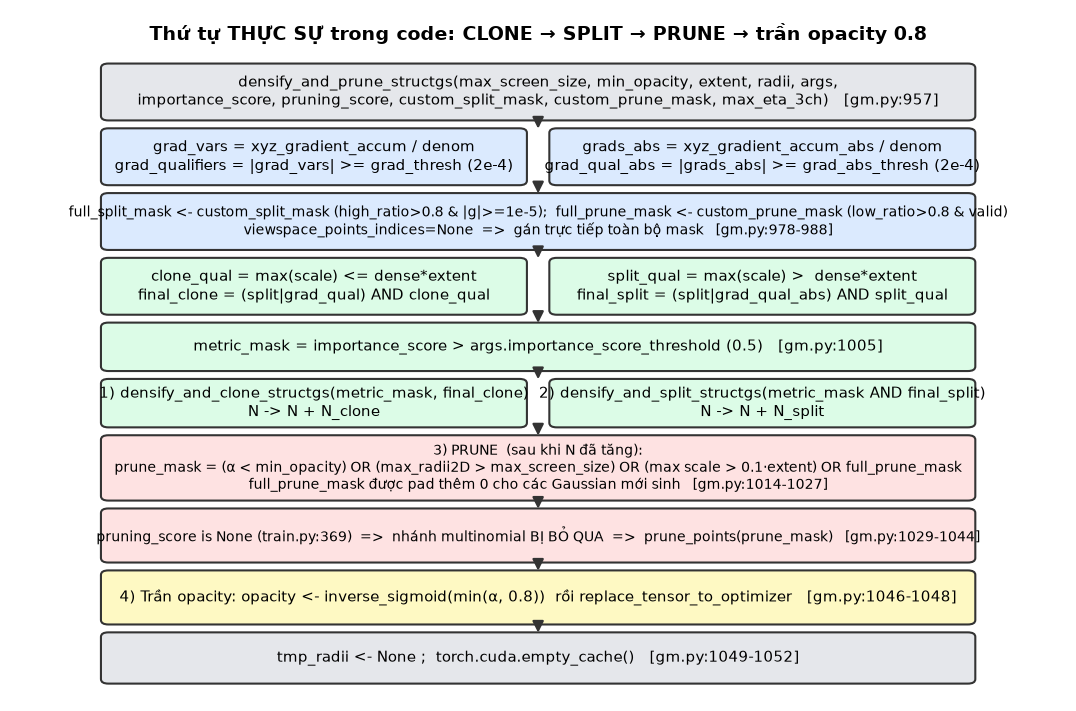
\includegraphics[width=0.99\linewidth]{sadgsx/07_so_do_khoi_luong.png}
\captionof{figure}{\scriptsize Luồng thật của \texttt{densify\_and\_prune\_structgs}: prune luôn chạy \textbf{sau} khi $N$ đã tăng, nên Gaussian con mới sinh cũng bị soi bởi ngưỡng opacity/bán kính/scale.}
\end{center}
\end{column}
\end{columns}
\end{frame}

% ===== BOT 08: final_prune_structgs — prune cuối theo pruning score & multi-view consistency =====

\begin{frame}{Tỉa cuối \texttt{final\_prune\_structgs}: công thức có, lời gọi đang tắt}
\scriptsize
\begin{columns}[T]
\begin{column}{0.50\textwidth}
Toàn bộ hàm (\texttt{scene/gaussian\_model.py:1059--1066}) là một phép OR tất định:
\[
\text{prune}_i=\big[\alpha_i<\tau_\alpha\big]\;\vee\;\big[s_i>\tau_s\big]
\]
với $\tau_\alpha=\texttt{min\_opacity}=0{,}1$ (lời gọi \texttt{train.py:419}) và $\tau_s=0{,}9$ \textbf{hard-code} ở \texttt{:1064}; $s_i$ là \texttt{pruning\_score} -- độ \emph{bất nhất} tái dựng qua nhiều view. Mặt nạ đi thẳng vào \texttt{prune\_points} (\texttt{:528}), cắt cả tham số lẫn mọi bộ đếm $\eta$.
\begin{itemize}
    \item Chạy tại \texttt{prune\_iterations} mặc định \texttt{[4000, 8000]} (\texttt{train.py:412, 529}).
    \item Khác prune trong vòng densify: ở đó có \texttt{remove\_budget = int(0.5*to\_remove)} + \texttt{multinomial} (\texttt{:1029--1042}); ở đây cắt dứt khoát, không phanh.
    \item \alert{Lời gọi bị comment} (\texttt{train.py:418--419}); nguồn điểm số \texttt{compute\_gaussian\_score\_structgs} \textbf{không tồn tại} trong repo; mặc định \texttt{pruning\_score=None} sẽ gây \texttt{TypeError} vì \texttt{:1064} không kiểm tra None.
    \item Cái thực chạy chỉ còn $[\alpha_i<0{,}1]$ (\texttt{train.py:416--417}) $\Rightarrow$ floater (opacity cao, chỉ đúng vài view) lọt lưới, mô hình cuối to hơn cần thiết.
\end{itemize}
\end{column}
\begin{column}{0.48\textwidth}
\centering
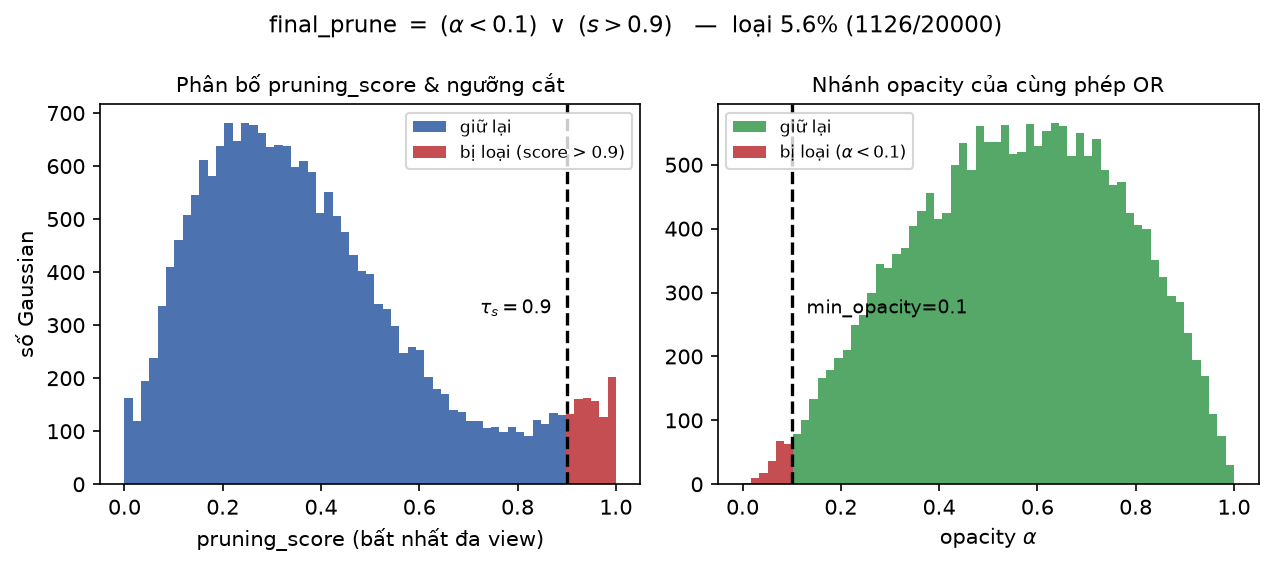
\includegraphics[width=\linewidth]{sadgsx/08_score_hist.png}
\captionof{figure}{\footnotesize Hai nhánh của phép OR: $\tau_s=0{,}9$ chỉ cắt đuôi bất nhất, $\tau_\alpha=0{,}1$ cắt opacity yếu (code ghi rõ \texttt{\# 0.005 is a good default}, \texttt{train.py:364}).}
\end{column}
\end{columns}
\end{frame}

% ===== BOT 09: Optimizer, learning-rate schedule & opacity reset trong SADGS =====

\begin{frame}{Optimizer, lịch learning rate \& reset opacity trong SADGS}
\scriptsize
\begin{columns}[T]
\begin{column}{0.52\textwidth}
\textbf{1. Lịch lr vị trí} (\texttt{get\_expon\_lr\_func}, \texttt{general\_utils.py:32--64}):
\[
\mathrm{lr}(k)=\exp\!\big[(1-t)\ln lr_{\text{init}} + t\ln lr_{\text{fin}}\big],\; t=\mathrm{clip}\!\big(\tfrac{k}{30000},0,1\big)
\]
với $lr_{\text{init}}=1.6\!\times\!10^{-4}\!\cdot s$, $lr_{\text{fin}}=1.6\!\times\!10^{-6}\!\cdot s$. \texttt{lr\_delay\_steps} không được truyền ($=0$) nên warm-up \textbf{không kích hoạt}.
\vspace{0.12cm}

\textbf{2. lr hằng số các nhóm khác} (\texttt{training\_setup:306--313}): \texttt{opacity} $0.05$, \texttt{scaling} $0.01$, \texttt{rotation} $0.002$, \texttt{f\_dc} $0.0025$, \texttt{f\_rest} $=0.005/20$ -- ba nhóm đầu \textbf{gấp đôi} 3DGS gốc.
\vspace{0.12cm}

\textbf{3. Optimizer} \texttt{hybrid} (mặc định): Adam+\texttt{amsgrad} cho hình học $\oplus$ \texttt{SparseGaussianAdam} cho SH bậc cao (chỉ cập nhật Gaussian có \texttt{radii>0}), $\varepsilon=10^{-8}$.
\vspace{0.12cm}

\textbf{4. Reset opacity} mỗi $3000$ iter (\texttt{train.py:402}):
\[
\alpha_{\text{new}}=\frac{\sigma(o)\,c\cdot 0.1}{c}=0.1\,\sigma(o)
\]
hệ số 3D filter $c$ \textbf{triệt tiêu} $\Rightarrow$ chỉ là phép \textbf{nhân} $0.1$; khác 3DGS gốc kẹp $\min(\alpha,0.01)$ -- SADGS \textbf{giữ nguyên thứ tự} độ đục rồi prune ở ngưỡng $0.1$.
\vspace{0.12cm}

\textbf{5. Bậc SH}: \texttt{oneupSHdegree} gọi \textbf{mỗi iteration} $\Rightarrow d_k=\min(k,3)$, bão hoà ngay tại $k=3$ (3DGS: mỗi 1000 iter).
\end{column}
\begin{column}{0.46\textwidth}
\centering
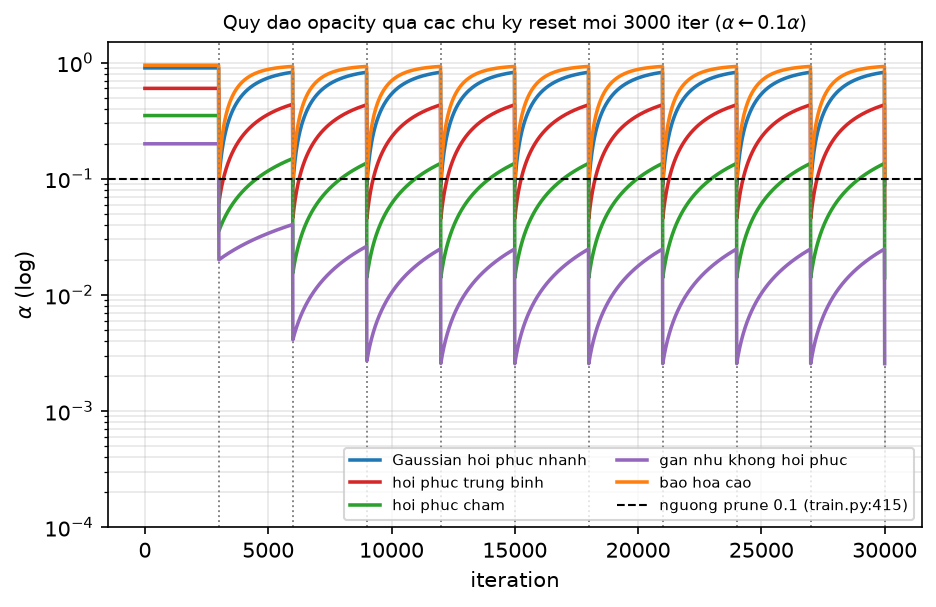
\includegraphics[width=\linewidth]{sadgsx/09_opacity_reset_traj.png}
\captionof{figure}{\scriptsize Quỹ đạo $\alpha$ (log) qua 10 chu kỳ reset $\alpha\!\leftarrow\!0.1\alpha$; đường đứt là ngưỡng prune $0.1$.}
\end{column}
\end{columns}
\end{frame}

% ===== BOT 10: Bộ lọc 3D chống alias (3D filter / Mip-splatting style) trong SADGS =====

\begin{frame}{Bộ lọc 3D chống alias: chặn dưới kích thước Gaussian theo Nyquist}
\scriptsize
\begin{columns}[T]
\begin{column}{0.52\textwidth}
\textbf{1. Ngưỡng lọc} (\texttt{gaussian\_model.py:254}) --- $z$ là \textbf{độ sâu} tới camera \textit{gần nhất} nhìn thấy Gaussian (\texttt{:245}), $f=\max_i f_x^{(i)}$ của camera phân giải cao nhất (\texttt{:247}):
\[
\texttt{filter\_3D} = \frac{z}{f}\sqrt{0.2}\;\;\approx\;0.447\times(\text{1 pixel quy về 3D})
\]
\textbf{2. Scale hiệu dụng} (\texttt{:156--161}) --- tích chập Gaussian$*$Gaussian, $\Sigma\!\to\!\Sigma+\sigma_f^2 I$:
\[
s_i^{\text{eff}}=\sqrt{s_i^2+\texttt{filter\_3D}^2}\;\xrightarrow{\;s_i\to 0\;}\;\sigma_f
\]
\textbf{3. Bù opacity} (\texttt{:190--201}) --- bảo toàn năng lượng $\alpha\sqrt{\det\Sigma}$:
\[
\texttt{coef}=\sqrt{\frac{\prod_i s_i^2}{\prod_i (s_i^2+\sigma_f^2)}},\quad
\alpha^{\text{eff}}=\alpha\cdot\texttt{coef}
\]
đẳng hướng: $\texttt{coef}=(1+r^2)^{-3/2}$, $r=\sigma_f/s$.
\end{column}
\begin{column}{0.48\textwidth}
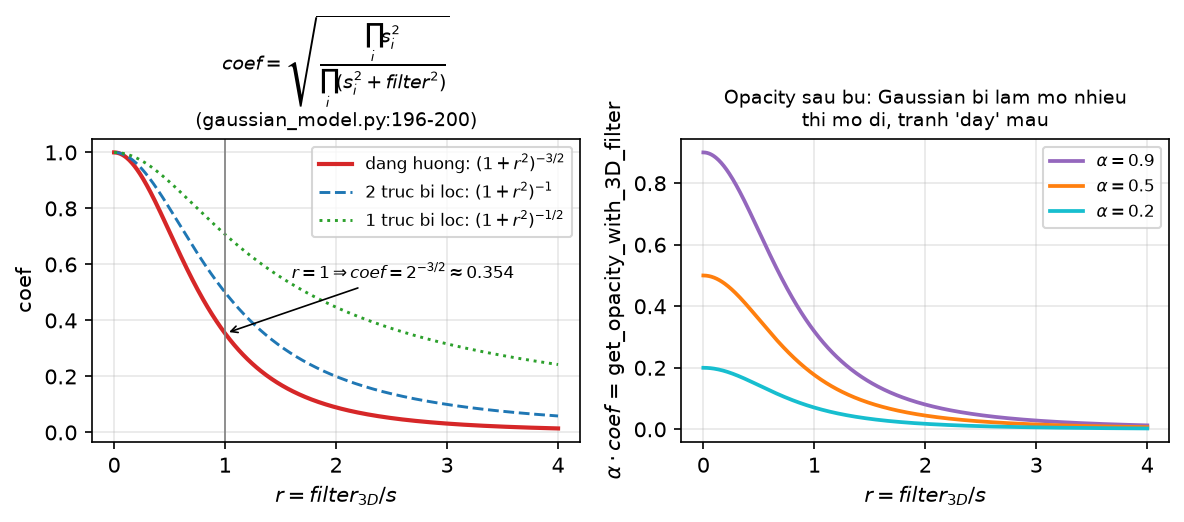
\includegraphics[width=\linewidth]{sadgsx/10_opacity_coef.png}
\captionof{figure}{\scriptsize Hệ số bù opacity theo $r=\texttt{filter\_3D}/s$: Gaussian nhỏ hơn pixel bị \textbf{mờ đi} thay vì nhấp nháy.}
\end{column}
\end{columns}
\vspace{0.1cm}
\begin{itemize}
    \item Dùng ở render: \texttt{opacity} (\texttt{gaussian\_renderer:63}), \texttt{scales} (\texttt{:74}). Bật bằng \texttt{--compute\_3d\_filter} (mặc định \texttt{False}, \texttt{arguments:132}); tắt $\Rightarrow$ \texttt{filter\_3D}$=0$ (\texttt{train.py:158}).
    \item Cập nhật: 1 lần trước vòng lặp (\texttt{train.py:155}), sau đó mỗi \textbf{100 iteration} nhưng \textbf{chỉ sau} \texttt{densify\_until\_iter}$=15000$ và dừng trước 100 bước cuối (\texttt{train.py:405--409}). Con sinh ra khi densify \textbf{kế thừa} \texttt{filter\_3D} của cha (\texttt{:728, :886, :907}); prune lọc theo mask (\texttt{:547--548}).
    \item \textbf{Với $\eta$}: SADGS chia $k_i=\lceil\sqrt{\eta_i}\rceil$ để làm $s$ nhỏ đi; bộ lọc 3D là \textbf{phanh} --- khi $s\lesssim\sigma_f$, $s^{\text{eff}}$ bão hoà còn \texttt{coef} sụp $\Rightarrow$ con quá nhỏ mất opacity và bị prune (\texttt{train.py:416}).
\end{itemize}
\end{frame}

% ===== BOT 11: Hàm mất mát của SADGS — L1, SSIM, tone-curve, frequency loss =====

\begin{frame}{Hàm mất mát của SADGS: $L_1$ + SSIM + $L_2$ (và hai loss chưa dùng)}
\scriptsize
\begin{columns}[T]
\begin{column}{0.47\linewidth}
\textbf{Loss thực sự được tối ưu} --- \texttt{train.py:259}:
\[
\mathcal{L} = (1-\lambda_{\text{dssim}})L_1 + \lambda_{\text{dssim}}(1-\mathrm{SSIM}) + \lambda_{L_2} L_2
\]
\[
= \;0.8\,L_1 \;+\; 0.2\,(1-\mathrm{SSIM}) \;+\; \mathbf{2.0}\,L_2
\]
$\lambda_{\text{dssim}}=0.2$, $\lambda_{L_2}=2.0$ (\texttt{arguments/\_\_init\_\_.py:86,117}). SSIM dùng kernel CUDA \texttt{fused\_ssim} (\texttt{train.py:18,258}), không dùng \texttt{ssim()} thuần torch ở \texttt{loss\_utils.py:46} (cửa sổ Gaussian $11\times11$, $\sigma=1.5$, $C_1=0.01^2$, $C_2=0.03^2$).
\vspace{3pt}

\alert{Hai loss được định nghĩa nhưng KHÔNG vào $\mathcal{L}$:}
\begin{itemize}
    \item \texttt{tone\_curve\_loss} (\texttt{:28}): $\;\dfrac{1}{N}\sum\Bigl(\dfrac{p-g}{\mathrm{sg}(p)+\varepsilon}\Bigr)^{2}$, $\varepsilon=10^{-6}$ --- chia sai số cho độ sáng dự đoán (stop-gradient) $\Rightarrow$ học trên \emph{sai số tương đối}, khuếch đại gradient vùng tối.
    \item \texttt{frequency\_loss} (\texttt{:80}): $\;\dfrac{1}{N}\sum \mathrm{ReLU}\bigl(\sigma_{\text{lin}} - \lambda_{\text{lim}}\bigr)$ với $\sigma_{\text{lin}}=\sqrt{\sqrt{\det\Sigma_{2D}}}$ và $\lambda_{\text{lim}} = 1/\sqrt{S_{xx}+S_{yy}}$ lấy mẫu từ \texttt{st\_map} tại \texttt{means2D} --- phạt Gaussian \textbf{to hơn bước sóng} texture.
\end{itemize}
Cả hai có trọng số $=0$ và \textbf{không được tham chiếu} ở bất kỳ đâu (\texttt{lambda\_tone}, \texttt{lambda\_freq} --- \texttt{args:118-119}).
\end{column}
\begin{column}{0.51\linewidth}
\centering
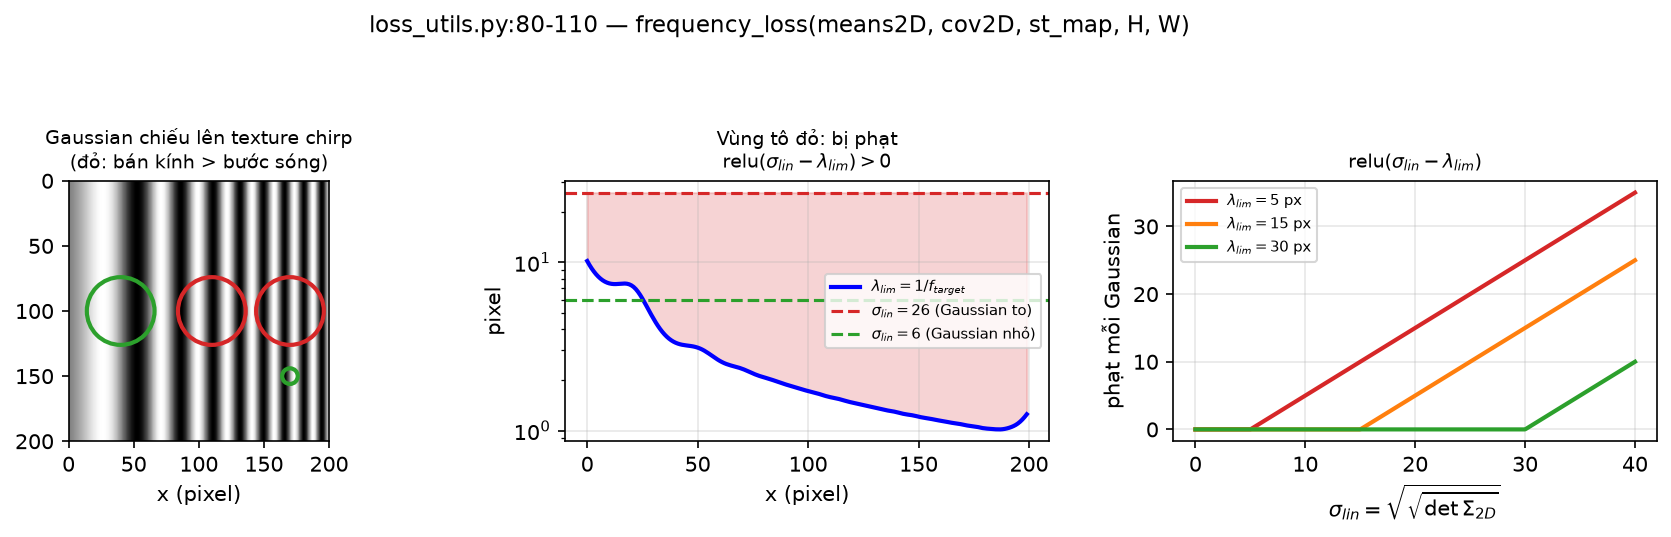
\includegraphics[width=\linewidth]{sadgsx/11_frequency_loss.png}
\captionof{figure}{\scriptsize \texttt{frequency\_loss} (\texttt{loss\_utils.py:80-110}): bước sóng cho phép $\lambda_{\text{lim}}$ co lại ở vùng texture rậm; Gaussian có $\sigma_{\text{lin}}$ vượt ngưỡng bị phạt tuyến tính một phía.}
\end{column}
\end{columns}
\vspace{2pt}
\begin{itemize}
    \item[$\Rightarrow$] Loss của SADGS $=$ loss 3DGS gốc \textbf{$+$ một số hạng $L_2$ trọng số lớn}. Cơ chế "structure-aware" nằm ở \textbf{densification} (thống kê $\eta$ không gradient, \texttt{freq\_utils.py:181}) chứ không nằm trong hàm mất mát.
\end{itemize}
\end{frame}

% ===== BOT 12: Chọn mẫu camera (FPS sampling) & lấy mẫu Gaussian dị hướng 2D =====

\begin{frame}{Lấy mẫu camera bằng FPS \& lấy mẫu Gaussian dị hướng 2D}
\scriptsize
\begin{columns}[T]
\column{0.47\linewidth}
\textbf{\texttt{sampling\_cameras}} (\texttt{utils/freq\_utils.py:12--87}), mặc định \texttt{mode="fps", num\_cams=60}. Vị trí camera $c_i=-R^{\top}t$ (dòng 47), rồi tham lam:
\[ d_i \!\leftarrow\! \min\big(d_i, \lVert c_i-c_{i_{k-1}}\rVert_2\big),\quad i_k=\arg\max_i d_i \]
\alert{Metric chỉ dùng VỊ TRÍ, không dùng hướng nhìn.} Chi phí $O(N\cdot\texttt{num\_cams})$ $\Rightarrow$ phải lấy tập con để thống kê tần số $\eta$ đủ rẻ.

\vspace{0.3em}
\textbf{\texttt{sample\_anisotropic\_gaussians\_2d}} (\texttt{utils/gaussian\_sampling.py:11}): vị trí $\sim p\propto S_{xx}\!+\!S_{yy}$; hình dạng từ $\lambda_{1,2}=\frac{\mathrm{tr}S}{2}\pm\sqrt{(\frac{\mathrm{tr}S}{2})^2-\det S}$, trục dài dọc $v_2$ (hướng cạnh).

\vspace{0.3em}
\alert{Sự thật cần nêu:} hàm này \emph{không} được gọi ở đâu; khởi tạo point cloud vẫn là \texttt{create\_from\_pcd} từ COLMAP (\texttt{scene/\_\_init\_\_.py:83}). Và ở \texttt{train.py:224,240} FPS được gọi với \texttt{num\_cams=len(stack)} nên chỉ thay thế \texttt{random.shuffle}.

\column{0.51\linewidth}
\centering
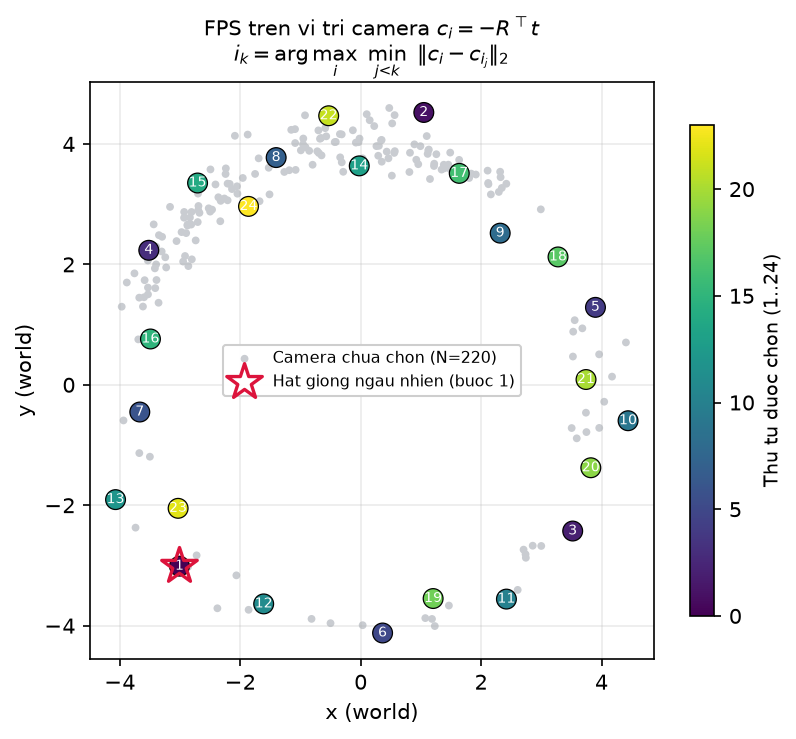
\includegraphics[width=\linewidth]{sadgsx/12_fps_selection.png}
\captionof{figure}{\footnotesize FPS trên tập vị trí camera: màu/số là thứ tự chọn --- mẫu trải đều dù mật độ camera gốc rất lệch.}
\end{columns}
\end{frame}

% ===== BOT 13: Toàn bộ siêu tham số của SADGS & lịch trình huấn luyện thực tế =====

\begin{frame}{Siêu tham số \& lịch trình huấn luyện của SADGS}
\scriptsize
\begin{columns}[T]
\begin{column}{0.44\textwidth}
\textbf{Các cờ MỚI quan trọng nhất} (\texttt{arguments/\_\_init\_\_.py})
\begin{tabular}{ll}
\toprule
\textbf{Cờ} & \textbf{Mặc định} \\
\midrule
\texttt{mult} & \texttt{0.7} \\
\texttt{eta\_compute\_mode} & \texttt{"wavelength"} \\
\texttt{split\_ratio\_threshold} & \texttt{0.8} \\
\texttt{prune\_ratio\_threshold} & \texttt{0.8} \\
\texttt{dense} & \texttt{0.001} \\
\texttt{freq\_grad\_threshold} & \texttt{2e-5} \\
\texttt{freq\_opacity\_threshold} & \texttt{0.05} \\
\texttt{opacity\_reset\_decay} & \texttt{0.1} \\
\texttt{highfeature\_lr} & \texttt{0.005} ($/20$) \\
\texttt{lambda\_l2} & \texttt{2.0} \\
\texttt{optimizer\_type} & \texttt{"hybrid"} \\
\texttt{warmup\_densification} & \texttt{False} \\
\bottomrule
\end{tabular}
\vspace{0.12cm}\\
$\tau_{high}=1.0$, $\tau_{low}=0.1$ \textbf{hard-code} trong \texttt{freq\_utils.py:395--396}.
\vspace{0.1cm}\\
\textbf{Lịch trình:} SH lên bậc mỗi iter; cập nhật $\eta$ mỗi 10 iter (đến 15k); densify mỗi 100 iter (500--15k) rồi xoá bộ đếm $\eta$; reset opacity mỗi 3k ($\alpha\!\leftarrow\!0.1\alpha$); prune thô tại 4k/8k; 15k--30k chỉ tinh chỉnh.
\vspace{0.08cm}\\
\textbf{Bị comment-out:} \texttt{expand\_undersized\_gs} ($\Rightarrow$ \texttt{tau\_expand} vô hiệu), prune warmup, \texttt{final\_prune\_structgs}.
\end{column}
\begin{column}{0.56\textwidth}
\centering
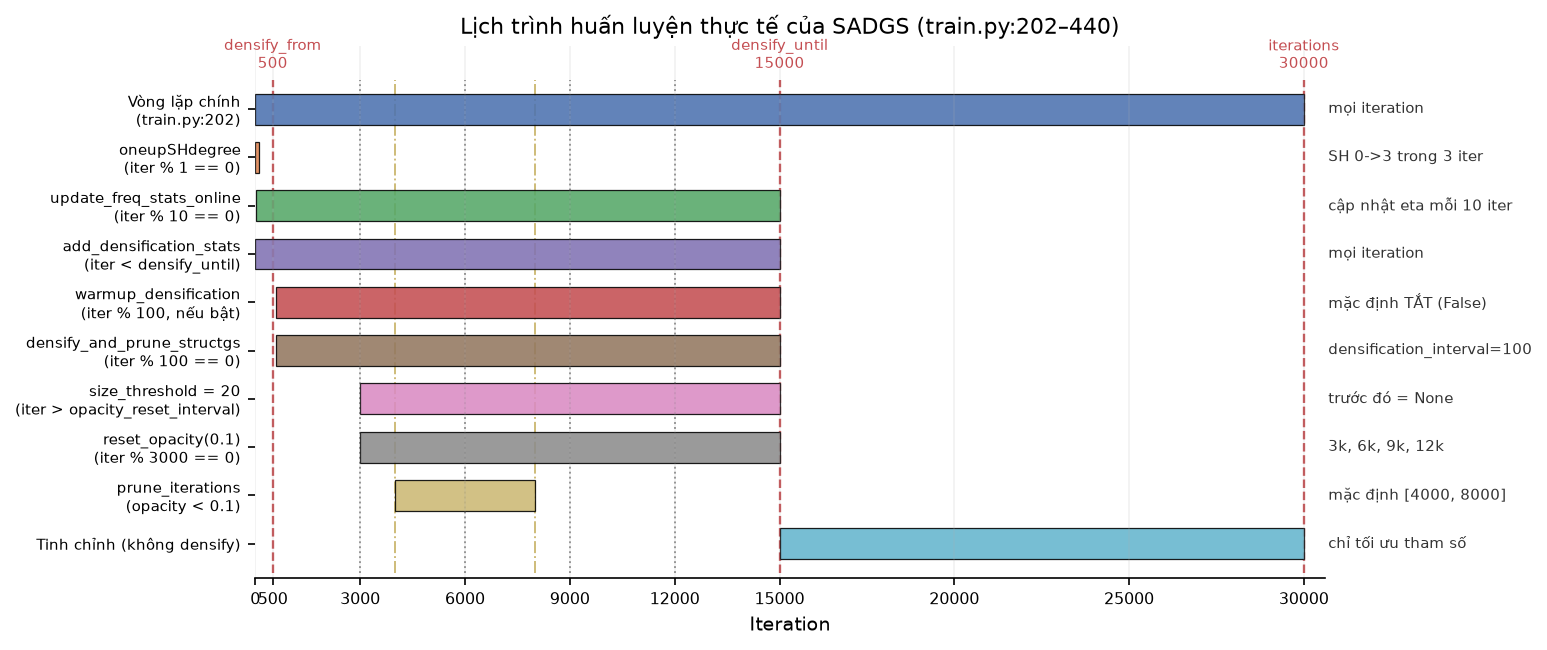
\includegraphics[width=\linewidth]{sadgsx/13_lich_trinh.png}
\captionof{figure}{\scriptsize Lịch trình huấn luyện thật dựng từ \texttt{train.py:202--440}.}
\end{column}
\end{columns}
\end{frame}

% ===== BOT 14: Rasterizer riêng của SADGS — diff-gaussian-rasterization\_structgs =====

\begin{frame}{Rasterizer riêng của SADGS: \texttt{mult}, \texttt{cov2D} và $T^{\max}$}
\scriptsize
\begin{columns}[T]
\begin{column}{0.50\textwidth}
SADGS fork rasterizer CUDA của 3DGS thành \texttt{diff-gaussian-rasterization\_structgs}, gọi qua \texttt{render\_structgs(\dots, mult, \dots)} (\texttt{gaussian\_renderer/\_\_init\_\_.py:18}).
\vspace{0.1cm}
\textbf{1. Nền tảng không đổi} --- tile $16\times16$ (\texttt{config.h:16--17}), sort theo $\big[\text{tile}|\text{depth}\big]$, alpha blending:
\[
\alpha_i=\sigma_{o,i}e^{-\frac12 d_i^\top\Sigma_{2D,i}^{-1}d_i},\;\;
T_i=\!\!\prod_{j<i}\!(1-\alpha_j),\;\;
C=\sum_i c_i\alpha_iT_i
\]
bỏ qua $\alpha<1/255$, dừng sớm khi $T<10^{-4}$.
\vspace{0.1cm}
\textbf{2. \texttt{mult} --- compact box} thay AABB $3\sigma$: chỉ gán tile cho vùng
\[
d^\top\Sigma_{2D}^{-1}d\le t,\qquad t=\texttt{mult}\cdot 2\ln(255\,\sigma_o)
\]
(\texttt{auxiliary.h:332--333}). Mặc định \texttt{opt.mult}$=0.7$ (\texttt{arguments/\_\_init\_\_.py:114}) $\Rightarrow$ ít cặp (tile,\,Gaussian) $\Rightarrow$ sort ngắn, render nhanh; phần bị cắt có $\alpha$ dưới cả ngưỡng $1/255$ nên chất lượng gần như không đổi.
\end{column}
\begin{column}{0.49\textwidth}
\centering
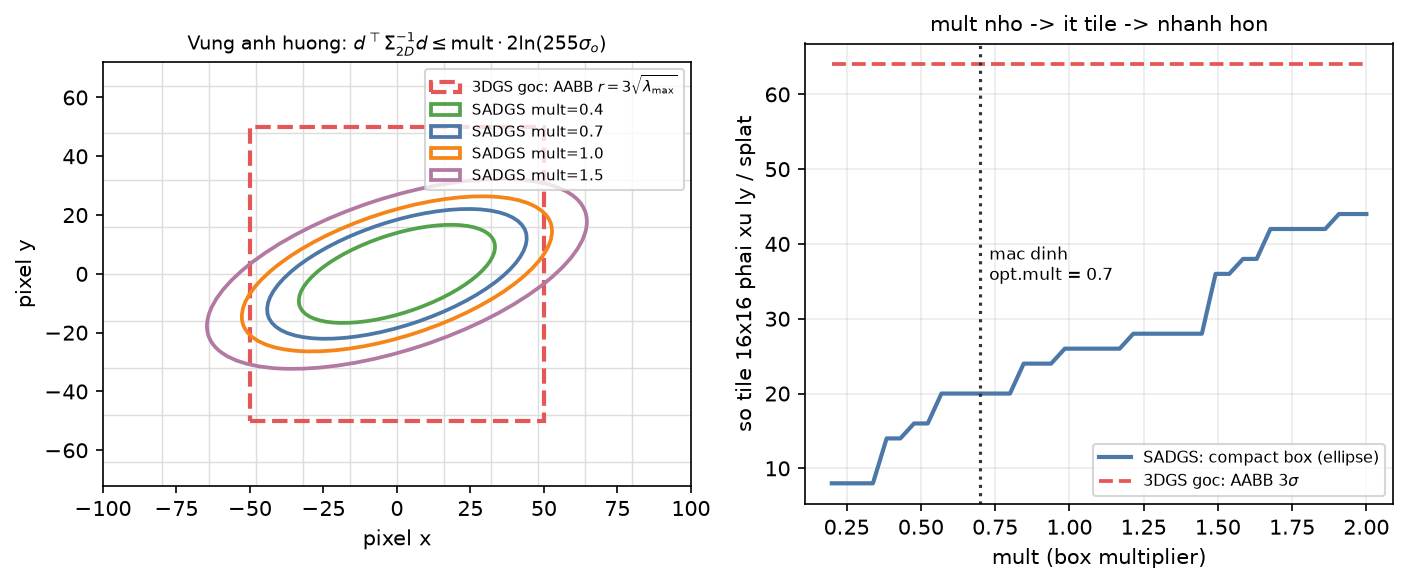
\includegraphics[width=0.99\linewidth]{sadgsx/14_mult_vs_3sigma.png}
\captionof{figure}{\footnotesize Vùng ảnh hưởng theo \texttt{mult} so với AABB $3\sigma$ và số tile $16\times16$ phải xử lý mỗi splat.}
\raggedright
\vspace{0.1cm}
\textbf{3. Đầu ra mới: \texttt{cov2D} $(N,7)$} (\texttt{rasterize\_points.cu:92})
\begin{itemize}\itemsep0pt
    \item cột 0--2: $\Sigma_{2D}$; cột 3--4: tâm pixel; cột 5: depth (\texttt{forward.cu:241--246})
    \item cột 6: $T^{\max}$ ghi bằng \texttt{atomicMax} trên bit-pattern float (\texttt{forward.cu:470})
\end{itemize}
Python lọc $\big(T^{\max}\!>\!\tau_T\big)\wedge\big(\sigma_o\!>\!\tau_o{=}0.05\big)$ rồi lấy mẫu Cholesky từ $\Sigma_{2D}$ để tính $\eta$ (\texttt{utils/freq\_utils.py:181--260}). Kèm theo: \texttt{accum\_metric\_counts}, \texttt{depth/opacity/normal\_map} khi \texttt{compute\_extra}.
\end{column}
\end{columns}
\end{frame}

% ===== BOT 15: Tổng hợp đầu-cuối SADGS (bản 45 phút — 1 frame) =====
\begin{frame}{Tổng hợp đầu-cuối: pipeline SADGS, chi phí, và phần chưa bật}
\scriptsize
\begin{columns}[T]
\begin{column}{0.52\textwidth}
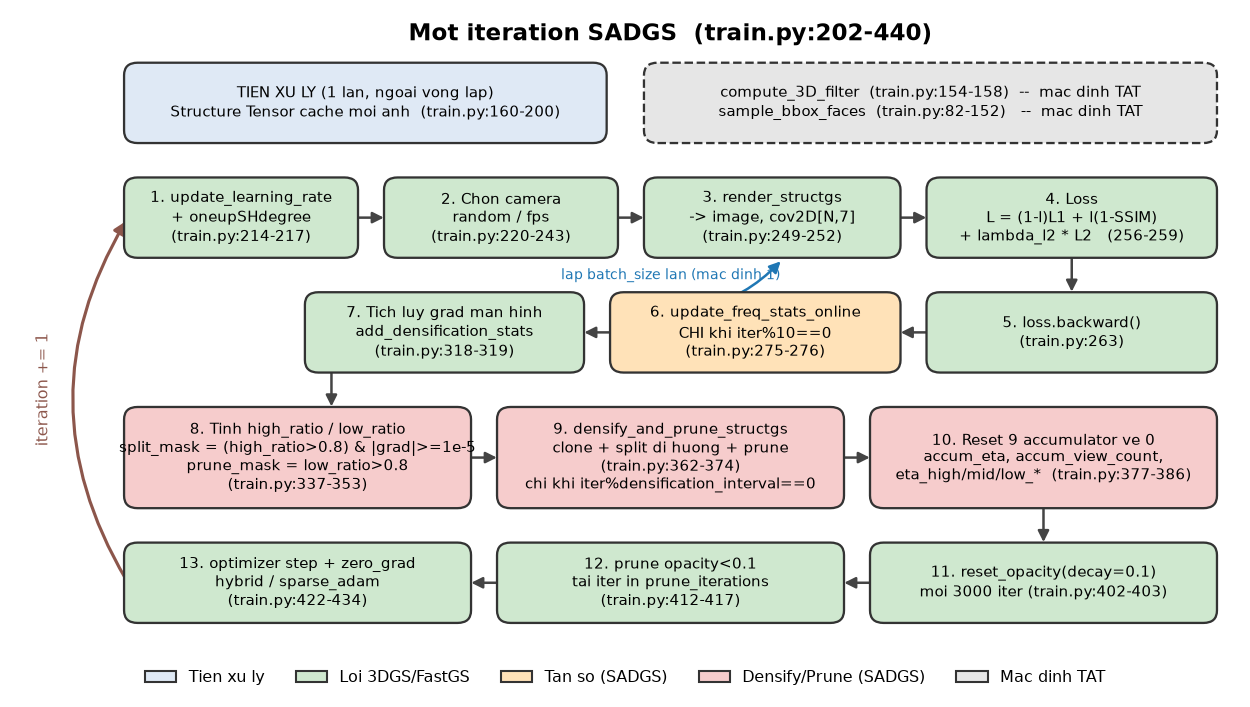
\includegraphics[width=0.99\linewidth]{sadgsx/15_pipeline_blocks.png}\\[0.5mm]
\captionof{figure}{\tiny 13 bước của một iteration SADGS (\texttt{train.py:202--440}); khối xám nét đứt = mặc định TẮT.}
\end{column}
\begin{column}{0.46\textwidth}
\textbf{Chi phí mỗi vòng:}
\begin{equation*}
t_{\text{iter}} = a N + b P + c + \tfrac{a_\eta N}{10} + \tfrac{a_D N}{100}
\end{equation*}
Freq stats chỉ chạy khi \texttt{iter\%10==0} (\texttt{train.py:275}); densify chỉ khi \texttt{iter\%100==0}. Vì $t$ tuyến tính theo $N$, \textbf{prune đa view} (\texttt{low\_ratio}$>0.8$) là đòn bẩy mạnh nhất.
\vspace{1mm}

\textbf{Khác biệt cốt lõi so với 3DGS gốc} (\texttt{densify\_and\_clone}/\texttt{densify\_and\_split}, \texttt{scene/gaussian\_model.py})\textbf{:} tín hiệu densify là AND của gradient và \texttt{high\_ratio}$>0.8$; split \emph{dị hướng} $k_{\text{axis}}{=}\lceil\sqrt{\eta_{\text{axis}}}\rceil$; prune thêm tiêu chí đa view. Nền rasterization (compact box \texttt{mult}$=0.7$, Sparse Adam) giữ nguyên.
\vspace{1mm}

\alert{\textbf{Đã cài nhưng KHÔNG chạy:}} \texttt{expand\_undersized\_gs} (\texttt{train.py:356--359}), \texttt{final\_prune\_structgs} (\texttt{418--419}), prune warmup (\texttt{393--400}), \texttt{training\_report} (\texttt{306}), \texttt{scene.save} (\texttt{442}) --- đều bị comment; cộng 10 cờ mặc định \texttt{False} và 6 tham số dead code.
\vspace{1mm}

\textbf{Rủi ro đo đạc:} \texttt{render.py:40--44} đo FPS không \texttt{cuda.synchronize()}; \texttt{metrics.py:74} dùng SSIM khác hàm với lúc train; \texttt{full\_eval.py:90,95,121} truyền \texttt{--budget/--mode/--sh\_lower} \emph{chưa được khai báo} trong \texttt{arguments}.
\end{column}
\end{columns}
\end{frame}


\section{Tổng kết}
% ============================================================
% PHẦN 45 phút — Slide 39-42 (Quan sát RAM, Tổng kết pipeline,
% Tổng kết SADGS & giới hạn, Cảm ơn / Q&A) — rút gọn từ part7.tex
% (Số slide +1 so với bản trước do part45_09.tex được bổ sung 1 frame mới
% về cơ chế lõi structure-aware densification.)
% ============================================================

% --- Slide 39 (gốc: Slide 62 — Quan sát 2) ---
\begin{frame}{Quan sát 2: Nút thắt là RAM hệ thống, không phải VRAM}
\begin{itemize}
    \item Đo trên Google Colab T4 trong quá trình huấn luyện:
\end{itemize}
\footnotesize
\begin{table}[]
\centering
\begin{tabular}{lccc}
\toprule
Tài nguyên & Đỉnh sử dụng & Khả dụng & \% sử dụng \\
\midrule
VRAM (GPU) & 1.16 GB & 14.56 GB & \textbf{8\%} \\
RAM hệ thống & 9.59 GB & 12.7 GB & \textbf{91\%} (giới hạn mềm 10.5 GB) \\
\bottomrule
\end{tabular}
\end{table}
\normalsize
\begin{itemize}
    \item RAM hệ thống áp sát giới hạn mềm, trong khi VRAM còn dư rất nhiều.
    \item Khuyến nghị cũ "giảm độ phân giải để tiết kiệm VRAM" \textbf{không cần thiết} ở ngân sách này.
\end{itemize}
\end{frame}

% --- Slide 40 (gốc: Slide 64 — Tổng kết pipeline) ---
\begin{frame}{Tổng kết pipeline render 3D Gaussian Splatting}
\centering
\footnotesize
\begin{tikzpicture}[
    node distance=8mm and 6mm,
    box/.style={draw, rounded corners, align=center, minimum height=0.9cm, minimum width=2.6cm, fill=blue!8}
]
\node[box] (gauss) {3D Gaussian\\$(\mu,\Sigma,\alpha,SH)$};
\node[box, right=of gauss] (proj) {Chiếu phối cảnh\\(EWA)};
\node[box, right=of proj] (raster) {Rasterizer khả vi\\theo tile};

\node[box, below=of raster] (blend) {Alpha\\blending};
\node[box, left=of blend] (loss) {Loss\\($L_1$+D-SSIM)};
\node[box, left=of loss] (back) {Backward\\(gradient)};

\node[box, below=of back, fill=orange!12] (adc) {Adaptive\\Density Control};

\draw[-Latex] (gauss) -- (proj);
\draw[-Latex] (proj) -- (raster);
\draw[-Latex] (raster) -- (blend);
\draw[-Latex] (blend) -- (loss);
\draw[-Latex] (loss) -- (back);
\draw[-Latex] (back) -- (adc);
\draw[-Latex] (adc) -- (gauss);
\end{tikzpicture}
\vspace{2mm}

\normalsize
Một chu trình khép kín: render $\rightarrow$ tính loss $\rightarrow$ lan truyền ngược $\rightarrow$ điều chỉnh mật độ Gaussian $\rightarrow$ lặp lại.
\end{frame}

% --- Slide 41 (gốc: Slide 65 — Tổng kết cải tiến SADGS \& giới hạn) ---
\begin{frame}{Tổng kết cải tiến SADGS \& giới hạn còn lại}
\footnotesize
\textbf{Đóng góp cốt lõi + các đòn bẩy hiệu năng:}
\begin{itemize}
    \item \textbf{Structure-aware densification} (đóng góp chính, Slide 33): so khớp kích thước Gaussian với bước sóng texture qua tỉ số $\eta$; split \textbf{dị hướng theo trục} ($k_{\text{axis}}=\lceil\sqrt{\eta_{\text{axis}}}\rceil$) thay vì luôn tách 2 như 3DGS gốc $\Rightarrow$ mật độ Gaussian bám sát độ chi tiết ảnh thay vì đồng nhất.
    \item \textbf{Multi-view score} + \textbf{Compact box} $\Rightarrow$ giảm Gaussian dư thừa mà không giảm chất lượng đáng kể.
    \item \textbf{Sparse Adam} $\Rightarrow$ giảm chi phí tính toán mỗi iteration.
\end{itemize}
\vspace{2mm}
\textbf{Giới hạn / hướng phát triển:}
\begin{enumerate}
    \item \texttt{expand\_undersized\_gs} (giãn giải tích Gaussian dưới cỡ) và \texttt{final\_prune\_structgs} (prune cuối theo multi-view consistency) \textbf{đã cài đặt đúng} trong \texttt{gaussian\_model.py} nhưng lời gọi \textbf{đang bị comment out} trong \texttt{train.py} $\Rightarrow$ không chạy trong lịch huấn luyện mặc định, kể cả khi tăng ngân sách iteration.
    \item Dữ liệu Gaussian đầu ra chưa được nén (248 B/Gaussian, thô).
    \item Chưa có ablation study cô lập riêng từng đòn bẩy.
    \item 4 nhánh mở rộng của SADGS gốc — dynamic scenes, sparse view, surface reconstruction, SLAM — chưa tích hợp vào fork này.
\end{enumerate}
\end{frame}

% --- Slide 42 (gốc: Slide 67 — Cảm ơn / Q&A, frame cuối cùng) ---
\begin{frame}[c]{}
\centering
{\Huge \textbf{Cảm ơn đã theo dõi!}}

\vspace{6mm}
{\LARGE Hỏi đáp (Q\&A)}

\vspace{10mm}
{\small Digital Twin GS --- SADGS \\ \texttt{github.com/KietAnhCS/SADGS}}
\end{frame}
   % Slide 39-42 RAM vs VRAM, Tổng kết pipeline, Tổng kết cải tiến, Cảm ơn/Q&A

\end{document}
